\documentclass[11 pt, a4paper]{report}
%\documentclass[11pt,twoside, journal]{IEEEtran}
\usepackage{lipsum}
\usepackage{printlen}
\usepackage{etex}
\usepackage[dvips]{graphicx}
 \usepackage[table, dvipsnames]{xcolor}
 \renewcommand{\arraystretch}{1.2}
\usepackage[]{hhline}
\usepackage{comment}
\excludecomment{toexclude}
\usepackage[top=3.7cm, bottom=3cm]{geometry}
\DeclareGraphicsRule{.pdf}{pdf}{.pdf}{}
\DeclareGraphicsRule{*}{eps}{*}{}
\usepackage{lipsum}
%\usepackage[T5]{fontenc}
\usepackage[utf8]{inputenc}
\usepackage[vietnam,english]{babel}
\usepackage{lmodern}
\usepackage{amssymb} 
\usepackage{textcomp}
\usepackage{blindtext}
\usepackage[reqno]{amsmath}
\usepackage{psfrag}
\usepackage{multirow}
\usepackage{tabularx}
\setlength{\extrarowheight}{3pt}
\usepackage{array}
\usepackage{dcolumn}
%apparently will allow footnotes inside tables!
\usepackage{pdflscape}
%\numberwithin{equation}
 \usepackage[usenames,dvipsnames]{pstricks}
\usepackage{pst-node}
\usepackage{pstricks-add}
%no idea why this is here, but it turned all the \mathit\deltas into black squares!
%\usepackage{mathpazo,tgpagella}
\usepackage{booktabs,pst-plot}
\usepackage{epsfig}
\usepackage{rotating}
\usepackage{xkeyval}
\usepackage{pst-3dplot}
\usepackage{paralist} %for inline enumeration use begin{inparaenum}[(a)]
\usepackage{upgreek}
\usepackage{url}
\usepackage{stfloats} % for spanning floats, apparently a bit aggresive!
% for footnotes at bottom, not glued to text
\usepackage[bottom]{footmisc}
\usepackage{titlesec}
\makeatletter
\renewcommand{\@makechapterhead}[1]{%
\vspace*{-10 pt}%
{\setlength{\parindent}{0pt} \raggedright \normalfont
\LARGE\thechapter.\ #1
\par\nobreak\vspace{20 pt}}}

\renewcommand{\@makeschapterhead}[1]{%
\vspace*{0 pt}%
{\setlength{\parindent}{0pt} \raggedright \normalfont
\LARGE#1
\par\nobreak\vspace{20 pt}}}

\renewcommand\section{\@startsection {section}{1}{\z@}%
                                   {-3.5ex \@plus -1ex \@minus -.2ex}%
                                   {2.3ex \@plus.2ex}%
                                   {\Large\itshape}}
                                   
\renewcommand\subsection{\@startsection{subsection}{2}{\z@}%
                                     {-3.25ex\@plus -1ex \@minus -.2ex}%
                                     {1.5ex \@plus .2ex}%
    								{\large\scshape}}
\makeatother

  
%\usepackage{draftwatermark}
%\SetWatermarkText{\parbox{40cm}{%
% \centering DRAFT \\
% {Not for circulation}} }
%\SetWatermarkScale{0.4}

%\usepackage[printwatermark]{xwatermark}

%\newwatermark[allpages,color=gray!50, angle=45,scale=3,xpos=0,ypos=0]{DRAFT}
\usepackage[labelfont={bf, it}]{caption}
  
\newcommand{\R}{R}
\usepackage{hyperref}
\hypersetup{
    colorlinks,
    citecolor=black,
    linkcolor=black,
	urlcolor=black,
	breaklinks=true
}
\usepackage[hyphenbreaks]{breakurl}


\usepackage{csquotes}
\usepackage[
natbib=true,
style=authoryear-ibid,
maxbibnames=3,
maxcitenames=2,
uniquelist=false,
%firstinits=true,
backend=bibtex,
url=true,
bibencoding=ascii,
]{biblatex}
\setlength\bibitemsep{1.5\itemsep}


\bibliography{foresight}

\setlength{\parskip}{1em}
\usepackage{fancyhdr} 

\pagestyle{fancy} 
\fancyhead{} 
\fancyfoot{} 
\renewcommand{\headrulewidth}{1pt}
\fancypagestyle{plain}
{
 \fancyhf{}
\fancyhead[C]{\small \emph{Foresight Trends}\\\tiny}
\fancyfoot[C]{\thepage}
}
\pagestyle{plain}
\renewcommand{\labelitemii}{$\rightarrow$}

\begin{document}
\title{\Large {\emph{Foresight Trends}}\\ \vspace{2cm}
\LARGE{Future of an Ageing Population}\\ \vspace{4cm}}



\author{George Leeson, Nana Nanitashvili \& Maja Zalo\v znik
%\textit{Authors}
\\
\textsc{\small The Oxford Institute of Population Ageing}\\ \vspace*{1cm} } 
\date{\small July 2016}

%
\maketitle

\setcounter{secnumdepth}{1}
\setcounter{tocdepth}{5}
\tableofcontents

\chapter{Population Ageing – age-structural change} %1

\subsection{Population Structure}
\begin{figure}[htbp!]
\psfrag{A}[c][c]{2015}
\psfrag{B}[c][c]{1950}
\psfrag{C}[c][c]{1925}

\psfrag{95}[c][c]{\small{95}}
\psfrag{90}[c][c]{\small{90}}
\psfrag{85}[c][c]{\small{85}}
\psfrag{80}[c][c]{\small{80}}
\psfrag{75}[c][c]{\small{75}}
\psfrag{70}[c][c]{\small{70}}
\psfrag{65}[c][c]{\small{65}}
\psfrag{60}[c][c]{\small{60}}
\psfrag{55}[c][c]{\small{55}}
\psfrag{50}[c][c]{\small{50}}
\psfrag{45}[c][c]{\small{45}}
\psfrag{40}[c][c]{\small{40}}
\psfrag{35}[c][c]{\small{35}}
\psfrag{30}[c][c]{\small{30}}
\psfrag{25}[c][c]{\small{25}}
\psfrag{20}[c][c]{\small{20}}
\psfrag{15}[c][c]{\small{15}}
\psfrag{19}[c][c]{\small{10}}
\psfrag{51}[c][r]{\small{5}}
\psfrag{91}[c][r]{\small{0}}
\psfrag{x}{\small{\emph{Males}}}
\psfrag{y}{\small{\emph{Females}}}

\psfrag{l}[ct][cb]{\small{\emph{Percentage of the population}}}
\psfrag{a}[r][c]{\small{\emph{Age}}}
\psfrag{2}{\small{2 \%}}
\psfrag{4}{\small{4 \%}}
\psfrag{6}{\small{6 \%}}
\psfrag{8}{\small{8 \%}}
\psfrag{0}{\small{0 \%}}
\psfrag{10}{\small{10 \%}}

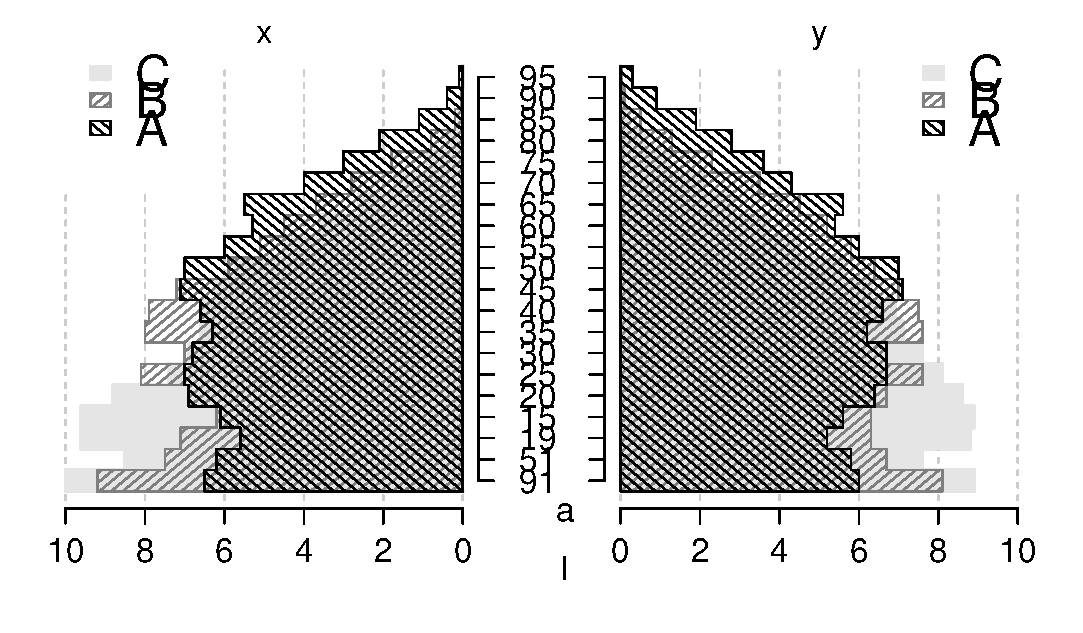
\includegraphics[width=\textwidth]{../figures/Fig1.1.eps}
\caption{The population distribution of the United Kingdom by age group for 1925, 1950 and 2015. Source: \citet{ONS2013b} and  \citet{HMD2015}}\label{Fig:01}
\end{figure}

In the United Kingdom, the 20th century saw a dramatic transformation of the population pyramid as the changes in fertility, early life and then later life mortality passed into and through the age profile of the population. This is of course a continual process and so the population structure of the future will reflect the increasing longevity predicted for males and females as well as – at most – modest increases in fertility. The age structures 1925, 1950 and 2015 are shown in Figure \ref{Fig:01} (and the data in Table \ref{Tab:11}. It is clear for both males and females that the typical age pyramid of 1925 (albeit with the base beginning to narrow) had changed dramatically to a distribution where the proportions in younger age groups have declined while those in mid- and later-life age groups have increased. For example, in 1925, the proportions of the population in the United Kingdom aged under 15 years were 28 per cent for males and 25 per cent for females. By 2015, these had declined to 18 and 17 per cent respectively. On the other hand, the proportions aged over 65 years have in the same period increased from 6 and 7 per cent to 16 and 19 per cent.  It is not possible to understand these trends without reference to fertility and mortality change.

\begin{table}[hbtp!]

\caption{The population distribution of the United Kingdom by age group for 1925, 1950 and 2015 (see Figure \ref{Fig:01}). Source: \citet{ONS2013b} and  \citet{HMD2015}.}\label{Tab:11}
\centering
\vspace{2ex}

\begin{tabularx}\textwidth{p{3cm} *6{>{\centering\arraybackslash}X}@{}}
\hline 
 & \multicolumn{3}{c}{\emph{Males}} & \multicolumn{3}{c}{\emph{Females}}\\ 
 \cline{2-7}
 & 1925 & 1950 & 2015 & 1925 & 1950 & 2015 \\ 
  \hline
   0 -- 4 & 10.00 & 9.20 & 6.50 & 8.90 & 8.10 & 6.00 \\ 
   5  -- 9& 8.50 & 7.50 & 6.20 & 7.60 & 6.70 & 5.80 \\ 
   10 -- 14 & 9.60 & 7.10 & 5.60 & 8.80 & 6.30 & 5.20 \\ 
   15 -- 19 & 9.60 & 6.20 & 6.10 & 8.90 & 6.30 & 5.60 \\ 
   20 -- 24 & 8.80 & 6.90 & 6.90 & 8.60 & 6.70 & 6.40 \\ 
   25 -- 29& 7.40 & 8.10 & 7.00 & 8.10 & 7.60 & 6.70 \\ 
   30 -- 34& 6.90 & 7.00 & 6.80 & 7.60 & 6.70 & 6.70 \\ 
   35 -- 39& 6.60 & 8.00 & 6.30 & 7.10 & 7.60 & 6.20 \\ 
   40 -- 44& 6.60 & 7.90 & 6.60 & 6.90 & 7.50 & 6.60 \\ 
   45 -- 49& 6.20 & 7.20 & 7.10 & 6.30 & 7.00 & 7.10 \\ 
   50 -- 54& 5.70 & 5.90 & 7.00 & 5.60 & 6.40 & 7.00 \\ 
   55 -- 59& 4.50 & 5.10 & 6.00 & 4.50 & 5.80 & 6.00 \\ 
   60 -- 64& 3.60 & 4.50 & 5.30 & 3.70 & 5.20 & 5.40 \\ 
   65 -- 69& 2.60 & 3.70 & 5.50 & 2.80 & 4.50 & 5.60 \\ 
   70 -- 74& 1.70 & 2.80 & 4.00 & 2.10 & 3.50 & 4.30 \\ 
   75 -- 79& 0.90 & 1.80 & 3.00 & 1.20 & 2.30 & 3.60 \\ 
   80 -- 84& 0.40 & 0.80 & 2.10 & 0.60 & 1.30 & 2.80 \\ 
   85 -- 89& 0.10 & 0.20 & 1.10 & 0.20 & 0.50 & 1.90 \\ 
   90 -- 94& 0.02 & 0.04 & 0.40 & 0.05 & 0.10 & 0.90 \\ 
   over 95 & 0.00 & 0.00 & 0.09 & 0.01 & 0.02 & 0.30 \\ 
   \hline
\end{tabularx}
\end{table}

\clearpage
%%%%%%%%%%%%%%%%%%%%%%%%%%%%
\subsection{Fertility Rates}

\begin{figure}[hbtp!]
\psfrag{2012}[r][r]{\small{2012}}
\psfrag{2010}[r][r]{\small{2010}}
\psfrag{2000}[r][r]{\small{2000}}
\psfrag{1990}[r][r]{\small{1990}}
\psfrag{1980}[r][r]{\small{1980}}
\psfrag{1970}[r][r]{\small{1970}}
\psfrag{1965}[r][r]{\small{1965}}
\psfrag{2005}[r][r]{\small{2005}}
\psfrag{1995}[r][r]{\small{1995}}
\psfrag{1985}[r][r]{\small{1985}}
\psfrag{1975}[r][r]{\small{1975}}
\psfrag{1960}[r][r]{\small{1960}}
\psfrag{tfr}[c][c]{\normalsize{\emph{Total Fertility Rate}}}
\psfrag{0.0}{\small{0.0}}
\psfrag{0.5}{\small{0.5}}
\psfrag{1.0}{\small{1.0}}
\psfrag{1.5}{\small{1.5}}
\psfrag{2.0}{\small{2.0}}
\psfrag{2.5}{\small{2.5}}
\psfrag{3.0}{\small{3.0}}
\psfrag{3.5}{\small{3.5}}
\psfrag{y}{\small{\emph{Year}}}

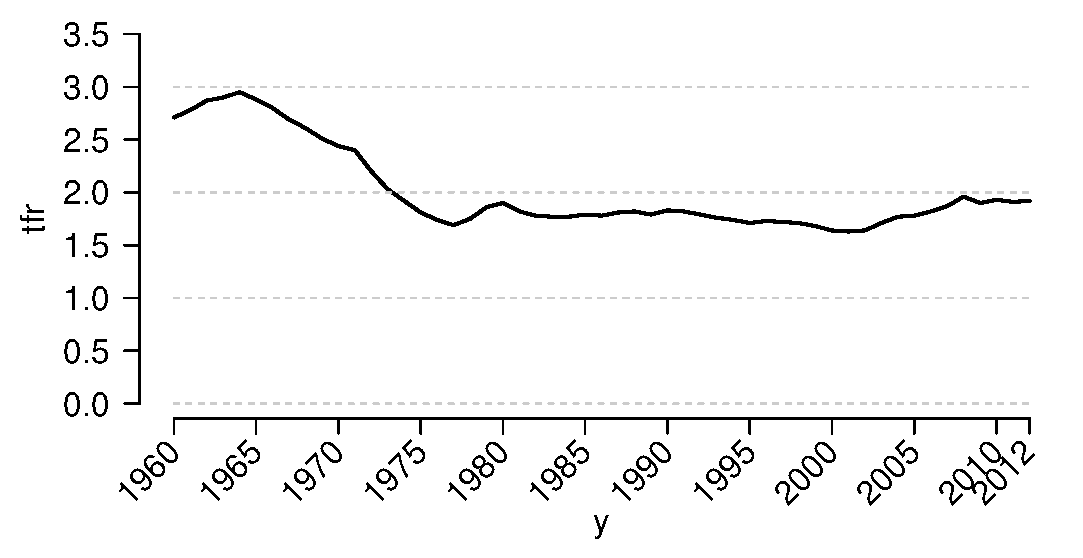
\includegraphics[width=\textwidth]{../figures/Fig1.2.eps}
\caption{Total fertility in the United Kingdom, 1960-2012 Source: \citet{ONS2014}}
\label{Fig:03}
\end{figure}

Fertility in the United Kingdom fell towards replacement level in the continued fertility decline of the demographic transition (for example, \cite{Kirk1996}) and then to below replacement in the second demographic transition \citep{vdKaa1987}, leaving the United Kingdom still in a low fertility cycle after almost 40 years of below replacement fertility. Since 1973, total fertility has been below replacement level, and although some argue that recent evidence would suggest increasing total fertility, arguing that fertility in the United Kingdom is now at a level (approximately 1.9) not experienced since 1974, it has to be noted that the previous increase from 1977 until 1980 was followed by a more prolonged decline until 2001. 

 
\begin{table}[ht]

\caption{Total fertility in the United Kingdom, 1960-2012 (see Figure \ref{Fig:03}). Source: \citet{ONS2014}}\label{Tab:12}
\centering
\vspace{2ex}
\centering
\begin{tabular}{lr<{\hspace{-2pt}}r<{\hspace{-2pt}}r<{\hspace{-2pt}}r<{\hspace{-2pt}}r<{\hspace{-2pt}}r<{\hspace{-2pt}}r<{\hspace{-2pt}}r<{\hspace{-2pt}}r<{\hspace{-2pt}}r<{\hspace{-2pt}}r<{\hspace{-2pt}}r<{\hspace{-2pt}}}
  \hline
 \small 
Year &1960 & 1965 & 1970 & 1975& 1980 & 1985 & 1990 & 1995& 2000 & 2005& 
2010& 2012 \\ 
\hline
TFR &  2.71 & 2.88 & 2.44 & 1.81 & 1.90 & 1.79 & 1.83 & 1.71 & 1.64 & 1.78 & 1.93 & 1.92 \\ 
   \hline
   
\end{tabular}
\end{table}

\clearpage


\begin{figure}[hbtp!]
\psfrag{l}[c][c][1][45]{\scriptsize{2013}}
\psfrag{k}[c][c][1][45]{\scriptsize{2010}}
\psfrag{i}[c][c][1][45]{\scriptsize{2000}}
\psfrag{g}[c][c][1][45]{\scriptsize{1990}}
\psfrag{e}[c][c][1][45]{\scriptsize{1980}}
\psfrag{c}[c][c][1][45]{\scriptsize{1970}}
\psfrag{b}[c][c][1][45]{\scriptsize{1965}}
\psfrag{j}[c][c][1][45]{\scriptsize{2005}}
\psfrag{h}[c][c][1][45]{\scriptsize{1995}}
\psfrag{f}[c][c][1][45]{\scriptsize{1985}}
\psfrag{d}[c][c][1][45]{\scriptsize{1975}}
\psfrag{a}[c][c][1][45]{\scriptsize{1960}}
\psfrag{0.0}[c][c]{\small{0.0}}
\psfrag{0.5}[c][c]{\small{0.5}}
\psfrag{1.0}[c][c]{\small{1.0}}
\psfrag{1.5}[c][c]{\small{1.5}}
\psfrag{2.0}[c][c]{\small{2.0}}
\psfrag{2.5}[c][c]{\small{2.5}}
\psfrag{3.0}[c][c]{\small{3.0}}
\psfrag{3.5}[c][c]{\small{3.5}}
\psfrag{y}[c][c]{\small{\emph{Total Fertility Rate}}}
\psfrag{A}[l][l]{\emph{Dual-Earner} or \emph{Social Democratic}}
\psfrag{B}[l][l]{\emph{Liberal} or \emph{Market Oriented}}
\psfrag{C}[l][l]{\emph{General Family Support} or \emph{Conservative}}
\psfrag{D}[l][l]{\emph{Transition Post-Socialist}}
\psfrag{E}[l][l]{\emph{Familialistic or Mediterranean}}
\psfrag{x}[c][c]{\emph{Year}}

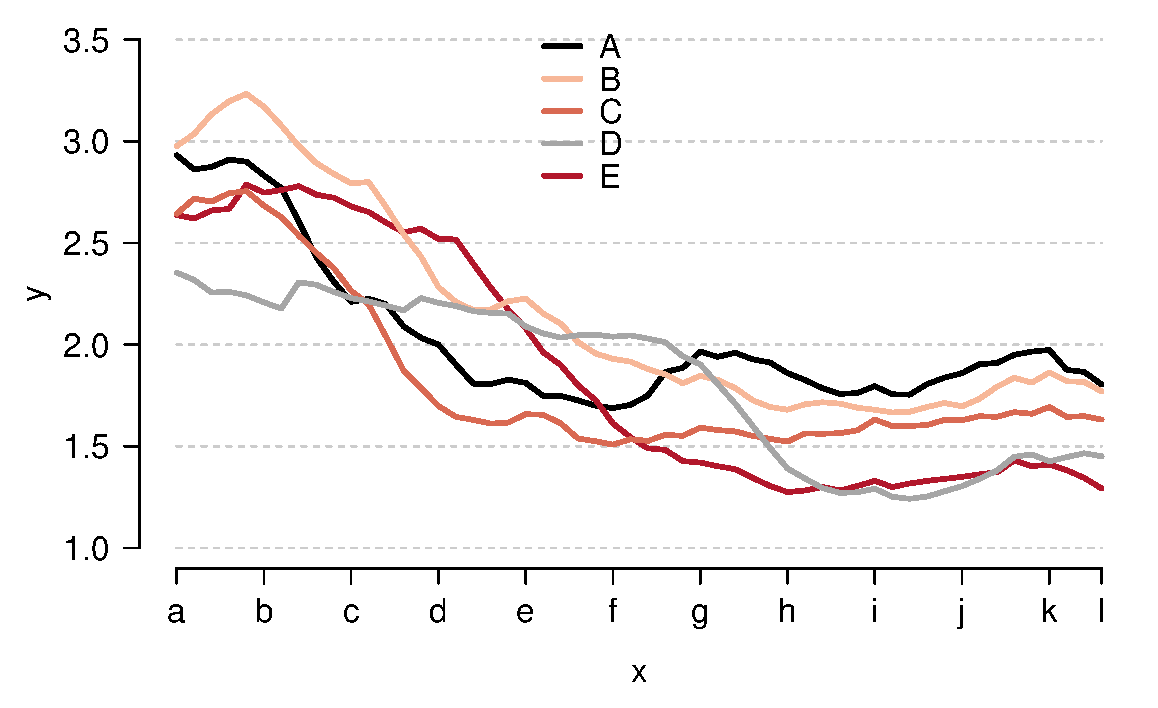
\includegraphics[width=\textwidth]{../figures/Fig1.3.eps}
\caption{Total fertility in EU countries (1960-2013), grouped by welfare regime/policy configuration type (see text for explanation). Source: \cite{INED2016} for 1960-2010 and \cite{EUST2016} for 2011-2013.}
\label{Fig:03.1}
\end{figure}

\noindent The different policy configuration types plotted in Figure \ref{Fig:03.1} are defined as follows \citep{Olah2014}):\label{Txt:defs}
\begin{itemize}   
\item \emph{Dual-Earner} policy configuration type or \emph{Social Democratic }welfare regime with extensive policy provision facilitating work-life balance for both women and men: Denmark, Finland, Iceland,Norway and Sweden;
\item \emph{Liberal} or \emph{Market-Oriented} regime with limited and usually means-tested state support to families and the dominance of market-based solutions regarding welfare provision: United Kingdom, Ireland and Switzerland;
\item \emph{General Family Support} policy configuration type or \emph{Conservative} welfare regime in which men's primacy at the labour market has not really been questioned while the range of state support to families and to women to combine paid work and family responsibilities varies greatly across countries:  Austria, Belgium, France, Germany (FRG only until 1990), Luxembourg and the Netherlands;
\item \emph{Familialistic} or \emph{Mediterranean} welfare regime with nearly none or extremely limited policy provision to families and pronounced gender role differentiation:  Greece, Italy, Portugal and Spain;
\item    \emph{Transition Post-Socialist} cluster which is also rather heterogeneous in terms of state support to families and to women to combine labour market participation and family life: Bulgaria, Czech Republic, Estonia, GDR (until 1989); Hungary, Latvia, Lithuania, Poland, Romania, Slovakia and Slovenia.
\end{itemize}


\begin{table}[hbtp!]
\caption{Total fertility in EU countries (1960-2013), grouped by welfare regime/policy configuration type (see text for explanation) (see Figure \ref{Fig:03.1}). Source: \cite{INED2016} for 1960-2010 and \cite{EUST2016} for 2011-2013.}\label{Tab:EUfert}
\vspace{1ex}

\centering
\def\tabularxcolumn#1{m{#1}}

\begin{tabularx}\textwidth{p{1cm} *6{>{\centering\arraybackslash \small}X}@{}}
\hline 
&& \emph{Dual-Earners:} & \emph{Familialistic:} &\emph{General Family Support:} &\emph{Liberal}: & \emph{Transition Post-Socialist:}\\
\cline{3-7}

 &United Kingdom 
 & Denmark, Finland, Iceland, Norway, Sweden&  
  Greece,   Italy,   Portugal, Spain    &
  Austria, Belgium, France, Germany (FRG only until 1990), Luxembourg, Netherlands &  United Kingdom, Ireland,  Switzerland & 
 Bulgaria, Czech Republic, Estonia, GDR (until 1989) Hungary, Latvia, Lithuania, Poland, Romania, Slovakia, Slovenia \\ 

  \hline
1960 & 2.71 & 2.93 & 2.64 & 2.64 & 2.98 & 2.35 \\ 
  1965 & 2.88 & 2.83 & 2.75 & 2.68 & 3.17 & 2.21 \\ 
  1970 & 2.44 & 2.21 & 2.68 & 2.27 & 2.79 & 2.23 \\ 
  1975 & 1.81 & 2.00 & 2.52 & 1.70 & 2.28 & 2.21 \\ 
  1980 & 1.90 & 1.81 & 2.08 & 1.66 & 2.23 & 2.09 \\ 
  1985 & 1.79 & 1.69 & 1.61 & 1.51 & 1.93 & 2.04 \\ 
  1990 & 1.83 & 1.97 & 1.42 & 1.59 & 1.85 & 1.90 \\ 
  1995 & 1.71 & 1.86 & 1.27 & 1.52 & 1.68 & 1.39 \\ 
  2000 & 1.64 & 1.80 & 1.33 & 1.63 & 1.68 & 1.29 \\ 
  2005 & 1.78 & 1.86 & 1.35 & 1.63 & 1.70 & 1.30 \\ 
  2010 & 1.93 & 1.97 & 1.41 & 1.69 & 1.86 & 1.43 \\ 
  2013 & 1.92 & 1.80 & 1.29 & 1.63 & 1.77 & 1.45 \\ 
   \hline
\end{tabularx}
\end{table}


\clearpage
\subsection{Mortality Rates}
\begin{figure}[hbtp!]
\psfrag{2012}[r][r]{\small{2012}}
\psfrag{2010}[r][r]{\small{2010}}
\psfrag{2000}[r][r]{\small{2000}}
\psfrag{1990}[r][r]{\small{1990}}
\psfrag{1980}[r][r]{\small{1980}}
\psfrag{1970}[r][r]{\small{1970}}
\psfrag{1965}[r][r]{\small{1965}}
\psfrag{2005}[r][r]{\small{2005}}
\psfrag{1995}[r][r]{\small{1995}}
\psfrag{1985}[r][r]{\small{1985}}
\psfrag{1975}[r][r]{\small{1975}}
\psfrag{1960}[r][r]{\small{1960}}
\psfrag{1953}[r][r]{\small{1953}}
\psfrag{1955}[r][r]{\small{1955}}
\psfrag{1960}[r][r]{\small{1960}}

\psfrag{CDR}{\normalsize{\emph{Crude death rate}}}
\psfrag{IMR}{\normalsize{\emph{Infant mortality rate}}}
\psfrag{x}[c][c]{\normalsize{\emph{Year}}}
\psfrag{y}[c][c]{\normalsize{\emph{Mortality rate}}}

\psfrag{0}{\small{0}}
\psfrag{10}{\small{10}}
\psfrag{20}{\small{20}}
\psfrag{30}{\small{30}}
\psfrag{15}{\small{15}}
\psfrag{25}{\small{25}}
\psfrag{5}{\small{5}}
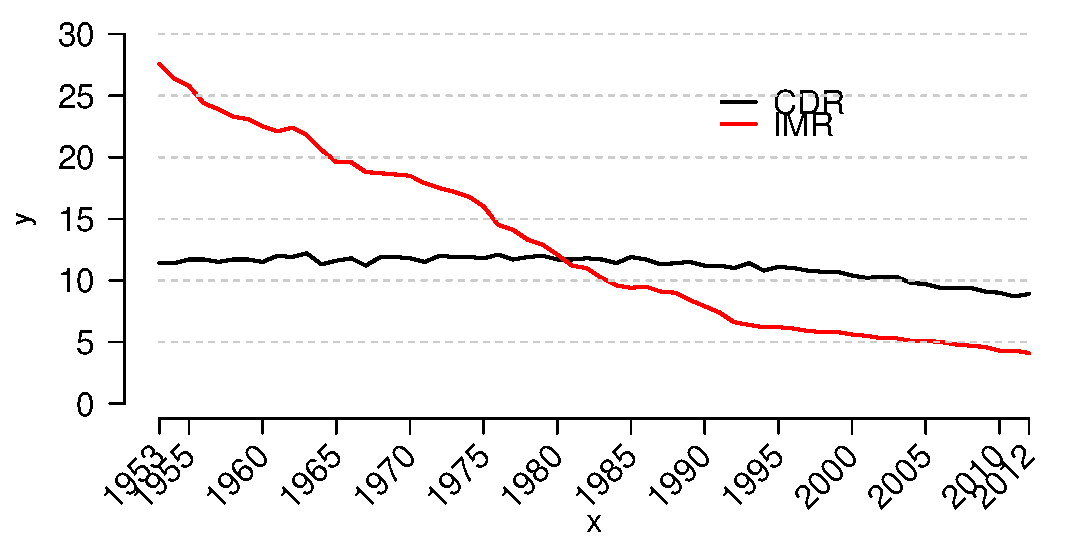
\includegraphics[width=\textwidth]{../figures/Fig1.4.eps}
\caption{Crude death rate (per 1000 population) and infant mortality rate (deaths under 1 year per 1000 live births) in the United Kingdom, 1953-2012. Source: ONS 2014a.}
\label{Fig:04}
\end{figure}


By 2012, the total number of deaths in the UK population (known as the Crude Death Rate (CDR)) was just over 569,000 corresponding to a CDR of 8.9 per 1000 population – still one of the lowest recorded for the United Kingdom \citep{ONS2014}. The CDR in the United Kingdom has declined modestly in the period 1953 to 1993 when it hovered above 11 after which it declined more strongly to 8.9 in 2013. On the other hand, the IMR has declined more dramatically over the 60 year period from just over 27 to just over 4.  By contrast, at the turn of the 20th century, IMR in the United Kingdom had been as high as 150 deaths under 1 year per 1000 live births \citep{ONS2014}, which corresponded to the infant mortality rate in India in the late 1950s (United Nations 2013). Indeed, declines in mortality among the extreme aged have been striking with the age-specific mortality rate for females in their early 80s, for example, in the United Kingdom declining from about 120 per 1000 population in the 1950s to 75 by the 1990s. Improvements have also occurred in that second half of the 20th century for males with rates for males in their early 80s falling from around 160 to 120. This has of course impacted on life expectancies in later life, as illustrated in section 2.

\begin{table}[hbtp!]

\caption{Crude death rate (per 1000 population) and infant mortality rate (deaths under 1 year per 1000 live births) in the United Kingdom, 1953-2012 (see Figure \ref{Fig:04}). Source: ONS 2014a. }\label{Tab:CDR}
\centering
\vspace{1ex}

\begin{tabular}{>{\small\hspace{-6pt}}l<{\hspace{-6pt}}>{\small}r<{\hspace{-6pt}}>{\small}r<{\hspace{-6pt}}>{\small}r<{\hspace{-6pt}}>{\small}r<{\hspace{-6pt}}>{\small}r<{\hspace{-6pt}}>{\small}r<{\hspace{-6pt}}>{\small}r<{\hspace{-6pt}}>{\small}r<{\hspace{-6pt}}>{\small}r<{\hspace{-6pt}}>{\small}r<{\hspace{-6pt}}>{\small}r<{\hspace{-6pt}}>{\small}r<{\hspace{-6pt}}>{\small}r<{\hspace{-6pt}}>{\small}r<{\hspace{-6pt}}}
  \hline
\emph{Year} & 1953 & 1955 & 1960 & 1965 & 1970 & 1975 & 1980 & 1985 & 1990 & 1995 & 2000 & 2005 & 2010 & 2012 \\ 
  \hline

\emph{CDR} &  11.40 & 11.70 & 11.50 & 11.60 & 11.80 & 11.80 & 11.70 & 11.90 & 11.20 & 11.10 & 10.40 & 9.70 & 9.00 & 8.90 \\ 
\emph{IMR} &  27.60 & 25.80 & 22.50 & 19.60 & 18.50 & 16.00 & 12.10 & 9.40 & 7.90 & 6.20 & 5.60 & 5.10 & 4.30 & 4.10 \\ 
   \hline
\end{tabular}
\end{table}

\clearpage




\subsection{Projected Population Structure}
\begin{figure}[hbtp!]

\psfrag{B}[c][c]{2015}
\psfrag{A}[c][c]{2040}

\psfrag{C}[c][c]{\scriptsize{ \textcolor{white}{0}0 -- 14}}
\psfrag{D}[c][c]{\scriptsize{ 15 -- 29}}
\psfrag{E}[c][c]{\scriptsize{ 30 -- 44}}
\psfrag{F}[c][c]{\scriptsize{ 45 -- 59}}
\psfrag{G}[c][c]{\scriptsize{ \textcolor{white}{03}60 -- 74}}
\psfrag{H}[c][c]{\scriptsize{ \textcolor{white}{0}75 \& over}}

\psfrag{5}{\small{5 \%}}
\psfrag{15}{\small{15 \%}}
\psfrag{20}{\small{20 \%}}
\psfrag{25}{\small{25 \%}}
\psfrag{0}{\small{0 \%}}
\psfrag{10}{\small{10 \%}}
\psfrag{XX}{\small{\emph{Males}}}
\psfrag{YY}{\small{\emph{Females}}}
\psfrag{a}[c][l]{\small{\emph{Age group}}}
\psfrag{y}[c][c]{\small{\emph{Percentage of the population}}}

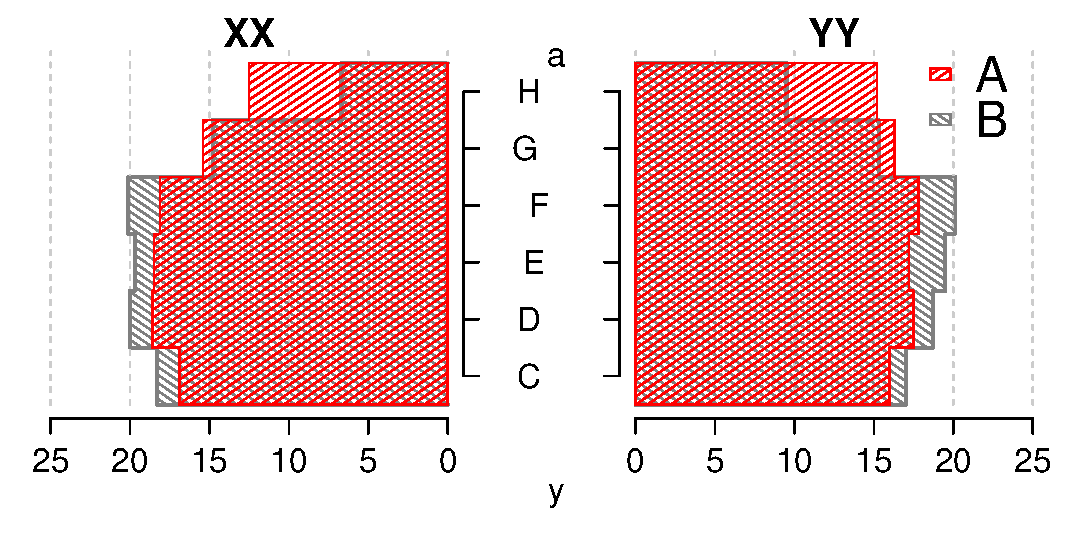
\includegraphics[width=\textwidth]{../figures/Fig1.5.eps}
\caption{Current and projected population distribution (principle variant) of the United Kingdom by age group, 2015 and 2040. Source: \cite{ONS2013b} and  \cite{HMD2015} }\label{Fig:05.5}
\end{figure}

It is clear for both males and females that the age pyramid for the United Kingdom continues to change dramatically moving forward to 2050 with the proportions in younger age groups continuing to decline and those in later-life age groups in particular increasing. In 2015, the proportions of the population aged 15-64 years were 65 per cent (males) and 64 per cent (females). By 2050, these have declined to 60 and 57 per cent respectively. On the other hand, the proportions aged over 65 years will in the same period increase from 16 and 19 per cent to 23 and 27 per cent.


\begin{table}[hbtp!]

\caption{Current and projected population distribution (principle variant) of the United Kingdom by age group, 2015 and 2040 (see for Figure \ref{Fig:05.5}). Source: \cite{ONS2013b} and  \cite{HMD2015}.}\label{Tab:13}
\centering
\begin{tabularx}\textwidth{p{3cm} *4{>{\centering\arraybackslash}X}@{}}
\hline 
 & \multicolumn{2}{c}{\emph{Males}} & \multicolumn{2}{c}{\emph{Females}}\\ 
 \cline{2-5}
 & 2015 & 2040 & 2015 & 2040 \\ 
  \hline
0 -- 14 & 17.00 & 16.00 & 18.30 & 16.90 \\ 
 15 -- 29 & 18.70 & 17.50 & 20.00 & 18.60 \\ 
 30 -- 44& 19.50 & 17.20 & 19.70 & 18.50 \\ 
   45 -- 59 & 20.10 & 17.80 & 20.10 & 18.10 \\ 
  60 -- 74& 15.30 & 16.30 & 14.80 & 15.40 \\ 
 75 \& over & 9.50 & 15.20 & 6.69 & 12.50 \\ 
   \hline
\end{tabularx}
\end{table}

\clearpage


\chapter{How life expectancy is changing} %2

\subsection{Life Expectancy at Birth}

\begin{figure}[hbtp!]
\psfrag{y}[c][c]{\small{\emph{Life expectancy}}}
\psfrag{x}[c][c]{\small{\emph{Year}}}
\psfrag{f}[lB][lB]{\small{\emph{Females}}}
\psfrag{m}[lB][lB]{\small{\emph{Males}}}
\psfrag{d}[lB][lB]{\small{\emph{Difference}}}
\psfrag{0}[r][r]{\small{0}}
\psfrag{10}[r][r]{\small{10}}
\psfrag{20}[r][r]{\small{20}}
\psfrag{30}[r][r]{\small{30}}
\psfrag{90}[r][r]{\small{90}}
\psfrag{80}[r][r]{\small{80}}
\psfrag{70}[r][r]{\small{70}}
\psfrag{60}[r][r]{\small{60}}
\psfrag{50}[r][r]{\small{50}}
\psfrag{40}[r][r]{\small{40}}
\psfrag{30}[r][r]{\small{30}}
\psfrag{20}[r][r]{\small{20}}
\psfrag{100}[r][r]{\small{100}}
\psfrag{2010}[r][r]{\small{2010}}
\psfrag{2000}[r][r]{\small{2000}}
\psfrag{1990}[r][r]{\small{1990}}
\psfrag{1980}[r][r]{\small{1980}}
\psfrag{1970}[r][r]{\small{1970}}
\psfrag{1965}[r][r]{\small{1965}}
\psfrag{2005}[r][r]{\small{2005}}
\psfrag{1995}[r][r]{\small{1995}}
\psfrag{1985}[r][r]{\small{1985}}
\psfrag{1975}[r][r]{\small{1975}}
\psfrag{1960}[r][r]{\small{1960}}
\psfrag{1950}[r][r]{\small{1950}}
\psfrag{1955}[r][r]{\small{1955}}
\psfrag{1960}[r][r]{\small{1960}}
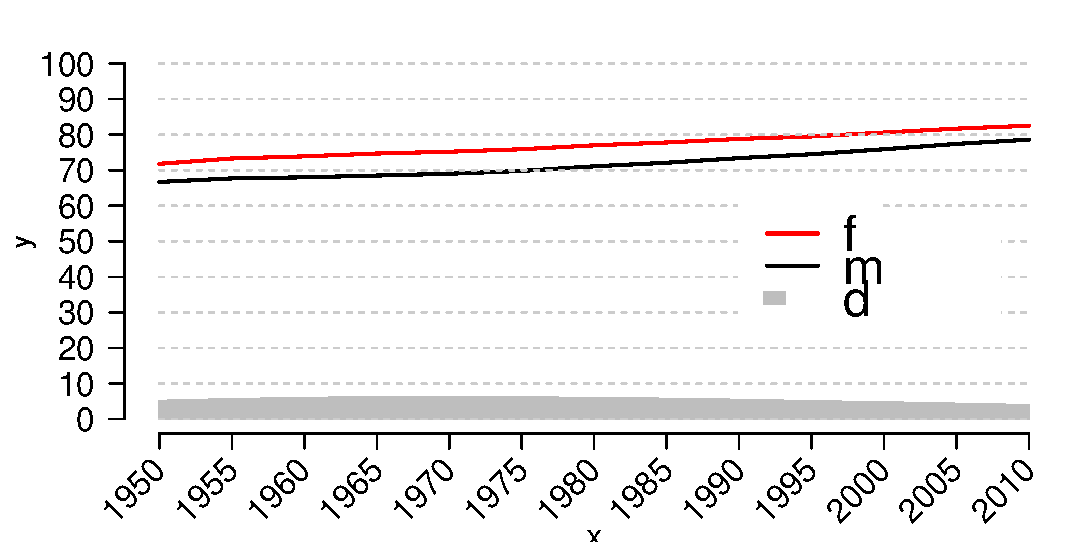
\includegraphics[width=\textwidth]{../figures/Fig2.1.eps}
\caption{Life expectancy at birth for males and females in the United Kingdom, 1950-2010 and life expectancy gender difference. Source: \cite{HMD2015}}
\label{Fig:07}
\end{figure}

Figure \ref{Fig:07} shows how life expectancy at birth in the UK has been changing over time. Life expectancy been steadily increasing, with men gaining 2.38 months per year over the past 60 years, and women slightly less at 2.14 months per year. The gender difference was largest during the late 60s, when it stood at over 6 years, but has been narrowing since then, and is currently under 4 years.


\begin{table}[hbtp!]
\caption{Life expectancy at birth for males and females in the United Kingdom, 1950-2010 and life expectancy gender difference (See Figure \ref{Fig:07}). Source: \cite{HMD2015}.}\label{Tab:07}
\centering
\bigskip
\begin{tabular}{>{\small}l<{\hspace{-6pt}}>{\small}r<{\hspace{-6pt}}>{\small}r<{\hspace{-6pt}}>{\small}r<{\hspace{-6pt}}>{\small}r<{\hspace{-6pt}}>{\small}r<{\hspace{-6pt}}>{\small}r<{\hspace{-6pt}}>{\small}r<{\hspace{-6pt}}>{\small}r<{\hspace{-6pt}}>{\small}r<{\hspace{-6pt}}>{\small}r<{\hspace{-6pt}}>{\small}r<{\hspace{-6pt}}>{\small}r<{\hspace{-6pt}}>{\small}r<{\hspace{-6pt}}}
  \hline
\emph{Year} & 1950 & 1955 & 1960 & 1965 & 1970& 1975 & 1980 & 1985 & 1990 & 1995 & 2000 & 2005 & 2010 \\
  \hline
  \emph{Males} & 66.70 & 67.70 & 68.00 & 68.50 & 69.00 & 69.80 & 71.10 & 72.10 & 73.40 & 74.50 & 75.90 & 77.40 & 78.60 \\ 
 \emph{Females} & 71.80 & 73.30 & 73.90 & 74.70 & 75.20 & 75.90 & 77.00 & 77.80 & 78.80 & 79.50 & 80.60 & 81.70 & 82.50 \\ 
\emph{Diff} & 5.10 & 5.60 & 5.90 & 6.20 & 6.20 & 6.10 & 5.90 & 5.70 & 5.40 & 5.00 & 4.70 & 4.30 & 3.90 \\ 
   \hline
\end{tabular}
\end{table}


\clearpage
\subsection{Life Expectancy at 65 and 80}

\begin{figure}[hbtp!]
\psfrag{y}[c][c]{\small{\emph{Remaining life expectancy}}}
\psfrag{x}[c][c]{\small{\emph{Year}}}
\psfrag{2010}[r][r]{\small{2010}}
\psfrag{2000}[r][r]{\small{2000}}
\psfrag{1990}[r][r]{\small{1990}}
\psfrag{1980}[r][r]{\small{1980}}
\psfrag{1970}[r][r]{\small{1970}}
\psfrag{1965}[r][r]{\small{1965}}
\psfrag{2005}[r][r]{\small{2005}}
\psfrag{1995}[r][r]{\small{1995}}
\psfrag{1985}[r][r]{\small{1985}}
\psfrag{1975}[r][r]{\small{1975}}
\psfrag{1960}[r][r]{\small{1960}}
\psfrag{1950}[r][r]{\small{1950}}
\psfrag{1955}[r][r]{\small{1955}}
\psfrag{1960}[r][r]{\small{1960}}
\psfrag{a}[l][l]{$e_{65}$ \emph{males}}
\psfrag{b}[l][l]{$e_{65}$ \emph{females}}
\psfrag{c}[l][l]{$e_{80}$ \emph{males}}
\psfrag{d}[l][l]{$e_{80}$ \emph{females}}
\psfrag{0}[r][r]{\small{0}}
\psfrag{10}[r][r]{\small{10}}
\psfrag{20}[r][r]{\small{20}}
\psfrag{5}[r][r]{\small{5}}
\psfrag{15}[r][r]{\small{15}}
\psfrag{25}[r][r]{\small{25}}
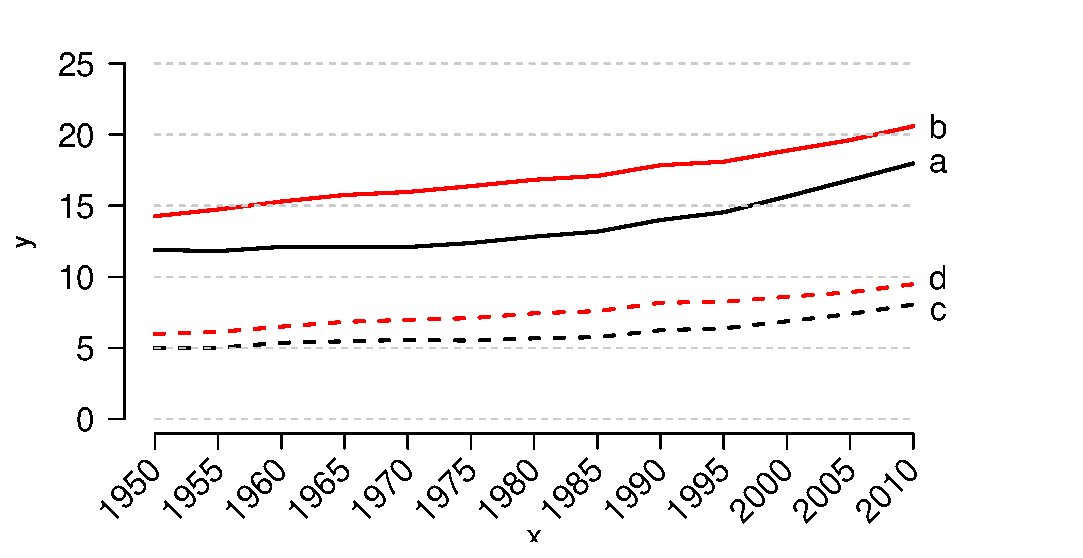
\includegraphics[width=\textwidth]{../figures/Fig2.2.eps}
\caption{Remaining life expectancy at ages 65 and 80 for males and females in the United Kingdom, 1950-2010. Source:  \cite{HMD2015}}
\label{Fig:08}
\end{figure}

Figure \ref{Fig:08} charts the trends in life expectancy at ages 65 and 80 in the UK. For both age groups women's life expectancy has increased slightly faster over the whole period, with 65-year-old women gaining  6.32 years as opposed to 6.08 for men, and 80-year-old women gaining  3.5 years compared to the 3.05 years gained by men over the past 60 years. The gender differential has however been decreasing from the late 1970s (for 65-year-olds) and the early 1990s (for 80-year-olds) in a similar fashion as overall life expectancy shown above. 

\begin{table}[hbtp!]
\caption{Remaining life expectancy at ages 65 and 80 for males and females in the United Kingdom, 1950-2010 (see Figure \ref{Fig:08}). Source: \cite{HMD2015}.}\label{Tab:22}
\centering

\bigskip
\begin{tabular}{>{\small\hspace{-8pt}}l<{\hspace{-6pt}}>{\small}r<{\hspace{-6pt}}>{\small}r<{\hspace{-6pt}}>{\small}r<{\hspace{-6pt}}>{\small}r<{\hspace{-6pt}}>{\small}r<{\hspace{-6pt}}>{\small}r<{\hspace{-6pt}}>{\small}r<{\hspace{-6pt}}>{\small}r<{\hspace{-6pt}}>{\small}r<{\hspace{-6pt}}>{\small}r<{\hspace{-6pt}}>{\small}r<{\hspace{-6pt}}>{\small}r<{\hspace{-6pt}}>{\small}r<{\hspace{-6pt}}}
  \hline
\emph{Year} & 1950 & 1955 & 1960 & 1965 & 1970& 1975 & 1980 & 1985 & 1990 & 1995 & 2000 & 2005 & 2010 \\
 \hline
$e_{65}$ \emph{males}&  11.90 & 11.81 & 12.11 & 12.12 & 12.10 & 12.38 & 12.83 & 13.18 & 14.00 & 14.54 & 15.65 & 16.81 & 17.98 \\ 
$e_{65}$ \emph{females} & 14.27 & 14.74 & 15.30 & 15.76 & 15.97 & 16.38 & 16.83 & 17.10 & 17.85 & 18.10 & 18.88 & 19.62 & 20.59 \\ 
$e_{80}$ \emph{males}  &5.01 & 5.01 & 5.37 & 5.47 & 5.57 & 5.52 & 5.68 & 5.76 & 6.25 & 6.38 & 6.88 & 7.39 & 8.06 \\ 
 $e_{80}$ \emph{females}& 5.99 & 6.13 & 6.50 & 6.84 & 6.98 & 7.10 & 7.44 & 7.59 & 8.18 & 8.25 & 8.60 & 8.92 & 9.49 \\ 
   \hline
\end{tabular}
\end{table}

\clearpage
\subsection{Survivorship at Young and Old Ages}

 
\begin{figure}[hbtp!]

\psfrag{a}[l][l]{\emph{I(0,15)}}
\psfrag{b}[l][l]{\emph{I(60,75)}}
\psfrag{y}[c][c]{\small{\emph{Proportion surviving}}}
\psfrag{x}[c][c]{\small{\emph{Year}}}
\psfrag{0.0}[r][r]{\small{0.0}}
\psfrag{0.2}[r][r]{\small{0.2}}
\psfrag{0.4}[r][r]{\small{0.4}}
\psfrag{0.6}[r][r]{\small{0.6}}
\psfrag{0.8}[r][r]{\small{0.8}}
\psfrag{1.0}[r][r]{\small{1.0}}
\psfrag{1.2}[r][r]{\small{1.2}}

\psfrag{A}[r][r]{\scriptsize{1922-24}}
\psfrag{B}[r][r]{\scriptsize{1925-29}}
\psfrag{C}[r][r]{\scriptsize{1930-34}}
\psfrag{D}[r][r]{\scriptsize{1935-39}}
\psfrag{E}[r][r]{\scriptsize{1940-44}}
\psfrag{F}[r][r]{\scriptsize{1945-49}}
\psfrag{G}[r][r]{\scriptsize{1950-54}}
\psfrag{H}[r][r]{\scriptsize{1955-59}}
\psfrag{I}[r][r]{\scriptsize{1960-64}}
\psfrag{J}[r][r]{\scriptsize{1965-69}}
\psfrag{K}[r][r]{\scriptsize{1970-74}}
\psfrag{L}[r][r]{\scriptsize{1975-79}}
\psfrag{M}[r][r]{\scriptsize{1980-84}}
\psfrag{N}[r][r]{\scriptsize{1985-89}}
\psfrag{O}[r][r]{\scriptsize{1990-94}}
\psfrag{P}[r][r]{\scriptsize{1995-9}}
\psfrag{Q}[r][r]{\scriptsize{2000-04}}
\psfrag{R}[r][r]{\scriptsize{2005-09}}
\psfrag{S}[r][r]{\scriptsize{2010-14}}
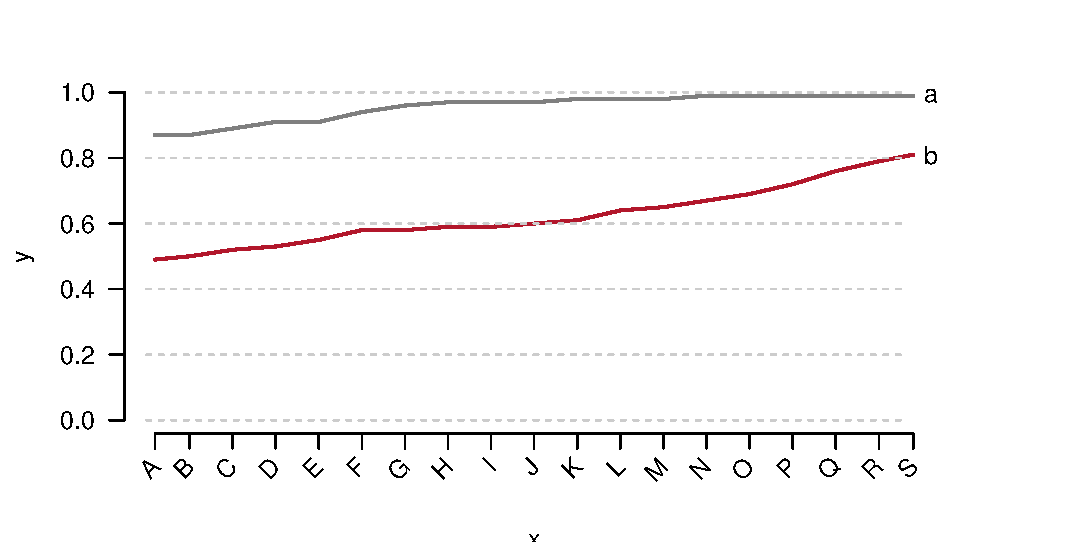
\includegraphics[width=\textwidth]{../figures/Fig2.3.eps}

\caption{Survival from birth to age 15 and from age 60 to age 75 years, United Kingdom, 1922-2011, both sexes combined. Source: own calculations from the Human Mortality Database \citep{Lees2014}}
\label{Fig:9}
\end{figure}
Figure \ref{Fig:9} shows survivorship from birth to age 15 and from 60 to 75 years in the UK for both sexes combined. Up until around 1950, the gradient of the two curves is similar, but from 1950 to the present day, survivorship from birth to age 15 has stagnated (simply because survivorship is asymptoting unity which corresponds to 100 per cent survival over the first 15 years of life) while survivorship from age 60 to age 75 years continues to improve. Currently, 81 per cent of 60-year-olds survive to age 75 years – and 92 per cent of a birth cohort survives to age 60 years.

\renewcommand{\arraystretch}{1.}

\begin{table}[hbtp!]
\caption{Survival from birth to age 15 and from age 60 to age 75 years, United Kingdom, 1922-2011, both sexes combined (see Figure \ref{Fig:9}). Source: own calculations from the Human Mortality Database \citep{Lees2014}.}
\centering
\begin{tabularx}\textwidth{>{\centering\arraybackslash\em\small}p{2cm} *2{>{\centering\arraybackslash\small}X}@{} >{\centering\arraybackslash\em\small}p{2cm} *2{>{\centering\arraybackslash\small}X}@{}}

  \hline
Years &\emph{I(0,15)} &\emph{ I(60,75) }& Years & \emph{I(0,15)}& \emph{I(60,75)} \\ 
  \hline
1922-24 & 0.87 & 0.49 & 1970-74 & 0.98 & 0.61 \\ 
  1925-29 & 0.87 & 0.50 & 1975-79 & 0.98 & 0.64 \\ 
  1930-34 & 0.89 & 0.52 & 1980-84 & 0.98 & 0.65 \\ 
  1935-39 & 0.91 & 0.53 & 1985-89 & 0.99 & 0.67 \\ 
  1940-44 & 0.91 & 0.55 & 1990-94 & 0.99 & 0.69 \\ 
  1045-49 & 0.94 & 0.58 & 1995-99 & 0.99 & 0.72 \\ 
  1950-54 & 0.96 & 0.58 & 2000-04 & 0.99 & 0.76 \\ 
  1955-59 & 0.97 & 0.59 & 2005-09 & 0.99 & 0.79 \\ 
  1960-64 & 0.97 & 0.59 & 2010-11 & 0.99 & 0.81 \\ 
  1965-69 & 0.97 & 0.60 &  &  &  \\ 
   \hline
\end{tabularx}
\end{table}

\clearpage

\subsection{Projected Life Expectancy at Birth}


\begin{figure}[hbtp!]
\psfrag{2012}[r][r]{\small{2012}}
\psfrag{2015}[r][r]{\small{2015}}
\psfrag{2020}[r][r]{\small{2020}}
\psfrag{2030}[r][r]{\small{2030}}
\psfrag{2040}[r][r]{\small{2040}}
\psfrag{2050}[r][r]{\small{2050}}
\psfrag{2025}[r][r]{\small{2025}}
\psfrag{2035}[r][r]{\small{2035}}
\psfrag{2045}[r][r]{\small{2045}}
\psfrag{f}[lB][lB]{\small{\emph{Females}}}
\psfrag{m}[lB][lB]{\small{\emph{Males}}}
\psfrag{d}[lB][lB]{\small{\emph{Difference}}}
\psfrag{y}[c][c]{\small{\emph{Life expectancy}}}
\psfrag{x}[c][c]{\small{\emph{Year}}}
\psfrag{0}[r][r]{\small{0}}
\psfrag{10}[r][r]{\small{10}}
\psfrag{20}[r][r]{\small{20}}
\psfrag{30}[r][r]{\small{30}}
\psfrag{90}[r][r]{\small{90}}
\psfrag{80}[r][r]{\small{80}}
\psfrag{70}[r][r]{\small{70}}
\psfrag{60}[r][r]{\small{60}}
\psfrag{50}[r][r]{\small{50}}
\psfrag{40}[r][r]{\small{40}}
\psfrag{30}[r][r]{\small{30}}
\psfrag{20}[r][r]{\small{20}}
\psfrag{100}[r][r]{\small{100}}

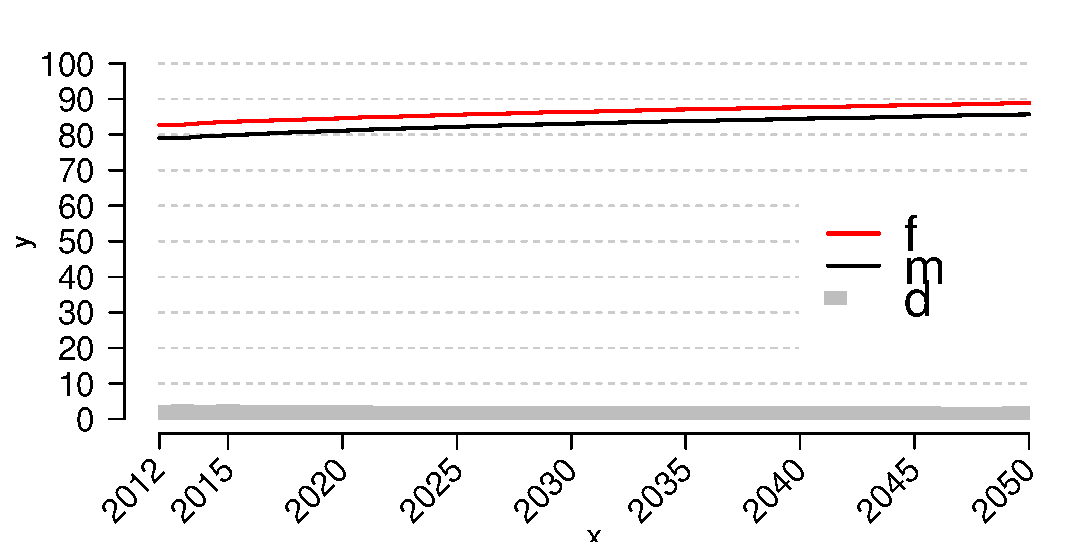
\includegraphics[width=\textwidth]{../figures/Fig2.4.eps}
\caption{Life expectancy at birth for males and females in the United Kingdom, 2012-2050 and life expectancy gender difference. Source: \cite{ONS2013c}.}
\label{Fig:10}
\end{figure}

The increasing trends in life expectancy are projected to continue to the middle of the 21st century (and beyond), with life expectancies at birth reaching 86 years for males and 89 years for females, and with the gender difference declining further to around 3 years. 



\begin{table}[hbtp!]
\caption{Life expectancy at birth for males and females in the United Kingdom, 2012-2050 and life expectancy gender difference (see for Figure \ref{Fig:10}). Source: \cite{ONS2013c}.}\label{Tab:10}
\centering
\bigskip
\renewcommand{\arraystretch}{1.2}

\begin{tabularx}\textwidth{p{2cm} *9{>{\centering\arraybackslash}X}@{}}
\hline
\emph{Year}  & 2012 & 2015 & 2020 & 2025 & 2030 & 2035& 2040 & 2045 & 2050 \\ 
\hline
  \emph{Males} &  79.00 & 79.80 & 81.10 & 82.20 & 83.10 & 83.80 & 84.50 & 85.10 & 85.70 \\ 
 \emph{Females} &  82.70 & 83.60 & 84.60 & 85.60 & 86.40 & 87.10 & 87.70 & 88.30 & 88.90 \\ 
\emph{Diff} &  3.70 & 3.80 & 3.50 & 3.40 & 3.30 & 3.30 & 3.20 & 3.20 & 3.20 \\ 
   \hline
\end{tabularx}
\end{table}

\clearpage
\subsection{Projected Life Expectancy at 65 and 80}

\begin{figure}[hbtp!]
\psfrag{y}[c][c]{\small{\emph{Remaining life expectancy}}}
\psfrag{x}[c][c]{\small{\emph{Year}}}
\psfrag{2012}[r][r]{\small{2012}}
\psfrag{2015}[r][r]{\small{2015}}
\psfrag{2020}[r][r]{\small{2020}}
\psfrag{2030}[r][r]{\small{2030}}
\psfrag{2040}[r][r]{\small{2040}}
\psfrag{2050}[r][r]{\small{2050}}
\psfrag{2025}[r][r]{\small{2025}}
\psfrag{2035}[r][r]{\small{2035}}
\psfrag{2045}[r][r]{\small{2045}}
\psfrag{a}[l][l]{$e_{65}$ \emph{males}}
\psfrag{b}[l][l]{$e_{65}$ \emph{females}}
\psfrag{c}[l][l]{$e_{80}$ \emph{males}}
\psfrag{d}[l][l]{$e_{80}$ \emph{females}}
\psfrag{0}[r][r]{\small{0}}
\psfrag{10}[r][r]{\small{10}}
\psfrag{20}[r][r]{\small{20}}
\psfrag{5}[r][r]{\small{5}}
\psfrag{15}[r][r]{\small{15}}
\psfrag{25}[r][r]{\small{25}}
\psfrag{30}[r][r]{\small{30}}

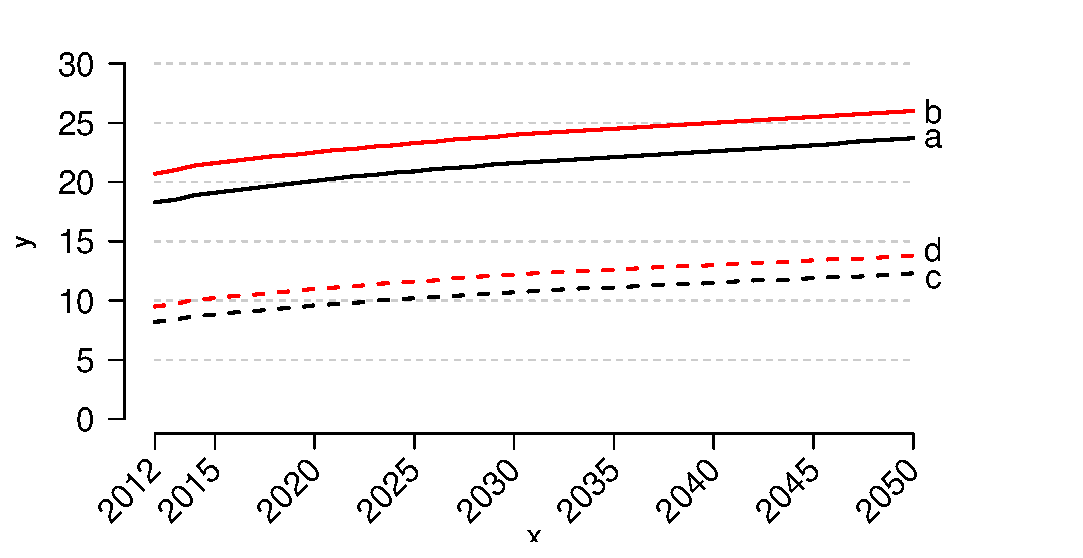
\includegraphics[width=\textwidth]{../figures/Fig2.5.eps}
\caption{Life expectancy at ages 65 and 80 for males and females in the United Kingdom, 2012-2050. Source: \cite{ONS2013c}}
\label{Fig:11}
\end{figure}

By 2050, life expectancy at age 65 is expected to reach 24 years for males and 26 years for females, while at age 80, life expectancies will have reached 12 and 14 years for males and females respectively. By 2050, life expectancies at age 80 will be at levels observed at age 65 years in the early 1980s, while life expectancies at age 65 in 2050 will correspond to those observed at age 50-55 years in early 1980s. 

\begin{table}[hbtp!]
\caption{Life expectancy at ages 65 and 80 for males and females in the United Kingdom, 2012-2050 (see Figure \ref{Fig:11}). Source: \cite{ONS2013c}.}\label{Tab:21}
\centering
\bigskip
\renewcommand{\arraystretch}{1.2}

\begin{tabularx}\textwidth{p{2cm} *9{>{\centering\arraybackslash}X}@{}}
\hline
\emph{Year}  & 2012 & 2015 & 2020 & 2025 & 2030 & 2035& 2040 & 2045 & 2050 \\ 
\hline
$e_{65}$ \emph{males} & 18.30 & 19.10 & 20.10 & 20.90 & 21.60 & 22.10 & 22.60 & 23.10 & 23.70 \\ 
$e_{65}$ \emph{females} &  20.70 & 21.60 & 22.50 & 23.30 & 24.00 & 24.50 & 25.00 & 25.50 & 26.00 \\ 
$e_{80}$ \emph{males} &  8.20 & 8.80 & 9.60 & 10.20 & 10.70 & 11.10 & 11.50 & 11.90 & 12.30 \\ 
$e_{80}$ \emph{females} &  9.50 & 10.20 & 11.00 & 11.60 & 12.20 & 12.60 & 13.00 & 13.40 & 13.80 \\ 
\hline
\end{tabularx}
\end{table}


\clearpage
\subsection{Projected Cohort Life Expectancies}

\begin{figure}[hbtp!]
\psfrag{b}[cc][cr]{\small{2012}}
\psfrag{d}[cc][cr]{\small{2050}}
\psfrag{aa}[c][c]{\small{\emph{Attained age}}}

\psfrag{A}[r][l]{\small{0}}
\psfrag{B}[r][l]{\small{20}}
\psfrag{C}[r][l]{\small{40}}
\psfrag{D}[r][l]{\small{60}}
\psfrag{E}[r][l]{\small{65}}
\psfrag{F}[r][l]{\small{75}}
\psfrag{G}[r][l]{\small{80}}
\psfrag{H}[r][l]{\small{85}}
\psfrag{LE}[c][c]{\small{\emph{Life expectancy}}}

\psfrag{xx}{\small{\emph{Males}}}
\psfrag{yy}{\small{\emph{Females}}}
\psfrag{0}[r][r]{\small{0}}
\psfrag{20}[r][r]{\small{20}}
\psfrag{40}[r][r]{\small{40}}
\psfrag{60}[r][r]{\small{60}}
\psfrag{80}[r][r]{\small{80}}
\psfrag{100}[r][r]{\small{100}}
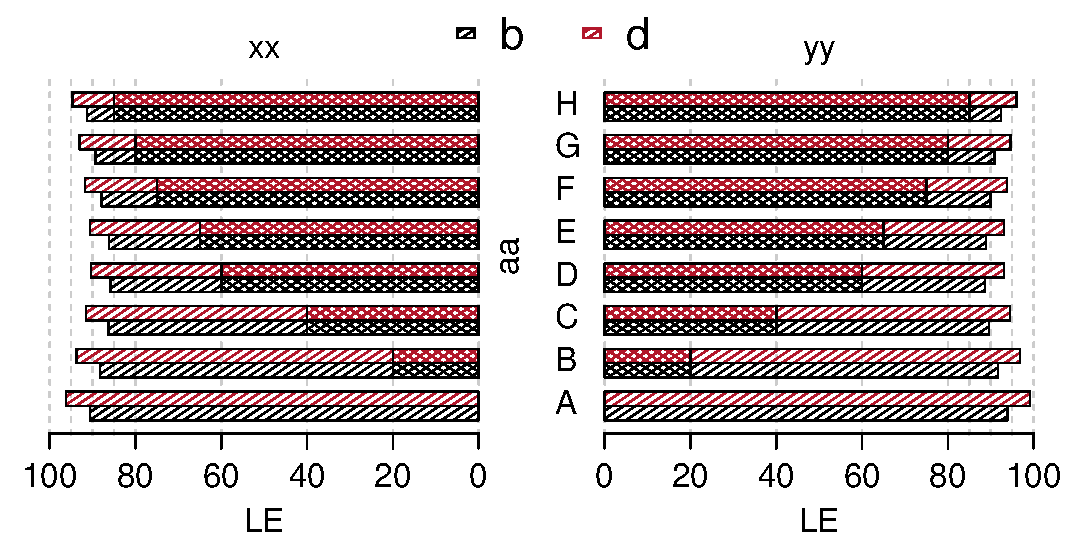
\includegraphics[width=\textwidth]{../figures/Fig2.6.eps}
\caption{Cohort life expectancies in 2012 and 2050 for selected cohorts, principal projection, 2012-based. Source: \cite{ONS2013c} }
\label{Fig:26}
\end{figure}

As opposed to the \emph{period} life expectancies described in the previous two charts, the \emph{cohort} life expectancies shown in Figure \ref{Fig:26} are about 10 years higher at birth for both males and females.  This is because cohort measures take into account predicted future improvements in mortality rates. A baby born in 2012 is therefore expected to live until the age of 90.6 if he is a boy or 93.90 if she is a girl. Babies born in 2050 can expect to live almost 6 years longer.  
   

\begin{table}[hbtp!]
\caption{Cohort life expectancies in 2012 and 2050 for selected cohorts, principal projection, 2012-based (see Figure \ref{Fig:26}). Source: \cite{ONS2013c}.}\label{Tab:26}
\vspace{1ex}

\centering
\begin{tabularx}\textwidth{p{1.8cm} p{1.5cm} *8{>{\centering\arraybackslash}X}@{}}
\hline 

 &  & $e_{0}$& $e_{20}$ &$e_{40}$ &$e_{60}$ &$e_{65}$ &$e_{75}$ & $e_{80}$ & $e_{85}$ \\ 
  \hline
\multirow{2}{*}{\emph{Males}} & 2012 & 90.60 & 68.30 & 46.30 & 25.80 & 21.20 & 12.90 & 9.30 & 6.30 \\ 
  & 2050 & 96.20 & 73.70 & 51.50 & 30.40 & 25.60 & 16.80 & 13.00 & 9.70 \\ 
  \\[-2ex]
\multirow{2}{*}{\emph{Females}} & 2012 & 93.90 & 71.70 & 49.60 & 28.70 & 23.90 & 15.00 & 10.90 & 7.40 \\ 
 & 2050 & 99.10 & 76.80 & 54.50 & 33.10 & 28.10 & 18.80 & 14.60 & 11.00 \\ 
   \hline
\end{tabularx}
\end{table}




\chapter{How healthy life expectancy is changing} %3

\subsection{Healthy and Disability-free Life Expectancies}


\begin{figure}[hbtp!]
\psfrag{2000}[r][r]{\small{2000-02}}
\psfrag{2001}[r][r]{\small{2001-03}}
\psfrag{2002}[r][r]{\small{2002-04}}
\psfrag{2003}[r][r]{\small{2003-05}}
\psfrag{2004}[r][r]{\small{2004-06}}
\psfrag{2005}[r][r]{\small{2005-07}}
\psfrag{2006}[r][r]{\small{2006-08}}
\psfrag{2007}[r][r]{\small{2007-09}}
\psfrag{2008}[r][r]{\small{2008-10}}
\psfrag{2009}[r][r]{\small{2009-11}}
\psfrag{y}[c][c]{\small{Life expectancy}}
\psfrag{x}[c][c]{\small{Years}}

\psfrag{a}[Bl][Bl]{\small{LE \emph{males}}}
\psfrag{b}[Bl][Bl]{\small{HLE \emph{males}}}
\psfrag{c}[Bl][Bl]{\small{DFLE \emph{males}}}
\psfrag{d}[Bl][Bl]{\small{LE \emph{females}}}
\psfrag{e}[Bl][Bl]{\small{HLE \emph{females}}}
\psfrag{f}[Bl][Bl]{\small{DFLE \emph{females}}}
\psfrag{0}[r][r]{\small{0}}
\psfrag{40}[r][r]{\small{40}}
\psfrag{20}[r][r]{\small{20}}
\psfrag{60}[r][r]{\small{60}}
\psfrag{80}[r][r]{\small{80}}

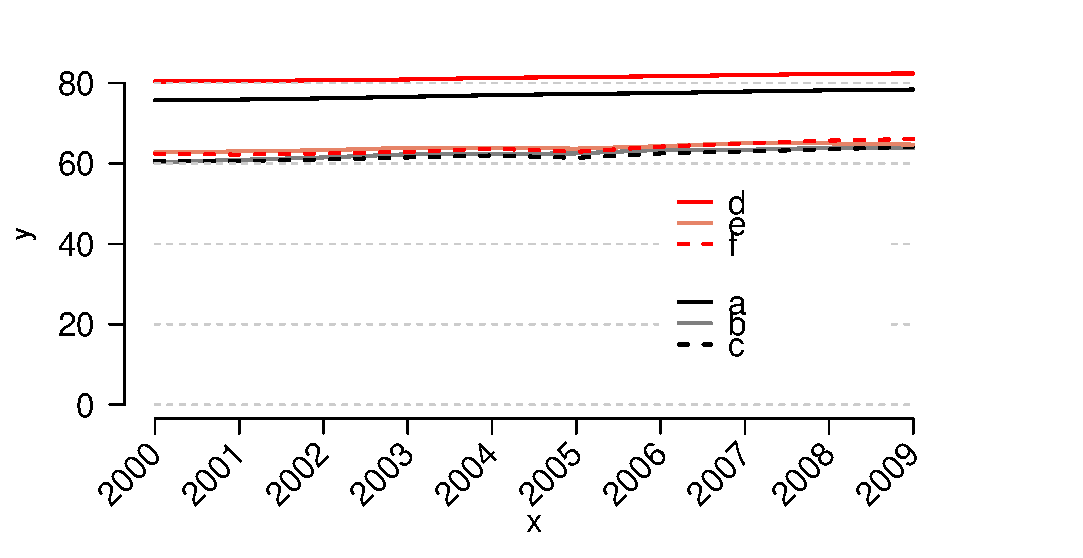
\includegraphics[width=\textwidth]{../figures/Fig3.1.eps}
\caption{Life expectancy (LE), healthy life expectancy (HLE) and disability-free life expectancy (DFLE) at birth in the United Kingdom, 2000-02 to 2009-11, males and females. Source: \cite{ONS2012}.}
\label{Fig:31}
\end{figure}



As life expectancy increases as discussed above, health expectancies enable us to determine whether these `extra' years lived are spent in good health or free from a limiting illness or disability. The development in life expectancy, healthy life expectancy and disability-free life expectancy at birth for the United Kingdom for the period 2000-02 to 2009-11 is shown in Figure \ref{Fig:31} which reveals over this period that healthy life expectancy at birth increased in absolute terms more than life expectancy for males and females, which would suggest a compression of morbidity. While this is also observed for disability-free life expectancy at birth for males, it is not the case for females.  

Gender differences in life expectancy are generally greater than the gender differences in both healthy life expectancy and disability-free life expectancy, which would suggest that most of the increase in life expectancy for females is with disability or in not good health.  


\begin{table}[hpbt!]

\centering
\caption{Life expectancy (LE), healthy life expectancy (HLE) and disability-free life expectancy (DFLE) at birth in the United Kingdom, 2000-02 to 2009-11, males and females (see Figure \ref{Fig:31}). Source: \cite{ONS2012}.}
\vspace{1ex}

\begin{tabularx}\textwidth{X X X X X}
\hline
 & & 	LE	&	HLE		& DFLE \\
 \hline
 
\multirow{10}{*}{Males	} &	2000-02	&	75.7	&	60.7	&	60.3\\
		&2001-03		&	75.9	&	60.6	&	60.9	\\	
		
&		2002-04	&		76.2	&	61.0	&	61.5\\
&		2003-05	&		76.6	&	61.5	&	62.3\\
&		2004-06	&		77.0	&	62.0	&	62.4\\
& 		2005-07	&		77.3	&	61.4	&	62.5\\
&		2006-08	&		77.5	&	62.5	&	63.4\\
&		2007-09	&		77.9	&	63.0	&	63.4\\
&		2008-10	&		78.2	&	63.5	&	63.9\\
&		2009-11	&		78.4	&	64.2&	63.9\\
\hline		
\multirow{10}{*}{Females	}&2000-02	&		80.4		&62.4&		62.8\\
&		2001-03&			80.5	&	62.2	&	63.0	\\	
&		2002-04	&		80.7	&	62.5	&	63.3\\
&		2003-05	&		80.9	&	62.9	&	63.9\\
&		2004-06	&		81.3	&	63.7	&	63.9\\
&		2005-07	&		81.5	&	62.9	&	63.7\\
&		2006-08	&		81.7	&	64.2	&	64.3\\
&		2007-09	&		82.0	&	65.0	&	65.1\\
&		2008-10	&		82.3	&	65.7	&	65.0\\
&		2009-11	&		82.4&	66.1&	64.7\\
\hline

\end{tabularx}
\vspace{0.5ex}

\raggedleft \footnotesize{Estimates are based on a three year moving average.}
\end{table}
\clearpage		


%



\chapter{Dependency ratios; and population over 65} %4
\subsection{Median Age}

\begin{figure}[hbtp!]
\psfrag{2014}[r][r]{\small{2014}}
\psfrag{2010}[r][r]{\small{2010}}
\psfrag{2006}[r][r]{\small{2006}}
\psfrag{2002}[r][r]{\small{2002}}
\psfrag{1998}[r][r]{\small{1998}}
\psfrag{1994}[r][r]{\small{1994}}
\psfrag{1990}[r][r]{\small{1990}}
\psfrag{1986}[r][r]{\small{1986}}
\psfrag{1982}[r][r]{\small{1982}}
\psfrag{1978}[r][r]{\small{1978}}
\psfrag{1974}[r][r]{\small{1974}}

\psfrag{ma}{\normalsize{\emph{Median age}}}
\psfrag{x}{\normalsize{\emph{Year}}}
\psfrag{30}{\small{30}}
\psfrag{32}{\small{32}}
\psfrag{34}{\small{34}}
\psfrag{36}{\small{36}}
\psfrag{38}{\small{38}}
\psfrag{40}{\small{40}}
\psfrag{42}{\small{42}}

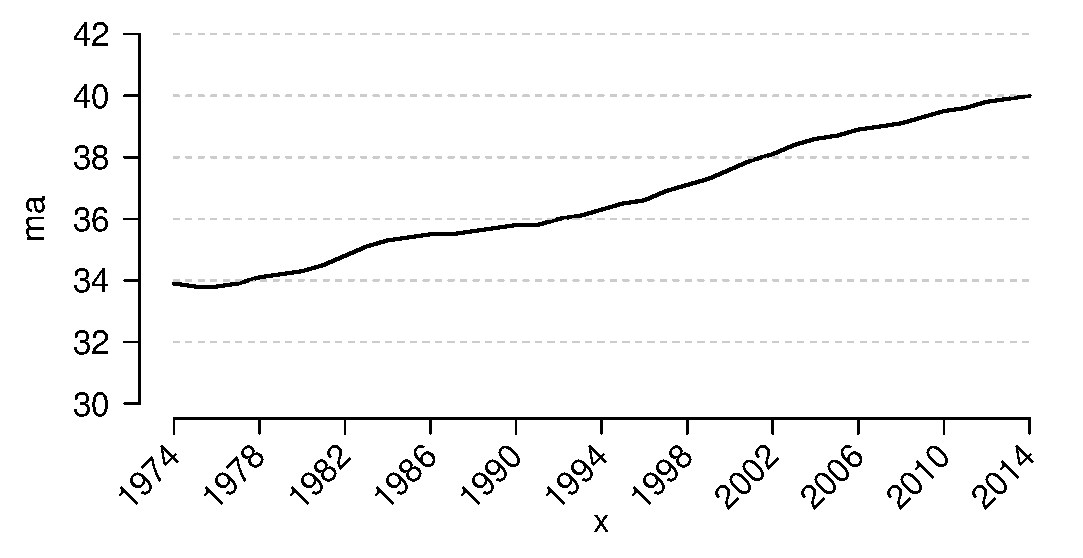
\includegraphics[width=\textwidth]{../figures/Fig4.1.eps}
\caption{Median age in the UK 1974 onwards. Source: \citet{ONS2015b}.}
\label{Fig:12}
\end{figure}

The population of the UK is ageing. Ageing of the population refers to both the increase in the average (median) age of the population and the increase in the number and proportion of older people in the population.
The median age of the UK population (that is the age at which half the population is younger and half the population is older) at mid-2014 was at its highest ever at 40.0. This is a slight increase from last year, caused by the growth in population at older ages. 
Over the 40 year period 1974 to 2014, the median age of the UK population has increased from 33.9 years to 40.0 years; an increase of over 6 years.

\renewcommand{\arraystretch}{1.2}

\begin{table}[hbtp!]
\centering
\caption{Median age in the UK 1974 onwards (see Figure \ref{Fig:12}). Source: \citet{ONS2015b}.}
\vspace{1ex}
\begin{tabularx}\textwidth{>{\small\hspace{-6pt}}p{1.6cm} *{11}{>{\centering\arraybackslash}X}@{}}
  \hline
\emph{Year}&1974 & 1978 & 1982 & 1986 & 1990 & 1994 & 1998 & 2002 & 2006 & 2010& 2014 \\ 
  \hline
\emph{Median Age}& 33.9 & 34.1 & 34.8 & 35.5 & 35.8 & 36.3 & 37.1 & 38.1 & 38.9 & 39.5 & 40.0 \\ 
   \hline
\end{tabularx}
\end{table}

\clearpage

\subsection{Proportion of people at older ages}
\begin{figure}[hbtp!]
\psfrag{y}[c][c]{\normalsize{\emph{Proportion of population}}}
\psfrag{x}[c][c]{\normalsize{\emph{Year}}}
\psfrag{2014}[r][r]{\small{2014}}
\psfrag{2010}[r][r]{\small{2010}}
\psfrag{2006}[r][r]{\small{2006}}
\psfrag{2002}[r][r]{\small{2002}}
\psfrag{1998}[r][r]{\small{1998}}
\psfrag{1994}[r][r]{\small{1994}}
\psfrag{1990}[r][r]{\small{1990}}
\psfrag{1986}[r][r]{\small{1986}}
\psfrag{1982}[r][r]{\small{1982}}
\psfrag{1978}[r][r]{\small{1978}}
\psfrag{1974}[r][r]{\small{1974}}

\psfrag{ma}{\normalsize{Median age}}
\psfrag{10}[r][r]{\small{10 \%}}
\psfrag{12}[r][r]{\small{12 \%}}
\psfrag{4}[r][r]{\small{4 \%}}
\psfrag{6}[r][r]{\small{6 \%}}
\psfrag{8}[r][r]{\small{8 \%}}
\psfrag{0}[r][r]{\small{0 \%}}
\psfrag{2}[r][r]{\small{2 \%}}

\psfrag{a}{\small{65 -- 74}}
\psfrag{b}{\small{75 -- 84}}
\psfrag{c}{\small{85 and over}}

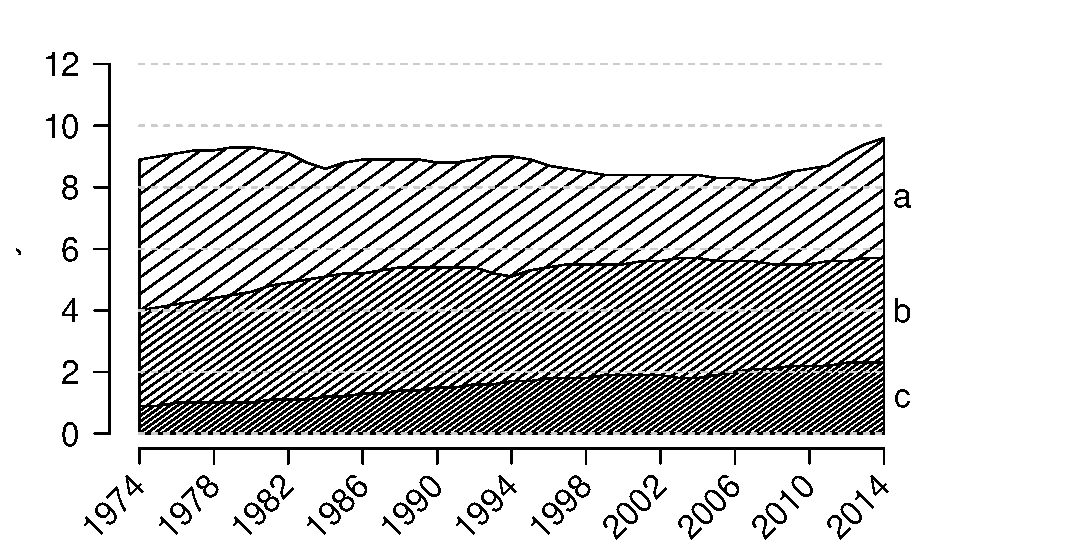
\includegraphics[width=\textwidth]{../figures/Fig4.2.eps}
\caption{Proportion of people at older ages, UK population mid-1974 onwards. Source: \citet{ONS2015b}.}
\label{Fig:13}
\end{figure}


In terms of increases in the number and proportion of older people in the UK population, the population aged 65 and over has grown by 47 \% since mid-1974 to make up nearly 18 \% of the total population in mid-2014 while the number of people aged 75 and over has increased by 89 \% over the period and now makes up 8 \% of the population (Figure \ref{Fig:13}). 


\begin{table}[hpbt!]
\renewcommand{\arraystretch}{0.89}
\centering
\caption{Proportion of people at older ages, UK population mid-1974 onwards (see Figure \ref{Fig:13}). Source: \citet{ONS2015b}.}\label{Tab:41}
\vspace{1ex}

\begin{tabularx}\textwidth{p{3cm} *4{>{\centering\arraybackslash}X}@{}}
 
\hline
 & \multicolumn{3}{l}{\emph{Age-group as percentage of total population}}	&  \\
 \hline
 \emph{Mid-Year} &\emph{ 65 -- 74 }& \emph{75 -- 84} & \emph{85 and over} & \emph{Median Age} \\ 
  \hline
1974 & 8.90 & 4.00 & 0.90 & 33.90 \\ 
  1975 & 9.00 & 4.10 & 0.90 & 33.80 \\ 

  1980 & 9.30 & 4.60 & 1.00 & 34.30 \\ 

  1985 & 8.80 & 5.20 & 1.20 & 35.40 \\ 

  1990 & 8.80 & 5.40 & 1.50 & 35.80 \\ 

  1995 & 8.90 & 5.30 & 1.70 & 36.50 \\ 

  2000 & 8.40 & 5.50 & 1.90 & 37.60 \\ 

  2005 & 8.30 & 5.60 & 1.90 & 38.70 \\ 

  2010 & 8.60 & 5.50 & 2.20 & 39.50 \\ 

  2014 & 9.60 & 5.70 & 2.30 & 40.00 \\ 
 
\hline
\end{tabularx}

\end{table}





\clearpage
\subsection{Projected Working and Pension Age Populations}

\begin{figure}[hbtp!]
\psfrag{2012}[r][r]{\small{2012}}
\psfrag{2015}[r][r]{\small{2015}}
\psfrag{2020}[r][r]{\small{2020}}
\psfrag{2025}[r][r]{\small{2025}}
\psfrag{2030}[r][r]{\small{2030}}
\psfrag{2035}[r][r]{\small{2035}}
\psfrag{2040}[r][r]{\small{2040}}
\psfrag{2041}[r][r]{\small{2041}}
\psfrag{m}{\small{Working age}}
\psfrag{f}{\small{Pension age}}
\psfrag{x}[c][c]{\normalsize{\emph{Year}}}
\psfrag{50}[r][r]{\small{50}}
\psfrag{40}[r][r]{\small{40}}
\psfrag{30}[r][r]{\small{30}}
\psfrag{20}[r][r]{\small{20}}
\psfrag{10}[r][r]{\small{10}}
\psfrag{0}[r][r]{\small{0}}
\psfrag{xx}[c][c]{\small{\emph{Population (in millions)}}}

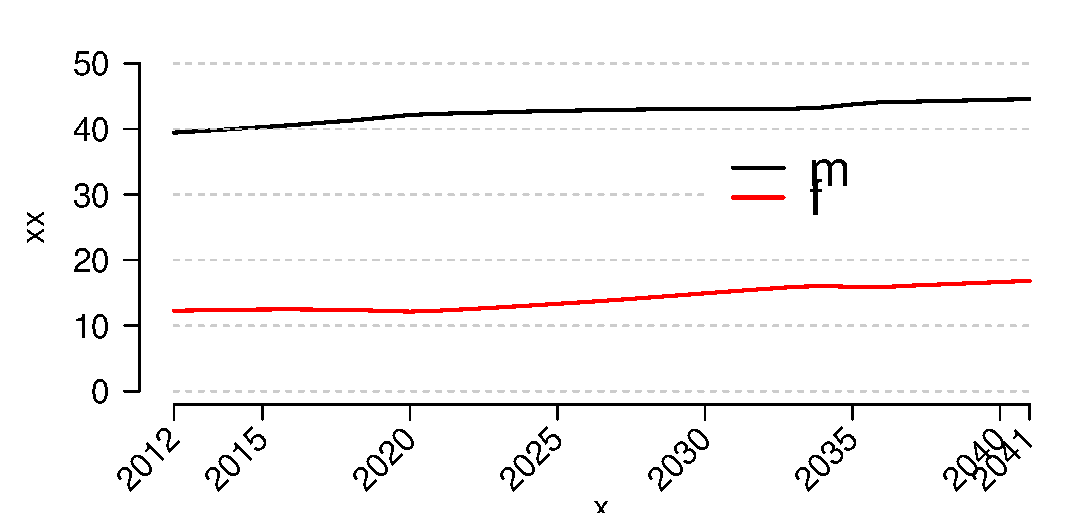
\includegraphics[width=\textwidth]{../figures/Fig4.3.eps}
\caption{Projections of working age and pensionable age population\protect \footnotemark, United Kingdom 2012-2041. Source: \cite{ONS2013c}.}
 
\label{Fig:14}
\end{figure}

The great majority of the predicted increase of the UK population over the coming decades is split almost equally between the working age and pension age age groups. In relative terms however, this translates to a lowering of the old age dependency ratio (or support ratio), which is the number of people of working age per person of pension age. Due to changes in the state pension age (SPA) the ratio will increase slightly for a few more years, and reach a maximum of 3.47 in 2020 before starting to fall, and is currently predicted to be 2.65 in 2041 unless further changes to the SPA are forthcoming. 


\footnotetext{Working age and pensionable age populations based on state pension age (SPA) for given year. Between 2012 and 2018, SPA will change from 65 years for men and 61 years for women, to 65 years for both sexes. Then between 2019 and 2020, SPA will change from 65 years to 66 years, and between 2034 and 2046 the SPA will increase in two stages from 66 years to 68 years for both sexes. }

\begin{table}[hpbt!]

\centering
\caption{Projections of working age and pensionable age population (in thousands); United Kingdom 2012-2041 (see Figure \ref{Fig:14}). Source: \cite{ONS2013c}.}\label{Tab:42}
\begin{tabularx}\textwidth{p{3cm} *3{>{\centering\arraybackslash}X}@{}}
\hline

 & \emph{Working age} & \emph{Pension age} & \emph{Old-age Dependency Ratio} \\ 
  \hline
  2012 & 39,441 & 12,280 & 3.21 \\ 
 
  2015 & 40,282 & 12,470 & 3.23 \\ 
 
  2020 & 42,145 & 12,146 & 3.47 \\ 

  2025 & 42,760 & 13,332 & 3.21 \\ 
  
  2030 & 43,028 & 14,932 & 2.88 \\ 

  2035 & 43,751 & 15,913 & 2.75 \\ 
 
  2041 & 44,563 & 16,837 & 2.65 \\ 
   \hline
   
   \end{tabularx}
\end{table}
\clearpage

\subsection{Old Age Dependency Ratio}

\begin{figure}[hbtp!]
\psfrag{2012}[r][r]{\small{2012}}
\psfrag{2015}[r][r]{\small{2015}}
\psfrag{2020}[r][r]{\small{2020}}
\psfrag{2025}[r][r]{\small{2025}}
\psfrag{2030}[r][r]{\small{2030}}
\psfrag{2035}[r][r]{\small{2035}}
\psfrag{2037}[r][r]{\small{2037}}
\psfrag{a}[r][r]{\small{\emph{\textcolor{red}{United Kingdom}}}}
\psfrag{b}[r][r]{\small{England}}
\psfrag{c}[r][r]{\small{Wales}}
\psfrag{d}[r][r]{\small{Scotland}}
\psfrag{e}[r][r]{\small{N. Ireland}}

\psfrag{x}[c][c]{\small{\emph{Year}}}
\psfrag{y}[c][c]{\small{\emph{Dependency Ratio}}}
\psfrag{2.2}[r][r]{\small{2.2}}
\psfrag{2.4}[r][r]{\small{2.4}}
\psfrag{2.6}[r][r]{\small{2.6}}
\psfrag{2.8}[r][r]{\small{2.8}}
\psfrag{3.0}[r][r]{\small{3.0}}
\psfrag{3.2}[r][r]{\small{3.2}}
\psfrag{3.4}[r][r]{\small{3.4}}
\psfrag{3.6}[r][r]{\small{3.6}}
\psfrag{3.8}[r][r]{\small{3.8}}
\psfrag{4.0}[r][r]{\small{4.0}}

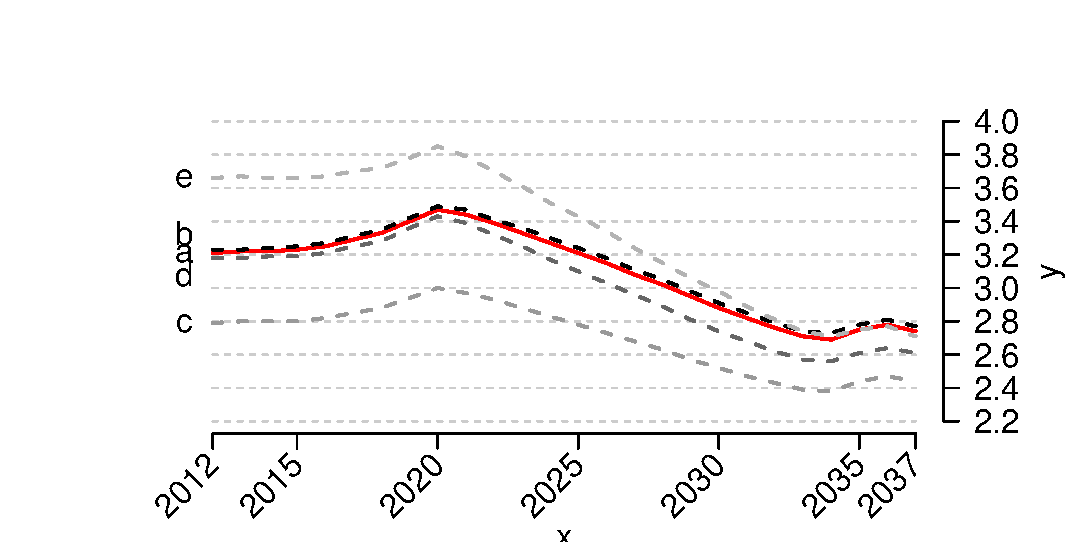
\includegraphics[width=\textwidth]{../figures/Fig4.4.eps}
\caption{Projected old-age dependency ratios, United Kingdom 2012-2037. Source: \cite{ONS2014b}.}
\label{Fig:15}
\end{figure}

The projected changes in the old age-dependency ratio for the UK and its constituent countries are shown in Figure \ref{Fig:15}, where the effects of the Pensions Act are clearly seen as the curves increase, before inevitably falling again.By 2037 the ration is projected to be 2.77 for England, 2.71 for Northern Ireland, 2.61 for Scotland and 2.44 for Wales.

\begin{table}[hpbt!]

\centering
\caption{Projected old-age dependency ratios, United Kingdom 2012-2037 (see Figure \ref{Fig:15}). Source: \cite{ONS2014b}.}\label{Tab:43}
\vspace{1ex}

\begin{tabularx}\textwidth{p{3cm} *5{>{\centering\arraybackslash}X}@{}}
\hline 
& United Kingdom & England & Wales & Scotland & Northern Ireland \\ 
  \hline
2012 & 3.21 & 3.23 & 2.79 & 3.18 & 3.66 \\ 
  2015 & 3.23 & 3.25 & 2.80 & 3.19 & 3.66 \\ 
  2020 & 3.47 & 3.49 & 3.00 & 3.43 & 3.85 \\ 
  2025 & 3.21 & 3.24 & 2.78 & 3.10 & 3.43 \\ 
  2030 & 2.88 & 2.91 & 2.52 & 2.74 & 2.98 \\ 
  2035 & 2.75 & 2.78 & 2.44 & 2.61 & 2.75 \\ 
  2037 & 2.74 & 2.77 & 2.44 & 2.61 & 2.71 \\ 
   \hline
\end{tabularx}
\end{table}

\chapter{Education, training and work} %5

\subsection{Sectoral employment by age group}

\begin{figure}[hbtp!]
\psfrag{a}[Br][Bl]{\small{18 -- 24}}
\psfrag{b}[Br][Bl]{\small{25 -- 49}}
\psfrag{c}[Br][Bl]{\small{50 -- 64}}
\psfrag{d}[Br][Bl]{\small{65 -- 69}}


\psfrag{1}[r][r]{\small{\emph{Finance}}}
\psfrag{2}[r][r]{\small{\emph{Construction}}}
\psfrag{3}[r][r]{\small{\emph{Manufacturing}}}
\psfrag{4}[r][r]{\small{\emph{Public Administration}}}
\psfrag{5}[r][r]{\small{\emph{Heanth \& Social care}}}
\psfrag{6}[r][r]{\small{\emph{Hospitality}}}
\psfrag{7}[r][r]{\small{\emph{Retail}}}
\psfrag{8}[r][r]{\small{\emph{Education}}}
\psfrag{9}[r][r]{\small{\emph{Transport}}}

\psfrag{10}[r][r]{\small{\emph{Other sectors}}}

\psfrag{0.0}[c][c]{\small{0 \%}}
\psfrag{0.2}[c][c]{\small{20 \%}}
\psfrag{0.4}[c][c]{\small{40 \%}}
\psfrag{0.6}[c][c]{\small{60 \%}}
\psfrag{0.8}[c][c]{\small{80 \%}}
\psfrag{1.0}[c][c]{\small{100 \%}}
\psfrag{x}[c][c]{\small{\emph{Proportion of workers}}}


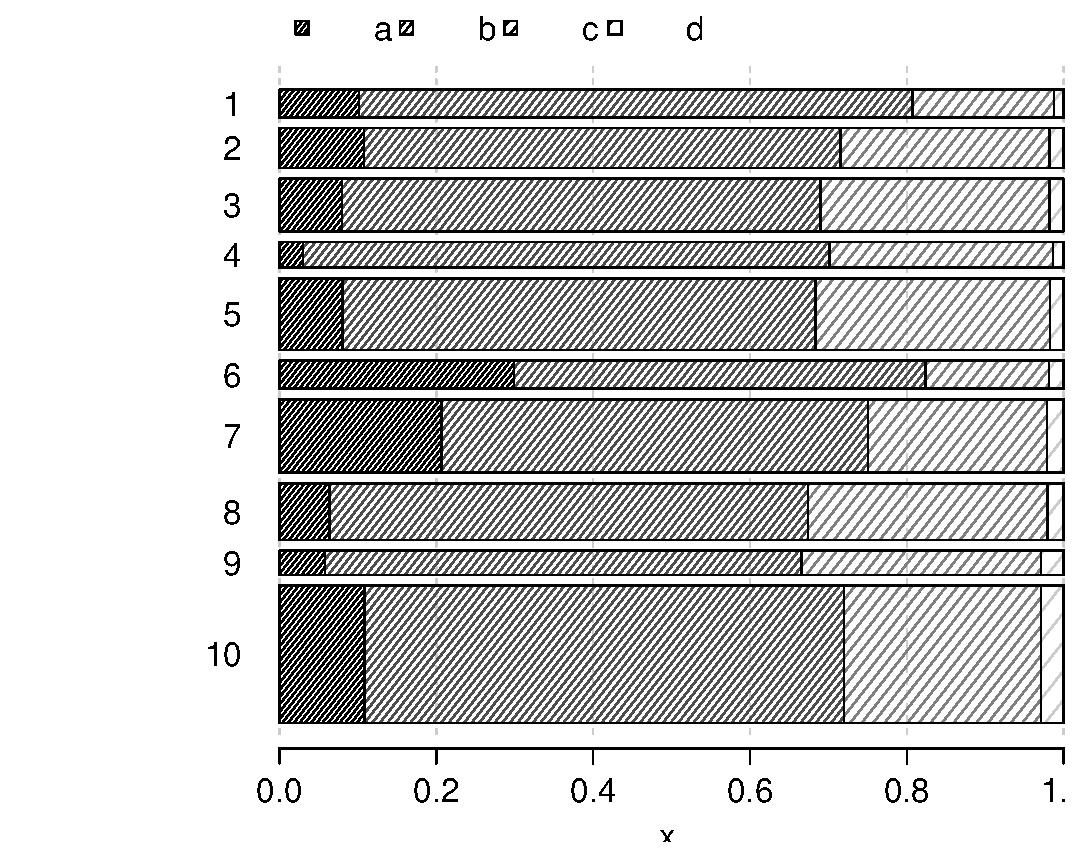
\includegraphics[width=\textwidth]{../figures/Fig5.1.eps}
\caption{Proportion of workers (empoyed and self-employed) by age group and sector, 2012, Labour Force Survey (LSF) representative sample of UK private households. Source: \cite{DWP2013}.}\label{Fig:51}
\end{figure}


Figure \ref{Fig:51} plots the proportion of workers in each age group by occupational sector. The width of each sector's bar is  furthermore proportional to the number of workers in each of them. The 50--64 and 65--69 age groups represent 35 \% of the population and have a similar representation in the Education and Transport sectors (around 33 \%); but are particularly under-represented in the Finance and Hospitality sectors (under 19 \%).


\begin{table}[hbtp!]

\caption{Proportion of workers (empoyed and self-employed) by age group and sector, 2012, LFS representative sample of UK private households -- \emph{row} percentages  (see Figure \ref{Fig:51}). Source: \cite{DWP2013}.}\label{Tab:51}
\centering
\begin{tabularx}\textwidth{l *5{>{}X<{\raggedleft \enspace \%}}@{}}
  \hline
   &\multicolumn{4}{c}{\emph{Age group}}\\
  \cline{2-6}
   & \multicolumn{1}{r}{18 -- 24} & 
   \multicolumn{1}{r}{25 -- 49} &
   \multicolumn{1}{r}{50 -- 64} &
   \multicolumn{1}{r}{65 -- 69}   & \multicolumn{1}{r}{18 -- 69}  \\ 
  \hline
\emph{Finance} & 10.15 & 70.57 & 18.06 & 1.22 & 100.00 \\ 
  \emph{Construction} & 10.77 & 60.75 & 26.69 & 1.79 & 100.00 \\ 
  \emph{Manufacturing} & 7.95 & 61.07 & 29.15 & 1.83 & 100.00 \\ 
  \emph{Public Administration} & 2.99 & 67.13 & 28.50 & 1.38 & 100.00 \\ 
  \emph{Health\& Social care} & 8.01 & 60.31 & 29.92 & 1.77 & 100.00 \\ 
  \emph{Hospitality} & 29.89 & 52.48 & 15.75 & 1.88 & 100.00 \\ 
  \emph{Retail} & 20.69 & 54.33 & 22.87 & 2.10 & 100.00 \\ 
  \emph{Education} & 6.40 & 61.00 & 30.57 & 2.03 & 100.00 \\ 
  \emph{Transport} & 5.83 & 60.76 & 30.54 & 2.87 & 100.00 \\ 
  \emph{Other sectors} & 10.84 & 61.16 & 25.09 & 2.91 & 100.00 \\ 
   \hline
\end{tabularx}
\end{table}

\begin{table}[hbtp!]

\caption{Proportion of workers (empoyed and self-employed) by age group and sector, 2012, LFS representative sample of UK private households -- \emph{column} percentages  (see Figure \ref{Fig:51}). Source: \cite{DWP2013}.}\label{Tab:53}
\centering
\begin{tabularx}\textwidth{l *5{>{}X<{\raggedleft \enspace \%}}@{}}
  \hline
   &\multicolumn{4}{c}{\emph{Age group}}\\
  \cline{2-6}
   & \multicolumn{1}{r}{18 -- 24} & 
   \multicolumn{1}{r}{25 -- 49} &
   \multicolumn{1}{r}{50 -- 64} &
   \multicolumn{1}{r}{65 -- 69}   & \multicolumn{1}{r}{18 -- 69}  \\ 
  \hline
\emph{Finance} & 4.61 & 6.05 & 3.59 & 2.93 & 5.18 \\ 
  \emph{Construction} & 7.00 & 7.47 & 7.59 & 6.19 & 7.42 \\ 
  \emph{Manufacturing} & 6.82 & 9.90 & 10.94 & 8.31 & 9.79 \\ 
  \emph{Public Administration} & 1.26 & 5.35 & 5.25 & 3.09 & 4.80 \\ 
  \emph{Health \& Social care} & 9.33 & 13.28 & 15.25 & 10.91 & 13.30 \\ 
  \emph{Hospitality} & 13.69 & 4.55 & 3.16 & 4.56 & 5.23 \\ 
  \emph{Retail} & 24.78 & 12.30 & 11.98 & 13.36 & 13.66 \\ 
  \emph{Education} & 5.89 & 10.62 & 12.32 & 9.93 & 10.51 \\ 
  \emph{Transport} & 2.30 & 4.54 & 5.28 & 6.03 & 4.51 \\ 
  \emph{Other sectors} & 24.32 & 25.95 & 24.64 & 34.69 & 25.61 \\ 
  \hline
  \emph{All sectors} & 100.00 & 100.00 & 100.00 & 100.00 & 100.00 \\ 
   \hline
\end{tabularx}
\end{table}

\clearpage

\subsection{Age Distribution of Full-time and Part-time Workers}



\begin{figure}[hbtp!]
\psfrag{a}[Br][Bl]{\small{18 -- 24}}
\psfrag{b}[Br][Bl]{\small{25 -- 49}}
\psfrag{c}[Br][Bl]{\small{50 -- 64}}
\psfrag{d}[Br][Bl]{\small{65 -- 69}}


\psfrag{1}[r][r]{\small{\emph{Finance}}}
\psfrag{2}[r][r]{\small{\emph{Construction}}}
\psfrag{3}[r][r]{\small{\emph{Manufacturing}}}
\psfrag{4}[r][r]{\small{\emph{Public Administration}}}
\psfrag{5}[r][r]{\small{\emph{Heanth \& Social care}}}
\psfrag{6}[r][r]{\small{\emph{Hospitality}}}
\psfrag{7}[r][r]{\small{\emph{Retail}}}
\psfrag{8}[r][r]{\small{\emph{Education}}}
\psfrag{9}[r][r]{\small{\emph{Transport}}}

\psfrag{10}[r][r]{\small{\emph{Other sectors}}}
\psfrag{70}[c][c]{\small{70}}
\psfrag{65}[c][c]{\small{65}}
\psfrag{55}[c][c]{\small{55}}
\psfrag{45}[c][c]{\small{45}}
\psfrag{60}[c][c]{\small{60}}
\psfrag{50}[c][c]{\small{50}}
\psfrag{40}[c][c]{\small{40}}

\psfrag{-0.0}[l][l]{\small{0 \%}}
\psfrag{-0.2}[l][l]{\small{20 \%}}
\psfrag{-0.4}[l][l]{\small{40 \%}}
\psfrag{-0.6}[l][l]{\small{60 \%}}
\psfrag{-0.8}[l][l]{\small{80 \%}}
\psfrag{-1.0}[l][l]{\small{100 \%}}
\psfrag{0.0}[l][l]{\small{0 \%}}
\psfrag{0.2}[l][l]{\small{20 \%}}
\psfrag{0.4}[l][l]{\small{40 \%}}
\psfrag{0.6}[l][l]{\small{60 \%}}
\psfrag{0.8}[l][l]{\small{80 \%}}
\psfrag{1.0}[l][l]{\small{100 \%}}

\psfrag{xx}[c][c]{\small{\emph{Full-time}}}
\psfrag{yy}[c][c]{\small{\emph{Part-time}}}

\includegraphics[width=\textwidth]{../figures/fig53.eps}
\caption{Proportion of \emph{male} employees aged between 40 and 70 in full-time or part-time work in the UK, 4th quarter average 2011. Source: \cite{DWP2013}}\label{Fig:53}
\end{figure}

\begin{figure}[hbtp!]
\psfrag{a}[Br][Bl]{\small{18 -- 24}}
\psfrag{b}[Br][Bl]{\small{25 -- 49}}
\psfrag{c}[Br][Bl]{\small{50 -- 64}}
\psfrag{d}[Br][Bl]{\small{65 -- 69}}


\psfrag{1}[r][r]{\small{\emph{Finance}}}
\psfrag{2}[r][r]{\small{\emph{Construction}}}
\psfrag{3}[r][r]{\small{\emph{Manufacturing}}}
\psfrag{4}[r][r]{\small{\emph{Public Administration}}}
\psfrag{5}[r][r]{\small{\emph{Heanth \& Social care}}}
\psfrag{6}[r][r]{\small{\emph{Hospitality}}}
\psfrag{7}[r][r]{\small{\emph{Retail}}}
\psfrag{8}[r][r]{\small{\emph{Education}}}
\psfrag{9}[r][r]{\small{\emph{Transport}}}

\psfrag{10}[r][r]{\small{\emph{Other sectors}}}
\psfrag{70}[c][c]{\small{70}}
\psfrag{65}[c][c]{\small{65}}
\psfrag{55}[c][c]{\small{55}}
\psfrag{45}[c][c]{\small{45}}
\psfrag{60}[c][c]{\small{60}}
\psfrag{50}[c][c]{\small{50}}
\psfrag{40}[c][c]{\small{40}}

\psfrag{0.0}[l][l]{\small{0 \%}}
\psfrag{0.2}[l][l]{\small{20 \%}}
\psfrag{0.4}[l][l]{\small{40 \%}}
\psfrag{0.6}[l][l]{\small{60 \%}}
\psfrag{0.8}[l][l]{\small{80 \%}}
\psfrag{1.0}[l][l]{\small{100 \%}}

\psfrag{-0.0}[l][l]{\small{0 \%}}
\psfrag{-0.2}[l][l]{\small{20 \%}}
\psfrag{-0.4}[l][l]{\small{40 \%}}
\psfrag{-0.6}[l][l]{\small{60 \%}}
\psfrag{-0.8}[l][l]{\small{80 \%}}
\psfrag{-1.0}[l][l]{\small{100 \%}}
\psfrag{xx}[c][c]{\small{\emph{Full-time}}}
\psfrag{yy}[c][c]{\small{\emph{Part-time}}}
\includegraphics[width=\textwidth]{../figures/fig54.eps}
\caption{Proportion of \emph{female} employees aged between 40 and 70 in full-time or part-time work in the UK, 4th quarter average 2011. Source: \cite{DWP2013}}\label{Fig:54}
\end{figure}

Compared to Figure \ref{Fig:53} it is clear from Figure \ref{Fig:54} that women are significantly more likely to engage in part-time work throughout the life-course. After the age of about 60 (and 65 for men) the proportion working part-time increases dramatically for both genders, although the numbers of employees at those ages are considerably smaller (as indicated by the width of the bars). 

\begin{table}[hpbt!]
\renewcommand{\arraystretch}{1.08}

\centering
\caption{Data for Figures \ref{Fig:53} and \ref{Fig:54}}
\begin{tabularx}\textwidth{p{3cm}
 *6{>{\centering\arraybackslash}X}@{}}

\hline
 & \multicolumn{3}{c}{Males} & \multicolumn{3}{c}{Females}\\
\cline{2-7}
\emph{Age} & \emph{Full-time} &\emph{ Part-time} & \emph{\% PT} & \emph{Full-time} & \emph{Part-time} &\emph{\% PT} \\ 
  \hline
 40 & 315 &  18 & 5.41 & 185 & 139 & 42.90 \\ 
   41 & 316 &  18 & 5.39 & 174 & 132 & 43.14 \\ 
   42 & 298 &  19 & 5.99 & 177 & 131 & 42.53 \\ 
   43 & 308 &  11 & 3.45 & 177 & 130 & 42.35 \\ 
   44 & 297 &  15 & 4.81 & 188 & 134 & 41.61 \\ 
   45 & 291 &  12 & 3.96 & 186 & 138 & 42.59 \\ 
   46 & 298 &  16 & 5.10 & 199 & 132 & 39.88 \\ 
   47 & 303 &  14 & 4.42 & 208 & 135 & 39.36 \\ 
   48 & 299 &  16 & 5.08 & 198 & 124 & 38.51 \\ 
   49 & 271 &  16 & 5.57 & 192 & 120 & 38.46 \\ 
   50 & 269 &  13 & 4.61 & 188 & 123 & 39.55 \\ 
   51 & 260 &  12 & 4.41 & 176 & 118 & 40.14 \\ 
   52 & 238 &  13 & 5.18 & 179 & 103 & 36.52 \\ 
   53 & 249 &  15 & 5.68 & 171 & 111 & 39.36 \\ 
   54 & 217 &  16 & 6.87 & 159 & 118 & 42.60 \\ 
   55 & 204 &  14 & 6.42 & 134 & 107 & 44.40 \\ 
   56 & 192 &  18 & 8.57 & 129 &  92 & 41.63 \\ 
   57 & 174 &  18 & 9.38 & 121 &  99 & 45.00 \\ 
   58 & 163 &  21 & 11.41 & 110 &  88 & 44.44 \\ 
   59 & 156 &  21 & 11.86 &  98 &  84 & 46.15 \\ 
   60 & 124 &  23 & 15.65 &  70 &  75 & 51.72 \\ 
   61 & 119 &  22 & 15.60 &  47 &  67 & 58.77 \\ 
   62 & 115 &  30 & 20.69 &  34 &  69 & 66.99 \\ 
   63 & 105 &  28 & 21.05 &  30 &  68 & 69.39 \\ 
   64 &  90 &  35 & 28.00 &  24 &  54 & 69.23 \\ 
   65 &  28 &  28 & 50.00 &  12 &  39 & 76.47 \\ 
   66 &  21 &  23 & 52.27 &   9 &  36 & 80.00 \\ 
   67 &  17 &  23 & 57.50 &   8 &  27 & 77.14 \\ 
   68 &  12 &  20 & 62.50 &   4 &  23 & 85.19 \\ 
   69 &   8 &  12 & 60.00 &   3 &  19 & 86.36 \\ 
   70 &   3 &  11 & 78.57 &   1 &  14 & 93.33 \\ 
   \hline
\end{tabularx}
\end{table}


\subsection{Labour Participation Rates by Age Group}


\begin{figure}[hbtp!]
\psfrag{0}[r][r]{\small{0 \%}}
\psfrag{20}[r][r]{\small{20 \%}}
\psfrag{40}[r][r]{\small{40 \%}}
\psfrag{60}[r][r]{\small{60 \%}}
\psfrag{80}[r][r]{\small{80 \%}}
\psfrag{100}[r][r]{\small{100 \%}}
\psfrag{a}[r][l]{\small{\emph{16---24}}}
\psfrag{c}[r][l]{\small{\emph{25---49}}}
\psfrag{e}[r][l]{\small{\emph{50---SPA}}}
\psfrag{o}[r][l]{\small{\emph{over SPA}}}

\psfrag{1994}[r][r]{\small{1994}}
\psfrag{1995}[r][r]{\small{1995}}
\psfrag{1996}[r][r]{\small{1996}}
\psfrag{1997}[r][r]{\small{1997}}
\psfrag{1998}[r][r]{\small{1998}}
\psfrag{1999}[r][r]{\small{1999}}

\psfrag{2000}[r][r]{\small{2000}}
\psfrag{2001}[r][r]{\small{2001}}
\psfrag{2002}[r][r]{\small{2002}}
\psfrag{2003}[r][r]{\small{2003}}
\psfrag{2004}[r][r]{\small{2004}}
\psfrag{2005}[r][r]{\small{2005}}
\psfrag{2006}[r][r]{\small{2006}}
\psfrag{2007}[r][r]{\small{2007}}
\psfrag{2008}[r][r]{\small{2008}}
\psfrag{2009}[r][r]{\small{2009}}
\psfrag{2010}[r][r]{\small{2010}}
\psfrag{2011}[r][r]{\small{2011}}
\psfrag{2012}[r][r]{\small{2012}}
\psfrag{2013}[r][r]{\small{2013}}
\psfrag{2014}[r][r]{\small{2014}}
\psfrag{2015}[r][r]{\small{2015}}


\includegraphics[width=\textwidth]{../figures/fig58.eps}
\caption{Participation rates in the United Kingdom for both genders and women only in dashed line, 1994-2014, based on 4 quarter rolling averages. Source: \cite{ONS2015a}.  Note: SPA stands for State Pension Age and takes into account the incremental increase in State Pension Age}
\label{Fig:58}
\end{figure}

Labour market participation rates are highest for the 25---49 age group, and have remained relatively constant over the past two decades and stand at 86 \%, while for women in this group they have increased by almost 5 percentage points to 79.4 \%. Participation has increased most in the 50 to SPA  group , by over 7 percentage points (almost 11 for women). Labour participation for people over the pension age is much lower, but has also been increasing in the past decade particularly, standing at 12.2 \% (and 11.3 \% for women).



\begin{table}[hpbt!]
\renewcommand{\arraystretch}{1.1}

\centering
\caption{Data for Figure \ref{Fig:58}}
\begin{tabularx}\textwidth{>{\hspace{-2pt}\em}p{0.8cm}
 *8{>{\centering\arraybackslash\small\hspace{-8pt}}X}@{}}
\hline
& \multicolumn{4}{c}{\emph{Both genders}} &\multicolumn{3}{c}{\emph{Women only}}\\
\cline{2-9}
& \emph{16--24} &\emph{ 25--49} & \emph{50--SPA }& \emph{over SPA }
& \emph{16--24} &\emph{ 25--49} & \emph{50--SPA }& \emph{over SPA} \\
  \hline
1994 & 73.1 & 84.4 & 68.5 & 7.9 & 68.2 & 74.9 & 62.6 & 8.1 \\ 
  1995 & 71.9 & 84.0 & 68.6 & 8.0 & 67.0 & 74.5 & 63.6 & 8.0 \\ 
  2000 & 71.9 & 84.7 & 69.3 & 8.2 & 67.9 & 76.7 & 65.4 & 8.3 \\ 
  2005 & 69.3 & 84.3 & 72.2 & 9.6 & 66.0 & 77.0 & 68.9 & 10.1 \\ 
  2010 & 64.0 & 85.3 & 74.9 & 12.4 & 61.7 & 78.6 & 73.1 & 13.3 \\ 
  2014 & 63.3 & 86.0 & 75.7 & 12.2 & 61.3 & 79.4 & 73.2 & 11.3 \\ 
   \hline
\end{tabularx}
\end{table}


\clearpage
\subsection{International Comparison of Employment Rates}



\begin{figure}[hbtp!]
\psfrag{0}[r][r]{\small{0 \%}}
\psfrag{20}[r][r]{\small{20 \%}}
\psfrag{40}[r][r]{\small{40 \%}}
\psfrag{60}[r][r]{\small{60 \%}}
\psfrag{80}[r][r]{\small{80 \%}}
\psfrag{100}[r][r]{\small{100 \%}}
\psfrag{a}[r][r][1][45]{\tiny{ISL}}
\psfrag{b}[r][r][1][45]{\tiny{NZL}}
\psfrag{c}[r][r][1][45]{\tiny{SWE}}
\psfrag{d}[r][r][1][45]{\tiny{NOR}}
\psfrag{e}[r][r][1][45]{\tiny{JPN}}
\psfrag{f}[r][r][1][45]{\tiny{CHE}}
\psfrag{g}[r][r][1][45]{\tiny{ISR}}
\psfrag{h}[r][r][1][45]{\tiny{KOR}}
\psfrag{i}[r][r][1][45]{\tiny{CHL}}
\psfrag{j}[r][r][1][45]{\tiny{USA}}
\psfrag{k}[r][r][1][45]{\tiny{EST}}
\psfrag{l}[r][r][1][45]{\tiny{DEU}}
\psfrag{m}[r][r][1][45]{\tiny{AUS}}
\psfrag{n}[r][r][1][45]{\tiny{CAN}}
\psfrag{o}[r][r][1][45]{\tiny{\color{red}{GBR}}}
\psfrag{p}[r][r][1][45]{\tiny{NLD}}
\psfrag{q}[r][r][1][45]{\tiny{MEX}}
\psfrag{r}[r][r][1][45]{\tiny{DNK}}
\psfrag{s}[r][r][1][45]{\tiny{FIN}}
\psfrag{t}[r][r][1][45]{\tiny{IRL}}
\psfrag{u}[r][r][1][45]{\tiny{PRT}}
\psfrag{v}[r][r][1][45]{\tiny{ESP}}
\psfrag{w}[r][r][1][45]{\tiny{CZE}}
\psfrag{x}[r][r][1][45]{\tiny{ITA}}
\psfrag{y}[r][r][1][45]{\tiny{TUR}}
\psfrag{z}[r][r][1][45]{\tiny{POL}}
\psfrag{A}[r][r][1][45]{\tiny{FRA}}
\psfrag{B}[r][r][1][45]{\tiny{GRC}}
\psfrag{C}[r][r][1][45]{\tiny{BEL}}
\psfrag{D}[r][r][1][45]{\tiny{AUT}}
\psfrag{E}[r][r][1][45]{\tiny{LUX}}
\psfrag{F}[r][r][1][45]{\tiny{SVK}}
\psfrag{G}[r][r][1][45]{\tiny{HUN}}
\psfrag{H}[r][r][1][45]{\tiny{SVN}}
\psfrag{I}[r][r][1][45]{\tiny{IDN}}
\psfrag{J}[r][r][1][45]{\tiny{ARG}}
\psfrag{K}[r][r][1][45]{\tiny{CHN}}
\psfrag{L}[r][r][1][45]{\tiny{IND}}
\psfrag{M}[r][r][1][45]{\tiny{BRA}}
\psfrag{N}[r][r][1][45]{\tiny{SAU}}
\psfrag{O}[r][r][1][45]{\tiny{RUS}}
\psfrag{P}[r][r][1][45]{\tiny{ZAF}}

\psfrag{Q}[l][l]{\scriptsize{\emph{aged 55-59}}}
\psfrag{R}[l][l]{\scriptsize{\emph{aged 60-64}}}
\psfrag{S}[l][l]{\scriptsize{\emph{aged 65-69}}}
\psfrag{T}[l][l]{\scriptsize{\emph{55-59 and 60-64}}}
\psfrag{U}[l][l]{\scriptsize{\emph{60-64 and 65-69}}}

\psfrag{V}[l][l]{\scriptsize{\emph{Employment rate:}}}
\psfrag{W}[l][l]{\scriptsize{\emph{Difference between rates:}}}

                           

\includegraphics[width=\textwidth]{../figures/figoecd1.eps}
\caption{Employment rates by age group for OECD countries (2014 data) and G20 countries (2013 data). OECD averages for each group shown with dashed lines, UK highlighted in red. Source: \cite{OECD2015}.}
\label{Fig:OECD}
\end{figure}

The average employment rates for OECD countries for the three age groups shown in Figure \ref{Fig:OECD} (dashed horizontal lines)  were 67 \% for those aged 55--59), 44 \% for those aged 60-69, and 20 \% for those aged 65--59. The UK is on or just above average for all three of these measures and ranks 15th by the rate of employment in the 60--64 age bracket. 

As is clear from the chart, there are stark differences between countries with Iceland at one extreme having the highest rates at all age groups with only a three percentage point difference between the 55-59 and 60-64 age groups. Furthermore Icelanders aged 65-69 have five points higher employment rates than British people aged 60-64. At the other extreme we have Slovenians aged 60--64 who work less than the OECD average for the older, 65-69 year-old population. 

Employment rates fall with age in all countries shown, but the pace of this decrease varies substantially - indicated by the shaded bars.  In the UK this fall is close to the OECD average, while countries like Iceland, Mexico and Turkey have a relatively slow decrease and on the other hand, Czech Republic,  Germany, France and Denmark have relatively rapid falls. 
\clearpage
\vspace{-1cm}

\begin{table}[hpbt!]
\renewcommand{\arraystretch}{0.88}

\centering
\caption{Data for Figure \ref{Fig:OECD}}
\begin{tabularx}\textwidth{>{\em\small}p{3cm}
 *3{>{\centering\arraybackslash\small}X<{ \%}}@{}}
\hline
 & \multicolumn{1}{c}{\emph{Aged 55 -- 59}}&  \multicolumn{1}{c}{\emph{Aged 60 -- 64}} &
  \multicolumn{1}{c}{\emph{Aged 65 -- 69}} \\ 
  \hline
Iceland & 85.6 & 82.4 & 53.3 \\ 
  New Zealand  & 81.3 & 70.3 & 39.6 \\ 
  Sweden & 81.9 & 66.3 & 21.2 \\ 
  Norway & 79.8 & 63.9 & 27.7 \\ 
  Japan & 78.1 & 60.7 & 40.1 \\ 
  Switzerland & 82.3 & 59.2 & 22.1 \\ 
  Israel & 71.6 & 58.5 & 36.8 \\ 
  Korea & 70.8 & 58.3 & 44.5 \\ 
  Chile & 69.1 & 57.9 & 38.2 \\ 
  USA & 68.3 & 53.3 & 30.0 \\ 
  Estonia & 74.1 & 53.0 & 26.5 \\ 
  Germany& 77.2 & 52.6 & 13.9 \\ 
  Australia & 70.3 & 51.6 & 25.4 \\ 
  Canada & 69.3 & 50.0 & 24.8 \\ 
  United Kingdom & 72.5 & 48.1 & 20.6 \\ 
  The Netherlands & 70.8 & 47.9 & 14.7 \\ 
  Mexico & 60.5 & 47.9 & 37.6 \\ 
  Denmark & 78.2 & 47.5 & 15.9 \\ 
  Finland & 74.2 & 44.4 & 13.1 \\ 
  Ireland & 61.0 & 43.0 & 18.2 \\ 
  Portugal & 57.8 & 37.1 & 18.6 \\ 
  Spain & 54.0 & 33.0 & 4.3 \\ 
  Czech Republic  & 76.9 & 32.2 & 9.1 \\ 
  Italy & 60.1 & 31.1 & 8.3 \\ 
  Turkey & 34.7 & 27.1 & 18.9 \\ 
  Poland & 57.2 & 26.3 & 9.7 \\ 
  France & 68.3 & 25.1 & 5.6 \\ 
  Greece & 43.9 & 24.1 & 6.5 \\ 
  Belgium & 59.4 & 23.6 & 4.7 \\ 
  Austria & 63.1 & 23.3 & 10.2 \\ 
  Luxembourg & 58.1 & 23.1 & 7.1 \\ 
  Slovakia & 66.0 & 21.1 & 4.2 \\ 
  Hungary & 63.2 & 19.4 & 4.3 \\ 
  Slovenia & 50.4 & 18.9 & 9.9 \\ 
\hline
Indonesia   & 70.0 & 62.0 & 37.0 \\ 
  Argentina & 68.3 & 50.1 & 14.3 \\ 
  China & 66.3 & 49.2 & 36.0 \\ 
  India & 60.0 & 47.0 & 37.0 \\ 
  Brazil & 60.0 & 45.1 & 29.3 \\ 
  Saudi Arabia & 53.2 & 33.8 & 17.6 \\ 
  Russia & 61.7 & 30.2 &  \\ 
  South Africa & 50.5 & 27.5 & 10.8 \\ 
  \hline
\end{tabularx}
\end{table}

\clearpage

\subsection{International Comparison of Changes in Employment Rates}

\begin{figure}[hbtp!]
\psfrag{0}[r][r]{\small{0 \%}}
\psfrag{20}[r][r]{\small{20 \%}}
\psfrag{25}[r][r]{\small{25 \%}}
\psfrag{-5}[r][r]{\small{-5 \%}}
\psfrag{15}[r][r]{\small{15 \%}}
\psfrag{10}[r][r]{\small{10 \%}}
\psfrag{5}[r][r]{\small{5 \%}}

\psfrag{a}[l][l][1][90]{\tiny{Greece}}
\psfrag{b}[l][l][1][90]{\tiny{Portugal}}
\psfrag{c}[r][r][1][90]{\tiny{Mexico}}
\psfrag{d}[r][r][1][90]{\tiny{United States}}
\psfrag{e}[r][r][1][90]{\tiny{Turkey}}
\psfrag{f}[r][r][1][90]{\tiny{Iceland}}
\psfrag{g}[r][r][1][90]{\tiny{Denmark}}
\psfrag{h}[r][r][1][90]{\tiny{Ireland}}
\psfrag{i}[r][r][1][90]{\tiny{Spain}}
\psfrag{j}[r][r][1][90]{\tiny{Norway}}
\psfrag{k}[r][r][1][90]{\tiny{\color{red}United Kingdom}}
\psfrag{l}[r][r][1][90]{\tiny{Sweden}}
\psfrag{m}[r][r][1][90]{\tiny{Japan}}
\psfrag{n}[r][r][1][90]{\tiny{Switzerland}}
\psfrag{o}[r][r][1][90]{\tiny{Slovenia}}
\psfrag{p}[r][r][1][90]{\tiny{Canada}}
\psfrag{q}[r][r][1][90]{\tiny{Korea}}
\psfrag{r}[r][r][1][90]{\tiny{Finland}}
\psfrag{s}[r][r][1][90]{\tiny{OECD}}
\psfrag{t}[r][r][1][90]{\tiny{New Zealand}}
\psfrag{u}[r][r][1][90]{\tiny{France}}
\psfrag{v}[r][r][1][90]{\tiny{Australia}}
\psfrag{w}[r][r][1][90]{\tiny{Hungary}}
\psfrag{x}[r][r][1][90]{\tiny{Czech Republic}}
\psfrag{y}[r][r][1][90]{\tiny{Estonia}}
\psfrag{z}[r][r][1][90]{\tiny{Luxembourg}}
\psfrag{A}[r][r][1][90]{\tiny{Belgium}}
\psfrag{B}[r][r][1][90]{\tiny{Israel}}
\psfrag{C}[r][r][1][90]{\tiny{Chile}}
\psfrag{D}[r][r][1][90]{\tiny{Poland}}
\psfrag{E}[r][r][1][90]{\tiny{Italy}}
\psfrag{F}[r][r][1][90]{\tiny{Netherlands}}
\psfrag{G}[r][r][1][90]{\tiny{Slovak Republic}}
\psfrag{H}[r][r][1][90]{\tiny{Austria}}
\psfrag{I}[r][r][1][90]{\tiny{Germany}}
\psfrag{J}[r][r][1][90]{\tiny{China}}
\psfrag{K}[r][r][1][90]{\tiny{Argentina}}
\psfrag{L}[r][r][1][90]{\tiny{Brazil}}
\psfrag{M}[r][r][1][90]{\tiny{South Africa}}
\psfrag{N}[r][r][1][90]{\tiny{Russia}}
\psfrag{O}[r][r][1][90]{\tiny{Saudi Arabia}}
\psfrag{P}[r][r][1][90]{\tiny{India}}
\psfrag{Q}[r][r][1][90]{\tiny{Indonesia}}

\includegraphics[width=\textwidth]{../figures/figoecd2.eps}
\caption{Percentage point difference in employment rate of older workers (aged 55-64) from 2004 to 2014 in OECD and G20 countries. Source: \cite{OECD2015}.}
\label{Fig:OECD2}
\end{figure}

Figure \ref{Fig:OECD2} tracks the changes in the rates of employment of workers aged 55--64 (the two age groups shown in black and red on the previous chart) across the same set of countries. In 2014 the OECD average was 56 \% compared to almost 48 \% a decade earlier, an improvement of over eight percentage points. Almost all countries have increased the employment rate in this age group, except for Portugal and Greece, hard hit by the economic crisis, with the latter slipping from from an already below average 40 \% in 2004 to 34 \% in 2014, second last only to Turkey. 

Germany experienced the largest increase over the decade, from just under 42 \% to over 65 \%, an unprecedented 23 percentage points. Other big increases came from Austria and Slovakia, but both started from the relatively low level of around 27 \%. Iceland started the decade with the highest level of 82 \% and still managed an increase of 2 points. The United Kingdom gained a modest 4.6 percentage points, going from 56 \% to almost 61 \%, with both levels above the OECD average. 


\begin{table}[hpbt!]
\renewcommand{\arraystretch}{0.88}

\centering
\caption{Data for Figure \ref{Fig:OECD2}}
\begin{tabularx}\textwidth{>{\small\em}p{4cm}
  *2{>{\centering\arraybackslash\small}X<{ \%}} >{\centering\arraybackslash}X@{}}
\hline
 & \multicolumn{1}{c}{\emph{Rate in 2014}} & \multicolumn{1}{c}{\emph{Rate in 2004}} & Difference \\ 
  \hline
Greece & 34.04 & 39.87 & -5.83 \\ 
  Portugal & 47.82 & 50.24 & -2.42 \\ 
  Mexico & 54.97 & 53.76 & 1.21 \\ 
  United States & 61.35 & 59.93 & 1.42 \\ 
  Turkey & 31.40 & 29.47 & 1.94 \\ 
  Iceland & 84.13 & 82.04 & 2.09 \\ 
  Denmark & 63.23 & 60.31 & 2.92 \\ 
  Ireland & 52.55 & 49.62 & 2.93 \\ 
  Spain & 44.33 & 41.24 & 3.09 \\ 
  Norway & 72.21 & 68.00 & 4.21 \\ 
  United Kingdom & 60.84 & 56.20 & 4.64 \\ 
  Sweden & 74.20 & 69.53 & 4.67 \\ 
  Japan & 68.65 & 63.04 & 5.61 \\ 
  Switzerland & 71.56 & 65.23 & 6.33 \\ 
  Slovenia & 35.42 & 29.00 & 6.41 \\ 
  Canada & 60.43 & 53.92 & 6.51 \\ 
  Korea & 65.63 & 58.46 & 7.18 \\ 
  Finland & 59.20 & 50.97 & 8.23 \\ 
  OECD & 56.03 & 47.75 & 8.28 \\ 
  New Zealand & 76.19 & 67.07 & 9.12 \\ 
  France & 47.06 & 37.83 & 9.23 \\ 
  Australia & 61.49 & 51.70 & 9.78 \\ 
  Hungary & 41.75 & 31.06 & 10.70 \\ 
  Czech Republic & 54.01 & 42.63 & 11.38 \\ 
  Estonia & 63.97 & 52.49 & 11.48 \\ 
  Luxembourg & 42.55 & 30.38 & 12.17 \\ 
  Belgium & 42.65 & 29.98 & 12.67 \\ 
  Israel & 65.12 & 51.54 & 13.59 \\ 
  Chile & 64.23 & 50.04 & 14.20 \\ 
  Poland & 42.45 & 28.01 & 14.44 \\ 
  Italy & 46.24 & 30.55 & 15.69 \\ 
  Netherlands & 59.86 & 43.70 & 16.16 \\ 
  Slovak Republic & 44.75 & 26.79 & 17.97 \\ 
  Austria & 45.10 & 27.13 & 17.97 \\ 
  Germany & 65.56 & 41.79 & 23.77 \\ 
  \hline
  China & 59.02 & 59.19 & -0.17 \\ 
  Argentina & 59.90 & 59.40 & 0.50 \\ 
  Brazil  & 53.32 & 52.57 & 0.74 \\ 
  South Africa & 40.60 & 39.58 & 1.01 \\ 
  Russian Federation & 47.36 & 42.32 & 5.03 \\ 
  Saudi Arabia & 45.60 & 37.80 & 7.80 \\ 
  India & 52.45 & 43.97 & 8.49 \\ 
  Indonesia & 66.70 & 51.80 & 14.90 \\ 
  \hline
  
\end{tabularx}
\end{table}



%
\clearpage

\subsection{Projected Economic Activity for the UK}


% data http://budgetresponsibility.org.uk/fiscal-sustainability-report-july-2014/
%table file FSR_2014_Charts_and_Tables, table CA.9
\begin{figure}[hbtp!]


\psfrag{2005}[c][c]{\small{2005}}

\psfrag{2020}[c][c]{\small{2020}}
\psfrag{2015}[c][c]{\small{2015}}
\psfrag{2010}[c][c]{\small{2010}}
\psfrag{2000}[c][c]{\small{2000}}
\psfrag{1995}[c][c]{\small{1995}}
\psfrag{1990}[c][c]{\small{1990}}

\psfrag{m}[l][l]{\small{\emph{Males}}}
\psfrag{f}[l][l]{\small{\emph{Females}}}

\psfrag{0}[r][r]{\small{0 \%}}
\psfrag{0.06}[r][r]{\small{6 \%}}
\psfrag{0.08}[r][r]{\small{8 \%}}
\psfrag{0.1}[r][r]{\small{10 \%}}
\psfrag{0.12}[r][r]{\small{12 \%}}
\psfrag{0.14}[r][r]{\small{14 \%}}


\includegraphics[width=\textwidth]{../figures/fig57.eps}
\caption{Estimates and projections of economic activity for men aged 65 and over and women aged 60 and
over; United Kingdom; 1990 to 2020. Source \cite{Mad2006}}
\label{Fig:57}
\end{figure}

As can be seen from Figure \ref{Fig:57} the economic activity of men is predicted to stay relatively stable with only small fluctuations. Women's rates have been rising as more active cohorts age, and furthermore their levels of economic activity in the over 60 age group are also predicted to rise due to the rise in state pension eligibility age. The table below also shows working aged men's economic activity falling by about five percentage points, while women's is predicted to rise by about the same amount in this period. 


\begin{table}[hbtp!]

\caption{Data for Figure \ref{Fig:57}}\label{Tab:54}
\centering
\begin{tabularx}\textwidth{l *4{>{}X<{\raggedleft \enspace \%}}@{}}
  \hline
& \multicolumn{2}{c}{\emph{Males}} & \multicolumn{2}{c}{\emph{Females}}\\  
\cline{2-5}
&\multicolumn{1}{r}{\emph{16 -- 64 }}& \multicolumn{1}{r}{\emph{65 \& over}} 
&\multicolumn{1}{r}{\emph{16 -- 59 }}& \multicolumn{1}{r}{\emph{60 \& over}} \\
  \hline
1990 & 88.74 & 9.28 & 71.99 & 8.06 \\ 
  1995 & 85.05 & 8.20 & 70.91 & 7.88 \\ 
  2000 & 84.56 & 7.76 & 72.91 & 8.45 \\ 
  2005 & 83.37 & 9.06 & 73.35 & 10.52 \\ 
  2010 & 83.16 & 8.68 & 74.43 & 11.46 \\ 
  2015 & 83.38 & 9.26 & 75.32 & 12.35 \\ 
  2020 & 83.19 & 8.68 & 76.12 & 13.68 \\ 
   \hline
\end{tabularx}

\end{table}



\clearpage 

\subsection{Projected Employment Status and Gender Composition by Sector}



\begin{figure}[hbtp!]
\psfrag{1}[t][b][1][45]{\small{2002}}
\psfrag{2}[t][b][1][45]{\small{2012}}
\psfrag{3}[t][b][1][45]{\small{\textcolor{red}{2022}}}
\psfrag{a}[l][l]{\scriptsize{\emph{Full-time}}}
\psfrag{b}[l][l]{\scriptsize{\emph{Part-time}}}


\psfrag{0.00}[r][r]{\scriptsize{0 \%}}
\psfrag{0.05}[r][r]{\scriptsize{5 \%}}
\psfrag{0.10}[r][r]{\scriptsize{10 \%}}
\psfrag{0.15}[r][r]{\scriptsize{15 \%}}
\psfrag{0.20}[r][r]{\scriptsize{20 \%}}
\psfrag{0.25}[r][r]{\scriptsize{25 \%}}
\psfrag{0.30}[r][r]{\scriptsize{30 \%}}

\renewcommand{\arraystretch}{0.7}
\psfrag{c}[l][l]{\scriptsize{
\begin{tabular}{@{}l}
\emph{Self-}\\
\emph{employed}
\end{tabular}}}

\psfrag{A}[tc][bc]{\scriptsize{
\begin{tabular}{c}
\emph{Business}\\
\emph{and other }\\
\emph{services}
\end{tabular}
}}
\psfrag{B}[tc][bc]{\scriptsize{
\begin{tabular}{c}
\emph{Construction}
\end{tabular}
}}
\psfrag{C}[tc][bc]{\scriptsize{
\begin{tabular}{c}
\emph{Manufacturing}
\end{tabular}
}}

\psfrag{D}[tc][bc]{\scriptsize{
\begin{tabular}{c}
\emph{Non-market}\\
\emph{services}
\end{tabular}
}}
\psfrag{E}[tc][bc]{\scriptsize{
\begin{tabular}{c}
\emph{Primary }\\
\emph{sector and }\\
\emph{utilities}
\end{tabular}
}}
\psfrag{F}[tc][bc]{\scriptsize{
\begin{tabular}{c}
\emph{Trade, accomm.}\\
\emph{and transport}
\end{tabular}
}}
\centering
\includegraphics[width=\textwidth]{../figures/fig59.eps}
\caption{Estimated and projected employment status by sector in UK labour market. Source: Data from \citet{Wilson2014} }\label{Fig:59}
\end{figure}



\begin{figure}[hbtp!]
\psfrag{1}[t][b][1][45]{\small{2002}}
\psfrag{2}[t][b][1][45]{\small{2012}}
\psfrag{3}[t][b][1][45]{\small{\textcolor{red}{2022}}}
\psfrag{a}[l][l]{\scriptsize{\emph{Men}}}
\psfrag{b}[l][l]{\scriptsize{\emph{Women}}}


\psfrag{0.00}[r][r]{\scriptsize{0 \%}}
\psfrag{0.05}[r][r]{\scriptsize{5 \%}}
\psfrag{0.10}[r][r]{\scriptsize{10 \%}}
\psfrag{0.15}[r][r]{\scriptsize{15 \%}}
\psfrag{0.20}[r][r]{\scriptsize{20 \%}}
\psfrag{0.25}[r][r]{\scriptsize{25 \%}}
\psfrag{0.30}[r][r]{\scriptsize{30 \%}}

\renewcommand{\arraystretch}{0.7}
\psfrag{A}[tc][bc]{\scriptsize{
\begin{tabular}{c}
\emph{Business}\\
\emph{and other }\\
\emph{services}
\end{tabular}
}}
\psfrag{B}[tc][bc]{\scriptsize{
\begin{tabular}{c}
\emph{Construction}
\end{tabular}
}}
\psfrag{C}[tc][bc]{\scriptsize{
\begin{tabular}{c}
\emph{Manufacturing}
\end{tabular}
}}

\psfrag{D}[tc][bc]{\scriptsize{
\begin{tabular}{c}
\emph{Non-market}\\
\emph{services}
\end{tabular}
}}
\psfrag{E}[tc][bc]{\scriptsize{
\begin{tabular}{c}
\emph{Primary }\\
\emph{sector and }\\
\emph{utilities}
\end{tabular}
}}
\psfrag{F}[tc][bc]{\scriptsize{
\begin{tabular}{c}
\emph{Trade, accomm.}\\
\emph{and transport}
\end{tabular}
}}
\centering
\includegraphics[width=\textwidth]{../figures/fig59.2.eps}
\caption{Estimated and projected gender composition by sector in UK labour market. Source: Data from \citet{Wilson2014} }\label{Fig:592}
\end{figure}

Current and predicted employment status patterns, reflecting structural differences in labour demand, show the largest increases in both full-time and part-time working in professional and business occupations. The manufacturing sector is already shrinking quite dramatically, and is predicted to shrink further, mainly on account of full-time positions. Self-employment levels are highest in the Business and other services sector and the construction sector,  and are relatively stable. 

Differences between male and female occupational structures are most pronounced in construction, manufacturing and primary sector and utilities (in favour of men) and non-market services (in favour of women). The largest increases are predicted for men in business and other services and for women in non-market services. 


\begin{table}[hbtp!]

\caption{Data for Figures \ref{Fig:59} and \ref{Fig:592}}\label{Tab:59}
\centering
\begin{tabularx}\textwidth{l l *5{>{\raggedleft\arraybackslash}X<{\enspace \%}}@{}}
\hline
 &  & \multicolumn{1}{l}{\multirow{2}{*}{\emph{Full-time}}} &\multicolumn{1}{l}{\multirow{2}{*}{\emph{Part-time}}} & \multicolumn{1}{l}{\multirow{1}{*}{\emph{Self-}}} & \multicolumn{1}{l}{\multirow{2}{*}{\emph{Men}}} & \multicolumn{1}{l}{\multirow{2}{*}{\emph{Women}}} \\ [-1ex]

 & & \multicolumn{1}{l}{}&\multicolumn{1}{l}{} &  \multicolumn{1}{l}{\emph{employed}} &\multicolumn{1}{l}{} &\multicolumn{1}{l}{} \\
  \hline
\multirow{3}{3cm}{\emph{Business and other services}} & 2002 & 17.47 & 6.75 & 3.73 & 14.92 & 13.03 \\ 
  & 2012 & 18.48 & 6.86 & 4.93 & 16.71 & 13.56 \\ 
  & 2022 & 19.72 & 7.27 & 4.95 & 17.71 & 14.23 \\ [1ex]
\multirow{3}{3cm}{\emph{Construction}} & 2002 & 3.85 & 0.48 & 2.29 & 5.78 & 0.85 \\ 
   & 2012 & 3.32 & 0.42 & 2.55 & 5.50 & 0.79 \\ 
   & 2022 & 3.77 & 0.48 & 2.60 & 5.95 & 0.90 \\ [1ex]
\multirow{3}{3cm}{\emph{Manufacturing}} & 2002 & 10.33 & 1.06 & 0.71 & 8.88 & 3.22 \\ 
   & 2012 & 7.08 & 0.61 & 0.60 & 6.30 & 1.99 \\ 
   & 2022 & 5.99 & 0.64 & 0.53 & 5.33 & 1.83 \\ [1ex]
\multirow{3}{3cm}{\emph{Non-market services}} &2002 & 12.90 & 9.26 & 1.18 & 6.73 & 16.61 \\ 
 & 2012 & 13.76 & 10.22 & 1.75 & 7.25 & 18.49 \\ 
& 2022 & 12.91 & 10.63 & 1.62 & 6.77 & 18.39 \\ [1ex]
\multirow{3}{3cm}{\emph{Primary sector and utilities}} & 2002 & 1.52 & 0.35 & 0.45 & 1.71 & 0.62 \\ 
& 2012 & 1.56 & 0.28 & 0.72 & 1.91 & 0.66 \\ 
 & 2022 & 1.45 & 0.29 & 0.55 & 1.68 & 0.61 \\ [1ex]
\multirow{3}{3cm}{\emph{Trade, accomod. and transport}}& 2002 & 14.93 & 10.18 & 2.55 & 14.62 & 13.04 \\ 
 & 2012 & 14.34 & 9.95 & 2.56 & 15.08 & 11.77 \\ 
 & 2022 & 14.22 & 10.19 & 2.20 & 14.81 & 11.80 \\ 
\hline
\end{tabularx}
\end{table}



\clearpage


\chapter{Housing and the built environment} %6
%\section{Current and historical trends: Illustrative figures}
\subsection{Housing Profile of over 65s}

\begin{figure}[hbtp!]
\psfrag{a}[Bl][Bl]{\small\emph{Own outright}}
\psfrag{b}[Bl][Bl]{\small\emph{Buying w. mortgage}}
\psfrag{c}[Bl][Bl]{\small\emph{Private renters}}
\psfrag{d}[Bl][Bl]{\small\emph{Social renters}}


\psfrag{70}[c][c]{\small{70 \%}}
\psfrag{60}[c][c]{\small{60 \%}}
\psfrag{50}[c][c]{\small{50 \%}}
\psfrag{40}[c][c]{\small{40 \%}}
\psfrag{30}[c][c]{\small{30 \%}}
\psfrag{20}[c][c]{\small{20 \%}}
\psfrag{10}[c][c]{\small{10 \%}}
\psfrag{0}[c][c]{\small{0 \%}}

\psfrag{A}[r][r][1][0]{\small{2003-04}}
\psfrag{B}[r][r][1][0]{\small{2004-05}}
\psfrag{C}[r][r]{\small{2005-06}}
\psfrag{D}[r][r]{\small{2006-07}}
\psfrag{E}[r][r]{\small{2007-08}}
\psfrag{F}[r][r]{\small{2008-09}}
\psfrag{G}[r][r]{\small{2009-10}}
\psfrag{H}[r][r]{\small{2010-11}}
\psfrag{I}[r][r]{\small{2011-12}}
\psfrag{J}[r][r]{\small{2012-13}}
\psfrag{K}[r][r]{\small{2013-14}}

\includegraphics[width=\textwidth]{../figures/fig16.eps}
\caption{Profile of housing occupied by households aged 65 and over (\%), England only. Source: data from Annex Table 1.4 in  \citet{DCLG2015}}\label{Fig:16} %source ok
\end{figure}

%

\begin{figure}[hbtp!]
\psfrag{a}[Bl][Bl]{\emph{Private renters}}
\psfrag{b}[Bl][Bl]{\emph{Local Authority}}
\psfrag{c}[Bl][Bl]{\emph{Housing Association}}

\psfrag{10}[c][c]{\small{10 \%}}
\psfrag{0}[c][c]{\small{0 \%}}
\psfrag{15}[c][c]{\small{15 \%}}
\psfrag{5}[c][c]{\small{5 \%}}

\psfrag{2003-04}[r][r]{\small{2003-04}}
\psfrag{2004-05}[r][r]{\small{2004-05}}
\psfrag{2005-06}[r][r]{\small{2005-06}}
\psfrag{2006-07}[r][r]{\small{2006-07}}
\psfrag{2007-08}[r][r]{\small{2007-08}}
\psfrag{2008-09}[r][r]{\small{2008-09}}
\psfrag{2009-10}[r][r]{\small{2009-10}}
\psfrag{2010-11}[r][r]{\small{2010-11}}
\psfrag{2011-12}[r][r]{\small{2011-12}}
\psfrag{2012-13}[r][r]{\small{2012-13}}
\psfrag{2013-14}[r][r]{\small{2013-14}}

\includegraphics[width=\textwidth]{../figures/fig17.eps}
\caption{Households aged 65 and over, in rented tenures, 2003-04 to 2013-14, England only. Source: data from Annex Table 1.4 in  \citet{DCLG2015}}\label{Fig:17} % source ok
\end{figure}

The great majority of households in the English Housing Survey where the household reference person is over 65 years old are owner occupiers. Their share has been increasing from 70.9 \% in 2003-04 to 77.1 \% in the latest available data from 2013-14, with outright ownership now standing at 71.8 \%, while the proportion still paying off their mortgages has fallen slightly from 5.9 \% to 5.3 \%. 

The share of private renters has remained relatively stable over the ten year period, increasing slightly from 4.4 \% to 5.2 \%.  The share of social renters has changed most dramatically, falling from 24.7 \% to 17.7 \%. This fall was almost entirely due to the fall in local authority housing, which has nearly halved during this decade, while housing association renting remained at around 10 \%. 


\renewcommand{\arraystretch}{1.3}

\begin{table}[hbtp!]

\caption{Data for Figures \ref{Fig:16} and \ref{Fig:17}}\label{Tab:61}
\centering
\begin{tabularx}\textwidth{>{\em}l *6{>{\centering\arraybackslash}X<{ \%}}@{}}

  \hline
  \\ [-1em]
 & \multicolumn{1}{c}{\rotatebox{90}{\emph{Own outright}}}
 & \multicolumn{1}{c}{\rotatebox{90}{\emph{Buying w. mortgage}}} 
 &  \multicolumn{1}{c}{\rotatebox{90}{\emph{Private renters}}} 
 &  \multicolumn{1}{c}{\rotatebox{90}{\emph{Social renters}}} 
 &  \multicolumn{1}{c}{\rotatebox{90}{\emph{Local authority}}} 
 &  \multicolumn{1}{c}{\rotatebox{90}{\emph{Housing association}}} \\ 
  \hline
2003-04 & 65.00 & 5.90 & 4.40 & 24.70 & 14.20 & 10.50 \\ 
  2004-05 & 66.70 & 5.30 & 4.90 & 23.10 & 14.00 & 9.10 \\ 
  2005-06 & 67.10 & 6.50 & 4.40 & 22.00 & 12.60 & 9.40 \\ 
  2006-07 & 66.20 & 6.60 & 4.80 & 22.40 & 12.10 & 10.30 \\ 
  2007-08 & 69.30 & 5.80 & 4.10 & 20.80 & 10.70 & 10.10 \\ 
  2008-09 & 70.20 & 4.60 & 4.70 & 20.50 & 9.60 & 11.00 \\ 
  2009-10 & 70.50 & 5.40 & 4.60 & 19.40 & 8.90 & 10.50 \\ 
  2010-11 & 71.00 & 4.80 & 4.90 & 19.30 & 8.90 & 10.50 \\ 
  2011-12 & 70.50 & 5.00 & 5.40 & 19.00 & 8.50 & 10.50 \\ 
  2012-13 & 71.80 & 5.50 & 5.10 & 17.60 & 8.10 & 9.60 \\ 
  2013-14 & 71.80 & 5.30 & 5.20 & 17.70 & 7.50 & 10.20 \\ 
   \hline
   
\end{tabularx}
\end{table}

\clearpage


\subsection{Houses Failing the Decent Homes Criteria in England}

\begin{figure}[hbtp!]
\psfrag{a}[Bl][Bl]{\emph{Non-decent homes}}
\psfrag{b}[Bl][Bl]{\emph{Minimum standard}}
\psfrag{c}[Bl][Bl]{\emph{Thermal comfort}}
\psfrag{d}[Bl][Bl]{\emph{Repair}}
\psfrag{e}[Bl][Bl]{\emph{Modern facilities}}
\psfrag{f}[Bl][Bl]{\emph{and services}}

\psfrag{10}[c][c]{\small{10 \%}}
\psfrag{0}[c][c]{\small{0 \%}}
\psfrag{15}[c][c]{\small{15 \%}}
\psfrag{5}[c][c]{\small{5 \%}}
\psfrag{30}[c][c]{\small{30 \%}}
\psfrag{20}[c][c]{\small{20 \%}}
\psfrag{35}[c][c]{\small{35 \%}}
\psfrag{25}[c][c]{\small{25 \%}}

\psfrag{2008}[c][c]{\small{2008}}
\psfrag{2009}[c][c]{\small{2009}}
\psfrag{2010}[c][c]{\small{2010}}
\psfrag{2011}[c][c]{\small{2011}}
\psfrag{2012}[c][c]{\small{2012}}
\psfrag{2013}[c][c]{\small{2013}}

\includegraphics[width=\textwidth]{../figures/fig18.eps}
\caption{Percentage of houses failing the decent homes criteria – households, 60 years or more. Source: Table DA3203 from the English Housing Survey \citep{DCLG2013}}\label{Fig:18} % source ok
\end{figure}

Decent homes are defined by the DCLG as homes that meet all the four following criteria: i) they meet the statutory minimum standards for housing; ii) are in reasonable state of repair, iii) have reasonably modern facilities and services, and iv) provide a reasonable level of thermal comfort. Figure \ref{Fig:18} plots the trends of houses failing these criteria in households where at least one person is over the age of 60. The overall levels have fallen by over a third from 33.1 \% 2008 to 19.9 \% in 2013. This has mostly been due to more homes meeting the minimum standards and thermal comfort requirements. The number of homes failing the repair and modern facilities criteria have remained low and stable over this period. 

\begin{table}[hbtp!]
\caption{Data for Figure \ref{Fig:18}}
\label{Tab:62}
\centering
\begin{tabularx}\textwidth{r *6{>{\centering\arraybackslash}X}@{}}
\hline
 & 2008 & 2009 & 2010 & 2011 & 2012 & 2013 \\
\hline 
  \emph{Non-decent homes} & 33.10 & 30.40 & 26.10 & 22.60 & 21.10 & 19.90 \\ 
  \emph{Minimum standard}& 21.30 & 20.40 & 17.20 & 14.50 & 13.20 & 11.20 \\ 
\emph{Thermal comfort}& 13.30 & 11.00 & 10.30 & 9.00 & 7.40 & 7.20 \\ 
\emph{Repair}& 5.40 & 5.60 & 5.10 & 4.70 & 4.30 & 4.20 \\ 
 \emph{Modern facilities \& services}& 4.30 & 3.80 & 3.10 & 2.00 & 2.10 & 2.40 \\ 
\hline
\end{tabularx}
\end{table}

\clearpage


%
%\begin{figure}[hbtp!]
%\centering
%\includegraphics[width=12cm]{../figures/Rebecca01.eps}
%\caption{Percentage of home movers in different age groups citing factors as a reason for moving. Source - data from English Longitudinal Survey of Ageing}\label{Fig:64}
%\end{figure}

%\begin{figure}[hbtp!]
%\centering
%\includegraphics[width=10cm]{../figures/Rebecca02.eps}
%\caption{Number of specialised homes built, 1981-2011 Source - data from English Longitudinal Survey of Ageing
%}\label{Fig:65}
%\end{figure}
%
\begin{figure}[hbtp!]
\centering
\psfrag{a}[Bl][Bl]{\small{under 60}}
\psfrag{b}[Bl][Bl]{\small{60 or more}}
\psfrag{c}[Bl][Bl]{\small{75 or more}}

\psfrag{0}[Br][Br]{\small{0 \%}}
\psfrag{5}[Br][Br]{\small{5 \%}}
\psfrag{10}[Br][Br]{\small{10 \%}}
\psfrag{15}[Br][Br]{\small{15 \%}}
\psfrag{20}[Br][Br]{\small{20 \%}}

\renewcommand{\arraystretch}{0.7}
\psfrag{A}[tc][bc]{\scriptsize{
\begin{tabular}{c}
\emph{Non-decent}\\
\end{tabular}
}}
\psfrag{B}[tc][bc]{\scriptsize{
\begin{tabular}{c}
\emph{Minimum}\\
\emph{standard}
\end{tabular}
}}
\psfrag{C}[tc][bc]{\scriptsize{
\begin{tabular}{c}
\emph{Repair}\\
\end{tabular}
}}
\psfrag{D}[tc][bc]{\scriptsize{
\begin{tabular}{c}
\emph{Modern}\\
\emph{facilities}\\
\emph{\& services}
\end{tabular}
}}
\psfrag{E}[tc][bc]{\scriptsize{
\begin{tabular}{c}
\emph{Thermal}\\
\emph{comfort}
\end{tabular}
}}
\includegraphics[width=\textwidth]{../figures/fig66.eps}
\caption{Percentage of houses failing the decent homes criteria divided by reason for failure and age of the oldest individual in the household. Source - Table DA3203 in English Housing Survey \citep{DCLG2013}.
}\label{Fig:66} %source ok
\end{figure}

A further breakdown of the households failing the decent homes standards in 2013, the most recent available data, is shown in Figure \ref{Fig:66}, breaking down the households by age of oldest household member. Overall households where the oldest individual is over 60 are most likely to be living in decent homes, but that becomes less so if that individual is also over 75. The criteria for failing the decent homes criteria that increases with age is the \emph{modern facilities and services} one, which has to do with the ``age, size and layout/location of the kitchen, bathroom and WC and any common areas for blocks of flats, and to noise insulation''. However this remains the least likely reason to fail, regardless of the age of the oldest inhabitant, with levels ranging from 1.6 \% for the youngest to 3.4 \% for the oldest household members.  

\begin{table}[hbtp!]
\caption{Data for Figure \ref{Fig:66}}
\label{Tab:63}
\centering
\begin{tabularx}\textwidth{r *3{>{\centering\arraybackslash}X<{\raggedleft \enspace \%}}@{}}
\hline
 &\multicolumn{1}{c}{\emph{under 60}}  & \multicolumn{1}{c}{\emph{over 60}}  & \multicolumn{1}{c}{\emph{over 75}} \\
 \hline
\emph{Non-decent}& 20.3 & 19.9 & 21.3 \\ 
  \emph{Minimum standard} & 11.8 & 11.2 & 11.5 \\ 
  \emph{Repair} & 4.3 & 4.2 & 4.6 \\ 
  \emph{Modern facilities \& services} & 1.6 & 2.4 & 3.4 \\ 
  \emph{Thermal  comfort} & 6.8 & 7.2 & 7.4 \\ 
\hline
\end{tabularx}
\end{table}


\clearpage

\subsection{Working from Home by Age Group}
\begin{figure}[hbtp!]

\psfrag{0}[Br][Br]{\small{0 \%}}
\psfrag{30}[Br][Br]{\small{30 \%}}
\psfrag{10}[Br][Br]{\small{10 \%}}
\psfrag{40}[Br][Br]{\small{40 \%}}
\psfrag{20}[Br][Br]{\small{20 \%}}

\psfrag{a}[Bc][Bc]{\small{\emph{16---24}}}
\psfrag{b}[Bc][Bc]{\small{\emph{25---49}}}
\psfrag{c}[Bc][Bc]{\small{\emph{50---64}}}
\psfrag{d}[Bc][Bc]{\small{\emph{over 65}}}

\includegraphics[width=\textwidth]{../figures/fig67.eps}
\caption{Proportion of different age groups using their home as a place of work. Source: \citet{ONS2014c}. %Source ok
}\label{Fig:68}
\end{figure}

In 2014 there were 4.2 million UK workers working from home, compared to 2.9 million in 1998. This represents almost 15 \% of those in work in the country. The age-specific rates show a dramatic increase of working from home for older workers. The lowest rates of 5.1 \% are found in the 16--24 group. At the other extreme end workers aged  38.3 \% of workers over the age of 65 use their home as a place of work. This can be explained partly by these workers being more likely to be in responsible roles that require less supervision, as well as being more likely to be self-employed, which correlated highly with working from home. 


\begin{table}[hbtp!]
\caption{Data for Figure \ref{Fig:68}}
\label{Tab:67}
\centering
\begin{tabularx}\textwidth{r *4{>{\centering\arraybackslash}X<{\raggedleft \enspace \%}}@{}}
\hline
 & 16---24 & 25---49 & 50---64 & over 65 \\ 
\hline 
\emph{Percent working from home} &  5.1 & 12.3 & 18.3 & 38.3 \\ 
\hline
\end{tabularx}
\end{table}

\clearpage

\chapter{Technology} %7

\subsection{Computer Use by Age Group}


\begin{figure}[hbtp!]
\psfrag{1}[cc][cc]{\small{16 - 24}}
\psfrag{2}[cc][cc]{\small{25 - 34}}
\psfrag{3}[cc][cc]{\small{35 - 44}}
\psfrag{4}[cc][cc]{\small{45 - 54}}
\psfrag{5}[cc][cc]{\small{55 - 64}}
\psfrag{6}[cc][cc]{\small{over 65}}
\psfrag{a}[cc][cc]{\small{2006}}
\psfrag{b}[cc][cc]{\small{2015}}

\psfrag{80}[c][c]{\small{80 \%}}
\psfrag{60}[c][c]{\small{60 \%}}
\psfrag{40}[c][c]{\small{40 \%}}
\psfrag{20}[c][c]{\small{20 \%}}
\psfrag{0}[c][c]{\small{0 \%}}

\includegraphics[width=\textwidth]{../figures/fig19.eps}
\caption{Daily computer use by age group in Great Britain, 2006 and 2015. Source: Table 1 in \citet{ONS2015}}\label{Fig:19}%source ok
\end{figure}

Overall computer use has increased during the previous decade from 45 \% in 2006 to 72 \% in 2015. As is clear from Figure \ref{Fig:19} the greatest increases were achieved by the oldest age groups, which also started from the lowest levels. In particular the over 65 age group had a daily computer use rate of nine percent in 2006, which has increased five-fold to 45 \% in the most recent internet access estimates calculated from the Opinions and Lifestyle Survey in Great Britain. 

\begin{table}[hbtp!]
\caption{Data for Figure \ref{Fig:19}}
\centering
\begin{tabularx}\textwidth{p{3cm} *6{>{\centering\arraybackslash}X<{\enspace \%}}@{}}
  
  \hline
 & \multicolumn{1}{c}{16-24} & \multicolumn{1}{c}{25-34} & \multicolumn{1}{c}{35-44} & \multicolumn{1}{c}{45-54} & \multicolumn{1}{c}{55-64} & \multicolumn{1}{c}{65+} \\ 

  \hline
  2006 & 63 & 61 & 63 & 56 & 36 &  9 \\ 
  2015 & 82 & 78 & 84 & 76 & 72 & 45 \\ 
   \hline
    
\end{tabularx}
\end{table}

\clearpage 

\subsection{Internet Access by Age and Socio-economic Group}

\begin{figure}[hbtp!]
\centering
\psfrag{80}[c][c]{\small{80 \%}}
\psfrag{60}[c][c]{\small{60 \%}}
\psfrag{40}[c][c]{\small{40 \%}}
\psfrag{20}[c][c]{\small{20 \%}}
\psfrag{0}[c][c]{\small{0 \%}}

\psfrag{A}[cl][cl]{\small{2015}}
\psfrag{B}[cl][cl]{\small{2014}}
\psfrag{C}[cl][cl]{\small{2013}}
\psfrag{D}[cl][cl]{\small{2012}}

\psfrag{1}[cB][cc]{\small{UK}}
\psfrag{2}[cB][cc]{\scriptsize{16 - 24}}
\psfrag{3}[cB][cc]{\scriptsize{25 - 34}}
\psfrag{4}[cB][cc]{\scriptsize{35 - 54}}
\psfrag{5}[cB][cc]{\scriptsize{55 - 64}}
\psfrag{6}[cB][cc]{\scriptsize{65 - 74}}
\psfrag{7}[cB][cc]{\scriptsize{75 +}}

\psfrag{8}[cB][cc]{\small{ABC1}}
\psfrag{9}[cB][cc]{\small{C2}}
\psfrag{10}[cB][cc]{\small{DE}}

\psfrag{X}[cc][cc]{\small{\emph{Age group}}}
\psfrag{Y}[cc][cc]{\small{\emph{Socio-economic group}}}

\includegraphics[width=\textwidth]{../figures/fig77.eps}
\caption{ Home internet access by age and socio-economic group. Source - Table 4.63 in \citet{Ofco2015} }\label{Fig:77}% Source OK
\end{figure}

85 \% of UK homes had access to the internet at home in 2015, a level that is still increasing, and is currently lowest in the older age groups with 65--74 year olds at 75 \% and over 75s at 40 \%. Access levels are higher in the ABC1 socio-economic groups at 92 \% and lowest in the DE groups at 70 \%, but increasing across the board.


\begin{table}[hbtp!]
\caption{Data for Figure \ref{Fig:77}}\label{Tab:77}
\centering
\begin{tabularx}\textwidth{p{3cm} p{2cm} *4{>{\centering\arraybackslash}X<{\enspace \%}}@{}}
  \hline
&  & \multicolumn{1}{c}{2012} & \multicolumn{1}{c}{2013} & \multicolumn{1}{c}{2014} & \multicolumn{1}{c}{2015} \\ 
\hline
 \emph{UK} &  \emph{Total}  &  80 &  80 &  82 &  85 \\ [1em]
 \multirow{6}{*}{\emph{Age group}}& 16 -- 24 &  90 &  91 &  94 &  91 \\ 
&  25 -- 34 &  90 &  91 &  92 &  94 \\ 
&  35 -- 54 &  88 &  90 &  89 &  94 \\ 
&  55 -- 64 &  75 &  79 &  78 &  82 \\ 
&  65 -- 74 &  64 &  56 &  67 &  75 \\ 
&  75 + &  27 &  31 &  32 &  40 \\ [1em]
 \multirow{3}{3cm}{\emph{Socio-economic group}}&  ABC1 &  92 &  89 &  90 &  92 \\ 
&  C2 &  78 &  79 &  80 &  84 \\ 
&  DE &  63 &  65 &  67 &  70 \\ 
   \hline
\end{tabularx}
\end{table}

\clearpage
\subsection{Internet Activities by Age Group}
\begin{figure}[hbtp!]
\psfrag{1}[cr][cc]{\tiny{16 - 24}}
\psfrag{2}[cr][cc]{\tiny{25 - 34}}
\psfrag{3}[cr][cc]{\tiny{35 - 44}}
\psfrag{4}[cr][cc]{\tiny{45 - 54}}
\psfrag{5}[cr][cc]{\tiny{55 - 64}}
\psfrag{6}[cr][cc]{\tiny{over 65}}

\psfrag{80}[c][c]{\small{80 \%}}
\psfrag{60}[c][c]{\small{60 \%}}
\psfrag{40}[c][c]{\small{40 \%}}
\psfrag{20}[c][c]{\small{20 \%}}
\psfrag{0}[c][c]{\small{0 \%}}

\renewcommand{\arraystretch}{0.7}
\psfrag{A}[r][r]{\footnotesize\emph{{\begin{tabular}{r}
Reading or downloading \\
online news, newspapers \\
or magazines
\end{tabular}}}}
\psfrag{B}[r][r]{\footnotesize\emph{{\begin{tabular}{r}
Social networking \\
e.g. Facebook or Twitter
\end{tabular}}}}
\psfrag{C}[r][r]{\footnotesize\emph{{\begin{tabular}{r}
Usinge services related \\
to travel or \\
travel accommodation
\end{tabular}}}}
\psfrag{D}[r][r]{\footnotesize\emph{{\begin{tabular}{r}
Internet banking
\end{tabular}}}}
\psfrag{E}[r][r]{\footnotesize\emph{{\begin{tabular}{r}
Selling goods or services\\
over the Internet
\end{tabular}}}}
\psfrag{F}[r][r]{\footnotesize\emph{{\begin{tabular}{r}
Looking for health-related\\
information
\end{tabular}}}}

\includegraphics[width=\textwidth]{../figures/fig20.eps}
\caption{Internet activities by age group in Great Britain, 2015. Source: Table 7 in \citet{ONS2015}}\label{Fig:20} %source ok
\end{figure}

The age-specific rates  of engagement in a variety of internet activities (within the last three months) show a similar pattern with the highest levels generally found in the 16--24 and 25--34 age groups. Over 65s are most likely to read news related content (32 \%) and use banking and travel related services and look for health related information. 

\begin{table}[hbtp!]
\renewcommand{\arraystretch}{0.9}

\caption{Data for Figure \ref{Fig:20}}\label{Tab:72}
\centering
\begin{tabularx}\textwidth{p{1.2cm} *6{>{\centering\arraybackslash}X<{\enspace \%}}@{}}
 \hline
 
& \multicolumn{1}{p{1.8cm}}{\small \emph{Reading or downloading online news newspapers or magazines}} & \multicolumn{1}{p{1.8cm}}{\small \emph{Social networking eg Facebook or Twitter}} & \multicolumn{1}{p{1.8cm}}{\small \emph{Using services related to travel or travel accommodation}} & \multicolumn{1}{p{1.8cm}}{\small \emph{Internet banking}} & \multicolumn{1}{p{1.8cm}}{\small \emph{Selling goods or services over the Internet}} & \multicolumn{1}{p{1.8cm}}{\small \emph{Looking for health related information}} \\ 
  \hline
16-24 &  73 &  92 &  45 &  60 &  23 &  46 \\ 
  25-34 &  77 &  85 &  53 &  76 &  28 &  62 \\ 
  35-44 &  74 &  72 &  53 &  69 &  32 &  63 \\ 
  45-54 &  63 &  56 &  53 &  59 &  20 &  52 \\ 
  55-64 &  53 &  44 &  48 &  46 &  15 &  47 \\ 
  65+ &  32 &  15 &  27 &  26 &   6 &  27 \\ 
   \hline
   
\end{tabularx}
\end{table}

\clearpage
\subsection{Internet Purchasing by Age Group}

\begin{figure}[hbtp!]
\psfrag{1}[cc][cc]{\small{16 - 24}}
\psfrag{2}[cc][cc]{\small{25 - 34}}
\psfrag{3}[cc][cc]{\small{35 - 44}}
\psfrag{4}[cc][cc]{\small{45 - 54}}
\psfrag{5}[cc][cc]{\small{55 - 64}}
\psfrag{6}[cc][cc]{\small{over 65}}

\psfrag{A}[cl][cl]{\small{2015}}
\psfrag{B}[cl][cl]{\small{2014}}
\psfrag{C}[cl][cl]{\small{2013}}
\psfrag{D}[cl][cl]{\small{2012}}
\psfrag{E}[cl][cl]{\small{2011}}
\psfrag{F}[cl][cl]{\small{2010}}
\psfrag{G}[cl][cl]{\small{2009}}
\psfrag{H}[cl][cl]{\small{2008}}


\psfrag{80}[c][c]{\small{80 \%}}
\psfrag{60}[c][c]{\small{60 \%}}
\psfrag{40}[c][c]{\small{40 \%}}
\psfrag{20}[c][c]{\small{20 \%}}
\psfrag{0}[c][c]{\small{0 \%}}

\includegraphics[width=\textwidth]{../figures/fig21.eps}
\caption{Internet purchasing, by age group, in Great Britain, 2008 to 2015. Source: Table 10 in \citet{ONS2015} }\label{Fig:21} %source ok
\end{figure}

The growth of internet shopping over recent years can be seen across all age groups. Again the oldest age group, which started from the lowest level of 16 \% in 2008, has seen the largest rise, reaching  42 \% in 2015. The numbers refer to people having made an online purchase within the past 12 months. 


\begin{table}[hbtp!]
\caption{Internet purchasing, by age group, 2008 to 2015. Source: Table 10 in \citet{ONS2015}}\label{Tab:73}
\centering
\begin{tabularx}\textwidth{p{2cm} *8{>{\centering\arraybackslash}X<{\enspace \%}}@{}}

  \hline
 & \multicolumn{1}{c}{2008} & \multicolumn{1}{c}{2009} & \multicolumn{1}{c}{2010} & \multicolumn{1}{c}{2011} & \multicolumn{1}{c}{2012} & \multicolumn{1}{c}{2013} & \multicolumn{1}{c}{2014} & \multicolumn{1}{c}{2015} \\ 
  \hline
16-24 &  65 &  78 &  74 &  77 &  79 &  86 &  83 &  90 \\ 
  25-34 &  72 &  82 &  79 &  88 &  87 &  92 &  90 &  90 \\ 
  35-44 &  68 &  75 &  78 &  79 &  84 &  83 &  88 &  87 \\ 
  45-54 &  59 &  65 &  70 &  73 &  72 &  77 &  81 &  79 \\ 
  55-64 &  45 &  52 &  58 &  59 &  61 &  67 &  70 &  69 \\ 
  65+ &  16 &  20 &  22 &  27 &  32 &  36 &  40 &  42 \\ 
   \hline
\end{tabularx}
\end{table}

\clearpage

\subsection{Smartphone Ownership by Age Group}

\begin{figure}[hbtp!]
\psfrag{1}[cc][cc]{\small{16 - 24}}
\psfrag{2}[cc][cc]{\small{25 - 34}}
\psfrag{3}[cc][cc]{\small{35 - 44}}
\psfrag{4}[cc][cc]{\small{45 - 54}}
\psfrag{5}[cc][cc]{\small{55 - 64}}
\psfrag{6}[cc][cc]{\small{over 65}}

\psfrag{A}[cl][cl]{\small{2015}}
\psfrag{B}[cl][cl]{\small{2014}}
\psfrag{C}[cl][cl]{\small{2013}}
\psfrag{D}[cl][cl]{\small{2012}}
\psfrag{E}[cl][cl]{\small{2011}}
\psfrag{F}[cl][cl]{\small{2010}}


\psfrag{80}[c][c]{\small{80 \%}}
\psfrag{60}[c][c]{\small{60 \%}}
\psfrag{40}[c][c]{\small{40 \%}}
\psfrag{20}[c][c]{\small{20 \%}}
\psfrag{0}[c][c]{\small{0 \%}}

\includegraphics[width=\textwidth]{../figures/fig22.eps}
\caption{Proportion of adults who own a smartphone, by age: 2010-14 (\% of UK adults). Source: \citet{Ofco2015b}}\label{Fig:22}% Source OK
\end{figure}

Smartphone uptake shows similar trends of increase over the past five years, increasing across all age groups, but with levels topping out at younger age groups, but increasing steadily for the oldest. The largest percentage point increase occurred in the 35--44 age group, rising by 50 points to 84 \%, while in the oldest group the rate grew by 15 percentage points, which means more than 7 times as many over 65 year-olds now own a smartphone. 


\begin{table}[hbtp!]
\caption{Data for Figure \ref{Fig:22}}\label{Tab:74}
\centering
\begin{tabularx}\textwidth{p{3cm} *5{>{\centering\arraybackslash}X<{\enspace \%}}@{}}

  \hline
& \multicolumn{1}{c}{2010} & \multicolumn{1}{c}{2011} & \multicolumn{1}{c}{2012} & \multicolumn{1}{c}{2013} & \multicolumn{1}{c}{2014}   \\ 
  \hline
16-24 &  52 &  71 &  86 &  90 &  84  \\ 
  25-34 &  45 &  66 &  75 &  88 &  88 \\ 
  35-44 &  34 &  58 &  71 &  78 &  84  \\ 
  45-54 &  27 &  40 &  46 &  66 &  74  \\ 
  55-64 &   9 &  23 &  34 &  40 &  49  \\ 
  65+ &   2 &   5 &   7 &  13 &  17  \\ 
   \hline
\end{tabularx}
\end{table}

\clearpage


\subsection{Internet Skills by Lifestage}
\begin{figure}[hbtp!]

\psfrag{1}[cc][cc]{\small{\emph{Creative}}}
\psfrag{2}[cc][cc]{\small{\emph{Critical}}}
\psfrag{3}[cc][cc]{\small{\emph{Social}}}
\psfrag{4}[cc][cc]{\small{\emph{Technical}}}


\psfrag{A}[cl][cl]{\small{\emph{Retired}}}
\psfrag{B}[cl][cl]{\small{\emph{Employed}}}
\psfrag{C}[cl][cl]{\small{\emph{Students}}}



\psfrag{80}[c][c]{\small{80 \%}}
\psfrag{60}[c][c]{\small{60 \%}}
\psfrag{40}[c][c]{\small{40 \%}}
\psfrag{20}[c][c]{\small{20 \%}}
\psfrag{0}[c][c]{\small{0 \%}}
\includegraphics[width=\textwidth]{../figures/fig24.eps}
\caption{Specific internet skills by lifestage.  Source: \citet[][p. 18]{Dutt2013} }\label{Fig:24}% Source OK
\end{figure}

Figure \ref{Fig:24} presents the results of self-assessed internet skills, where survey participants were asked how confident they were in performing specific online tasks by themselves. The following tasks were used to describe individual skills: i) Creative skills:  upload photos, download music; ii) critical skills: judge reliability of online content; iii) social skills:  participate in discussions, make new friends online; and iv) technical skills: remove a virus. Students felt most confident in all four domains. The largest gap between students and retired people was in the creative domain, with only  33 \% of pensioners feeling confident in their ability to upload or download content compared to 95 \% of students. The smallest gap was found in the critical domain, where 72 \% of older people felt confident about performing critically online, which is also the domain where employed people felt most confident. 

\begin{table}[hbtp!]
\caption{Data for Figure \ref{Fig:24}}\label{Tab:76}
\centering
\begin{tabularx}\textwidth{p{3cm} *4{>{\centering\arraybackslash}X<{\enspace \%}}@{}}
  \hline
group & \multicolumn{1}{c}{\emph{Creative}} & \multicolumn{1}{c}{\emph{Critical}} & \multicolumn{1}{c}{\emph{Social}} & \multicolumn{1}{c}{\emph{Technical}} \\ 
  \hline
\emph{Students} &  95 &  89 &  80 &  73 \\ 
  \emph{Employed} &  69 &  82 &  58 &  56 \\ 
  \emph{Retired}  &  33 &  72 &  29 &  34 \\ 
   \hline
\end{tabularx}
\end{table}

\clearpage



\chapter{Inequalities}
\subsection{Relative and Absolute Poverty for Pensioners}


\begin{figure}[hbtp!]
\renewcommand{\arraystretch}{0.7}

\psfrag{A}[l][l]{\footnotesize\emph{{\begin{tabular}{l}
Absolute low income (AHC,\\
60 \% of 2010/2011 median)
\end{tabular}}}}

\psfrag{B}[l][l]{\footnotesize\emph{{\begin{tabular}{l}
Relative low income (AHC,\\
60 \% of median)
\end{tabular}}}}

\psfrag{C}[l][l]{\footnotesize\emph{{\begin{tabular}{l}
Material\\
deprivation
\end{tabular}}}}

\psfrag{70}[c][c]{\small{70 \%}}
\psfrag{60}[c][c]{\small{60 \%}}
\psfrag{50}[c][c]{\small{50 \%}}
\psfrag{40}[c][c]{\small{40 \%}}
\psfrag{30}[c][c]{\small{30 \%}}
\psfrag{20}[c][c]{\small{20 \%}}
\psfrag{10}[c][c]{\small{10 \%}}
\psfrag{0}[c][c]{\small{0 \%}}

\psfrag{1998-99}[r][r]{\small{1998-99}}
\psfrag{1999-00}[r][r]{\small{1999-00}}
\psfrag{2000-01}[r][r]{\small{2000-01}}
\psfrag{2001-02}[r][r]{\small{2001-02}}
\psfrag{2002-03}[r][r]{\small{2002-03}}
\psfrag{2003-04}[r][r]{\small{2003-04}}
\psfrag{2004-05}[r][r]{\small{2004-05}}
\psfrag{2005-06}[r][r]{\small{2005-06}}
\psfrag{2006-07}[r][r]{\small{2006-07}}
\psfrag{2007-08}[r][r]{\small{2007-08}}
\psfrag{2008-09}[r][r]{\small{2008-09}}
\psfrag{2009-10}[r][r]{\small{2009-10}}
\psfrag{2010-11}[r][r]{\small{2010-11}}
\psfrag{2011-12}[r][r]{\small{2011-12}}
\psfrag{2012-13}[r][r]{\small{2012-13}}
\psfrag{2013-14}[r][r]{\small{2013-14}}

\includegraphics[width=\textwidth]{../figures/fig25.eps}
\caption{Estimated percentage of pensioners in relative/absolute low income After Housing Costs (AHC), United Kingdom. Source: \citet{DWP2015}}\label{Fig:25} %source ok
\end{figure}

Figure \ref{Fig:25} shows the trends in pensioners' levels of low income, calculated after housing costs (AHC). The median AHC income level for 2010/2011 was \pounds 404 per week, so in that year both relative and absolute income were households with less than \pounds 242 per week. Median income has fallen slightly over the next four years, to \pounds 386 most recently, hence the relative levels of low income have been below the absolute levels, which are anchored to the 2010-2011 levels. 

Both relative and absolute levels of poverty defined using the 60 \% of median income threshold have remained under 20 \% over the past decade and are currently at 14 \% and 16 \% respectively. At the national level the corresponding values are 21 \% and 23 \%, meaning pensioners are (and have been) the group with the lowest levels of low incomes AHC. 

Material deprivation refers to the ``self-reported inability of individuals or households to afford
particular goods and activities that are typical in society at a given point in
time, irrespective of whether they would choose to have these items, even if
they could afford them'' and has been asked in the Family Resources Survey since 2009/10. Importantly, there is only a small overlap between the two measures, with only 2 \% of pensioners being both low income and in material deprivation \citep[p.70]{DWP2015}.





\begin{table}[hbtp!]

\caption{Data for Figure \ref{Fig:25}}\label{Tab:81}
\centering
\begin{tabularx}\textwidth{p{3cm} *3{>{\centering\arraybackslash}X}@{}}
  \hline
&  \multicolumn{2}{c}{\emph{After housing costs}} & \\
 &\emph{ Relative low income 60 \% median} &\emph{ Absolute low income 60 \% 2010/2011 median} & \emph{Material deprivation }\\ 
  \hline
1998/99 &  29 &  39 &  \\ 
  1999/00 &  28 &  36 &  \\ 
  2000/01 &  26 &  32 &  \\ 
  2001/02 &  26 &  28 &  \\ 
  2002/03 &  24 &  24 &  \\ 
  2003/04 &  20 &  20 &  \\ 
  2004/05 &  17 &  16 &  \\ 
  2005/06 &  16 &  15 &  \\ 
  2006/07 &  19 &  16 &  \\ 
  2007/08 &  18 &  15 &  \\ 
  2008/09 &  16 &  14 &  \\ 
  2009/10 &  15 &  13 &  10 \\ 
  2010/11 &  14 &  14 &   9 \\ 
  2011/12 &  13 &  15 &   8 \\ 
  2012/13 &  13 &  15 &   8 \\ 
  2013/14 &  14 &  16 &   9 \\ 
   \hline
\end{tabularx}
\end{table}
\clearpage

\subsection{Pensioners' Income Distribution}
\begin{figure}[hbtp!]

\psfrag{a}[cc][cc]{\small{\emph{Bottom}}}
\psfrag{b}[cc][cc]{\small{\emph{Second}}}
\psfrag{c}[cc][cc]{\small{\emph{Middle}}}
\psfrag{d}[cc][cc]{\small{\emph{Fourth}}}
\psfrag{e}[cc][cc]{\small{\emph{Top}}}
\psfrag{ic}[cc][cc]{\small{\emph{Income Quintiles}}}


\psfrag{A}[cl][cl]{\small{\emph{over 85}}}
\psfrag{B}[cl][cl]{\small{\emph{80---84}}}
\psfrag{C}[cl][cl]{\small{\emph{75---79}}}
\psfrag{D}[cl][cl]{\small{\emph{70---74}}}
\psfrag{E}[cl][cl]{\small{\emph{65---69}}}
\psfrag{F}[cl][cl]{\small{\emph{under 65}}}
\psfrag{G}[cl][cl]{\small{\emph{Average}}}


\psfrag{5}[c][c]{\small{5 \%}}
\psfrag{30}[c][c]{\small{30 \%}}

\psfrag{25}[c][c]{\small{25 \%}}
\psfrag{15}[c][c]{\small{15 \%}}
\psfrag{10}[c][c]{\small{10 \%}}
\psfrag{20}[c][c]{\small{20 \%}}
\psfrag{0}[c][c]{\small{0 \%}}
\includegraphics[width=\textwidth]{../figures/fig82.eps}
\caption{Quintile distribution of income (AHC - net equivalised disposable household income) for pensioners by age, United Kingdom 2013/14. Source: \citet{DWP2015b}}\label{Fig:82} % source ok
\end{figure}

Pensioners are most under-represented in the bottom quintile of the income distribution with only 13 \% of them in the lowest group, although their share increases with age starting at 11 \% for pensioners under 65 and reaching 17 \% for those over 85. Young pensioners aged under 65 and under 69 are most dramatically over-represented in the highest earning group with 29 \% and 24 \% respectively before a sharp fall at older age groups. 



\begin{table}[hbtp!]

\caption{Data for Figure \ref{Fig:82}}\label{Tab:82}
\centering
\begin{tabularx}\textwidth{p{3cm} *5{>{\centering\arraybackslash}X<{ \%}}@{}}
  \hline
 & \multicolumn{1}{c}{\emph{Bottom }} & \multicolumn{1}{c}{\emph{Second }} & \multicolumn{1}{c}{\emph{Middle }} & \multicolumn{1}{c}{\emph{Fourth }}& \multicolumn{1}{c}{\emph{Top }} \\ 
  & \multicolumn{1}{c}{\emph{quintile}} & \multicolumn{1}{c}{\emph{quintile}} & \multicolumn{1}{c}{\emph{quintile}} & \multicolumn{1}{c}{\emph{quintile}}& \multicolumn{1}{c}{\emph{quintile}} \\ 
  \hline
  \emph{Under 65} &  11 &  18 &  20 &  23 &  29 \\ 
    \emph{65---69} &  11 &  19 &  23 &  23 &  24 \\ 
    \emph{70---74} &  11 &  26 &  25 &  21 &  16 \\ 
   \emph{75---79} &  14 &  27 &  27 &  19 &  14 \\ 
    \emph{80---84} &  14 &  28 &  26 &  20 &  13 \\ 
    \emph{Over 85} &  17 &  25 &  28 &  18 &  13 \\ 
    \hline
        \emph{All pensioners} &  13 &  24 &  24 &  21 &  18 \\ 
   \hline
\end{tabularx}
\end{table}
\clearpage 
\subsection{Life Expectancy at age 65 by Area Deprivation Levels}




\begin{figure}[hbtp!]

\renewcommand{\arraystretch}{0.7}
\psfrag{X1}[c][c]{\footnotesize\emph{{\begin{tabular}{c}
Least\\
deprived
\end{tabular}}}}

\psfrag{X2}[c][c]{\footnotesize\emph{{\begin{tabular}{c}
Second\\
quintile
\end{tabular}}}}

\psfrag{X3}[c][c]{\footnotesize\emph{{\begin{tabular}{c}
Middle\\
quintile
\end{tabular}}}}

\psfrag{X4}[c][c]{\footnotesize\emph{{\begin{tabular}{c}
Fourth\\
deprived
\end{tabular}}}}
\psfrag{X5}[c][c]{\footnotesize\emph{{\begin{tabular}{c}
Most\\
deprived
\end{tabular}}}}

\psfrag{A}[cl][cl]{\small{\emph{LE 2003-06}}}
\psfrag{B}[cl][cl]{\small{\emph{LE 2007-10}}}
\psfrag{C}[cl][cl]{\small{\emph{DFLE 2003-06}}}
\psfrag{D}[cl][cl]{\small{\emph{DFLE 2006-10}}}



\psfrag{25}[c][c]{\small{25}}
\psfrag{5}[c][c]{\small{5}}
\psfrag{15}[c][c]{\small{15}}
\psfrag{10}[c][c]{\small{10}}
\psfrag{20}[c][c]{\small{20}}
\psfrag{0}[c][c]{\small{0}}
\includegraphics[width=\textwidth]{../figures/fig83.eps}
\caption{Inequality in LE and DFLE for \emph{men} at age 65 by area deprivation quintile, 2003-06 and 2007-10, England. Source: \citet{ONS2013d}}\label{Fig:83} % source ok
\end{figure}




%
\begin{figure}[hbtp!]

\renewcommand{\arraystretch}{0.7}
\psfrag{X1}[c][c]{\footnotesize\emph{{\begin{tabular}{c}
Least\\
deprived
\end{tabular}}}}

\psfrag{X2}[c][c]{\footnotesize\emph{{\begin{tabular}{c}
Second\\
quintile
\end{tabular}}}}

\psfrag{X3}[c][c]{\footnotesize\emph{{\begin{tabular}{c}
Middle\\
quintile
\end{tabular}}}}

\psfrag{X4}[c][c]{\footnotesize\emph{{\begin{tabular}{c}
Fourth\\
deprived
\end{tabular}}}}
\psfrag{X5}[c][c]{\footnotesize\emph{{\begin{tabular}{c}
Most\\
deprived
\end{tabular}}}}

\psfrag{A}[cl][cl]{\small{\emph{LE 2003-06}}}
\psfrag{B}[cl][cl]{\small{\emph{LE 2007-10}}}
\psfrag{C}[cl][cl]{\small{\emph{DFLE 2003-06}}}
\psfrag{D}[cl][cl]{\small{\emph{DFLE 2006-10}}}



\psfrag{25}[c][c]{\small{25}}
\psfrag{5}[c][c]{\small{5}}
\psfrag{15}[c][c]{\small{15}}
\psfrag{10}[c][c]{\small{10}}
\psfrag{20}[c][c]{\small{20}}
\psfrag{0}[c][c]{\small{0 }}
\includegraphics[width=\textwidth]{../figures/fig28.eps}
\caption{Inequality in LE and DFLE for \emph{women} at age 65 by area deprivation quintile, 2003-06 and 2007-10, England. Source: \citet{ONS2013d}}\label{Fig:28} % source ok
\end{figure}


In 2003-2006 men aged 65 living in the least deprived areas could expect to live 3.8 years longer than men living in the most deprived areas. In the period from 2007-2010 this difference increased to 4.1 years. Similarly for women the difference was 3.1 years in the first period and increased to 3.5 in the second. Life expectancy increased by around one year for all five deprivation levels and for both genders. 

The differences between men and women increase with level of deprivation from an advantage of around 2.5 years for women in the least deprived areas to an advantage of 3.1 in both periods in the most deprived areas. 

Disability free life expectancy at 65 has fallen slightly across all deprivation groups and for both genders (except for men living in middle quintile deprivation areas). Again the difference between the least and most deprived has increased for both genders from 4.1 to 4.7 for women and from 5.1 to 5.4 for men. 

\begin{table}[hbtp!]

\caption{Data for Figures \ref{Fig:83} and \ref{Fig:28}}\label{Tab:83}
\centering
\begin{tabularx}\textwidth{p{2cm}p{3.3cm} *4{>{\centering\arraybackslash}X}@{}}
  \hline
&&\multicolumn{2}{c}{\emph{2003–06}} & \multicolumn{2}{c}{\emph{2007-10}}  \\ 
& & \multicolumn{1}{c}{\emph{LE}} & \multicolumn{1}{c}{\emph{DFLE}} & \multicolumn{1}{c}{\emph{LE}} & \multicolumn{1}{c}{\emph{DFLE}} \\ 
    \hline
\multirow{5}{*}{\emph{Men}}&1 -- \emph{Least deprived}	&   18.7 & 13.2 & 19.8 & 12.9 \\ 
&2 -- \emph{Second quintile} 		& 17.8 & 11.7 & 19.0 & 11.7 \\ 
&3 -- \emph{Middle quintile}	& 17.2 & 10.5 & 18.3 & 10.6 \\ 
&4 -- \emph{Fourth quintile }		& 16.2 & 10.0 & 17.1 &  9.4 \\ 
&5 -- \emph{Most deprived} 	& 14.9 &  8.1 & 15.7 &  7.5 \\ 
   \hline
       
\multirow{5}{*}{\emph{Women}}&1 -- \emph{Least deprived}&  21.1 & 13.4 & 22.3 & 13.2 \\ 
&2 -- \emph{Second quintile} &  20.4 & 12.7 & 21.3 & 12.1 \\ 
&3 -- \emph{Middle quintile}&  19.9 & 11.9 & 20.8 & 10.9 \\ 
&4 -- \emph{Fourth quintile }&  19.1 & 10.4 & 20.0 & 10.1 \\ 
&5 -- \emph{Most deprived}&  18.0 &  9.3 & 18.8 &  8.5 \\ 
   \hline
   
\end{tabularx}

\end{table}

\clearpage



\subsection{Regional Differences in Mortality Rates by NS-SEC}

%% data ghere : file:///C:/Users/sfos0247/Dropbox/XtraWork/Forsite/figures/HSQ40-Regional-differences_tcm77-141760.pdf
\begin{figure}[hbtp!]
\psfrag{A}[cl][cl]{\small{\emph{England and Wales}}}
\psfrag{B}[cl][cl]{\small{\emph{North East}}}
\psfrag{C}[cl][cl]{\small{\emph{South East}}}

\psfrag{x}[cc][cc]{\small{\emph{Age-standardised mortality rate}}}

\psfrag{0}[r][r]{\small{0}}
\psfrag{100}[r][r]{\small{100}}
\psfrag{200}[r][r]{\small{200}}
\psfrag{300}[r][r]{\small{300}}
\psfrag{400}[r][r]{\small{400}}
\psfrag{500}[r][r]{\small{500}}
\psfrag{600}[r][r]{\small{600}}
\psfrag{700}[r][r]{\small{700}}

\renewcommand{\arraystretch}{0.7}

\psfrag{a}[tc][bc]{\scriptsize{
\begin{tabular}{c}
\emph{Higher}\\
\emph{managerial}\\
\end{tabular}
}}

\psfrag{b}[tc][bc]{\scriptsize{
\begin{tabular}{c}
\emph{Lower}\\
\emph{managerial}\\
\end{tabular}
}}

\psfrag{c}[tc][bc]{\scriptsize{
\begin{tabular}{c}
\emph{Intermediate}\\
\end{tabular}
}}

\psfrag{d}[tc][bc]{\scriptsize{
\begin{tabular}{c}
\emph{Small }\\
\emph{employers,}\\
\emph{own account}\\
\emph{workers}\\
\end{tabular}
}}

\psfrag{e}[tc][bc]{\scriptsize{
\begin{tabular}{c}
\emph{Lower}\\
\emph{supervisory}\\
\emph{and}\\
\emph{technical}\\
\end{tabular}
}}

\psfrag{f}[tc][bc]{\scriptsize{
\begin{tabular}{c}
\emph{Semi-routine}\\
\end{tabular}
}}

\psfrag{g}[tc][bc]{\scriptsize{
\begin{tabular}{c}
\emph{Routine}\\
\end{tabular}
}}

\includegraphics[width=\textwidth]{../figures/fig87.eps}
\caption{Age-standardised mortality rates (per 100,000) by socioeconomic classification (NS-SEC) in the North East and South West regions, men aged 25–64, 2001–2003. Source: Table 3 in \citet{Sieg2008}}\label{Fig:N05} % source ok
\end{figure}



Figure \ref{Fig:N05} plots the all cause mortality rates by socio-economic group (for men) and compares the two regions with the worse (North East) and best (South East) average rates and how they compare to the mortality rates in Englad and Wales as a whole. 

\begin{table}[hbtp!]
\caption{Data for Figure \ref{Fig:N05}}\label{Tab:87}
\centering
\begin{tabularx}\textwidth{p{7cm} *3{>{\centering\arraybackslash}X}@{}}
 \hline
 &	\emph{North East }& \emph{South East} & \emph{England and Wales}\\
 \hline
\emph{Higher managerial} &215 & 214 & 194 \\ 
\emph{Lower managerial} &  301 & 303 & 259 \\ 
\emph{Intermediate} &  340 & 326 & 286 \\ 
\emph{Small employers, own account workers }&  373 & 347 & 307 \\ 
\emph{Lower supervisory and technical} &  471 & 443 & 374 \\ 
\emph{Semi-routine }&  514 & 597 & 473 \\ 
\emph{Routine} &  699 & 644 & 513 \\ 
 \hline
\end{tabularx}
\end{table}

\clearpage

\subsection{Life Expectancy Trends by Social Class}

\begin{figure}[hbtp!]
\psfrag{70}[r][r]{\small{70}}
\psfrag{75}[r][r]{\small{75}}
\psfrag{80}[r][r]{\small{80}}
\psfrag{85}[r][r]{\small{85}}
\psfrag{90}[r][r]{\small{90}}

\psfrag{X}[l][l]{\small{\emph{Higher managerial, administrative and professional}}}
\psfrag{Y}[l][l]{\small{\emph{Intermediate}}}
\psfrag{Z}[l][l]{\small{\emph{Routine and Manual}}}

\psfrag{a}[cB][cB]{\small{1982-1986}}
\psfrag{b}[cB][cB]{\small{1987-1991}}
\psfrag{c}[cB][cB]{\small{1993-1996}}
\psfrag{d}[cB][cB]{\small{1997-2001}}
\psfrag{e}[cB][cB]{\small{2002-2006}}
\psfrag{f}[cB][cB]{\small{2007-2011}}
\psfrag{g}[l][l]{\small{\emph{Women}}}
\psfrag{h}[l][l]{\small{\emph{Men}}}

\includegraphics[width=\textwidth]{../figures/fig88.eps}
\caption{Life expectancy at birth by social class, a) males and b) females, England and Wales, 1982–2011, 95 percent confidence intervals shaded. Source: \citet{ONS2015c}
}\label{Fig:N06} % SOURCE OK 
\end{figure}

The changes in life expectancy at birth over almost three decades are plotted on Figure \ref{Fig:N06} for both men and women in three socio-economic classes. All have been increasing with men's increasing by over 6 years across all three classes and women's by around 4 years, with the smallest increase of 3.6 years in the routine and manual labour group. This group was overtaken by the men in higher managerial administrative and professional occupations in the most recent data. 



\begin{table}[hbtp!]
\caption{Data for Figure \ref{Fig:N06}}\label{Tab:88}
\centering
\begin{tabularx}\textwidth{p{1cm} p{5cm} *6{>{\centering\arraybackslash}X}@{}}
  \hline
& & \emph{1982--1986} & \emph{1987-1991} & \emph{1992-1996} &\emph{1997-2001} & \emph{2002-2006}& \emph{2007-2011} \\ 
  \hline
\multirow{3}{*}{\rotatebox[origin=c]{90}{\emph{Women}}}
 & \emph{Higher Managerial, Administrative and Professional }&  80.00 & 81.40 & 81.90 & 82.70 & 83.50 & 84.70 \\ 
 &  \emph{Intermediate} & 79.60 & 80.80 & 81.40 & 81.60 & 82.70 & 83.70 \\ 
 &  \emph{Routine and Manual} & 77.80 & 78.20 & 79.20 & 79.60 & 80.20 & 81.40 \\[1em]
\multirow{3}{*}{\rotatebox[origin=c]{90}{\emph{Men}}}
 &  \emph{Higher Managerial, Administrative and Professional} &  74.90 & 76.00 & 77.30 & 78.80 & 80.00 & 81.50 \\ 
 &  \emph{Intermediate} & 73.50 & 74.60 & 75.80 & 77.10 & 78.20 & 80.20 \\ 
 & \emph{Routine and Manual }&  71.40 & 72.20 & 73.00 & 74.30 & 75.50 & 77.70 \\ 
   \hline
\end{tabularx}
\end{table}

\clearpage
\subsection{Limiting Long-term Illness by Age Group and NS-SEC}
%
%data here: http://www.ons.gov.uk/ons/publications/re-reference-tables.html?edition=tcm%3A77-53869
% file, sheet 7.5 ghs07chapter7health_tcm77-246761
\begin{figure}[hbtp!]

\psfrag{mm}[cB][cB]{\emph{Men}}
\psfrag{ff}[cB][cB]{\emph{Women}}
\psfrag{A}[cB][cB]{\scriptsize{\emph{Higher professional}}}
\psfrag{B}[cB][cB]{\scriptsize{\emph{Intermediate}}}
\psfrag{C}[cB][cB]{\scriptsize{\emph{(Semi-)routine}}}
\psfrag{D}[cB][cB]{\scriptsize{\emph{Unemployed}}}
\psfrag{E}[cB][cB]{\scriptsize{\emph{Higher professional}}}
\psfrag{F}[cB][cB]{\scriptsize{\emph{Intermediate}}}
\psfrag{G}[cB][cB]{\scriptsize{\emph{(Semi-)routine}}}
\psfrag{H}[cB][cB]{\scriptsize{\emph{Unemployed}}}
\psfrag{I}[cB][cB]{\scriptsize{\emph{Higher professional}}}
\psfrag{J}[cB][cB]{\scriptsize{\emph{Intermediate}}}
\psfrag{K}[cB][cB]{\scriptsize{\emph{(Semi-)routine}}}
\psfrag{L}[cB][cB]{\scriptsize{\emph{Unemployed}}}
\psfrag{M}[cB][cB]{\scriptsize{\emph{Higher professional}}}
\psfrag{N}[cB][cB]{\scriptsize{\emph{Intermediate}}}
\psfrag{O}[cB][cB]{\scriptsize{\emph{(Semi-)routine}}}
\psfrag{P}[cB][cB]{\scriptsize{\emph{Unemployed}}}

\psfrag{a}[cB][cB]{\scriptsize{\textbf{0-15}}}
\psfrag{b}[cB][cB]{\scriptsize{\textbf{16-44}}}
\psfrag{c}[cB][cB]{\scriptsize{\textbf{45-64}}}
\psfrag{d}[cB][cB]{\scriptsize{\textbf{65 +}}}

\psfrag{XX}[rB][rB]{\tiny{* Due to small sample numbers these estimates are not reliable.}}
\psfrag{X}[cc][cc]{\tiny{*}}

\psfrag{0}[cB][cB]{\small{0}}
\psfrag{10}[cB][cB]{\small{10}}
\psfrag{20}[cB][cB]{\small{20}}
\psfrag{30}[cB][cB]{\small{30}}
\psfrag{40}[cB][cB]{\small{40}}
\psfrag{50}[cB][cB]{\small{50}}
\psfrag{60}[cB][cB]{\small{60}}

\includegraphics[width=\textwidth]{../figures/fig89.eps}

\caption{Percentage of males and females with limiting long-term illness, by age and socioeconomic classification (NS-SEC), 2007. Source: \citet{ONS2013a}
}\label{Fig:N07} %SourceOK
\end{figure}

Across all age groups and for both genders, the prevalence of limiting long-term illness increases with lower socio-economic status of the household reference person. The rates are also systematically higher for women compared to men.  

\begin{table}[hbtp!]
\caption{Data for Figure \ref{Fig:N07}}\label{Tab:89}
\centering
\begin{tabularx}\textwidth{p{0.6cm} p{5cm} *4{>{\centering\arraybackslash}X<{\raggedleft \enspace \%}}@{}}

  \hline
 &  & \multicolumn{1}{r}{\emph{0 -- 15}} & \multicolumn{1}{r}{\emph{16 -- 44}} & \multicolumn{1}{r}{\emph{45 -- 64}} & \multicolumn{1}{r}{\emph{65+}} \\ 
  \hline  \multirow{3}{*}{\rotatebox[origin=c]{90}{\emph{Women}}} & \emph{Higher professional} &   4 &  10 &  19 &  40 \\ 
   & \emph{Intermediate} &   5 &  12 &  23 &  40 \\ 
   & \emph{(Semi-)routine} &   5 &  13 &  33 &  45 \\ 
   & \emph{Long-term unemployed} &  11 &  21 &  58 &  40 \\ [1em]
   \multirow{4}{*}{\rotatebox[origin=c]{90}{\emph{Men}}} & \emph{Higher professional} &   4 &   8 &  18 &  37 \\ 
   & \emph{Intermediate} &   4 &   9 &  24 &  43 \\ 
   & \emph{(Semi-)routine} &   5 &  15 &  33 &  44 \\ 
   & \emph{Long-term unemployed} &   7 &  27 &  37 &  53 \\ 

   \hline

\end{tabularx}
\end{table}
\clearpage


\subsection{Health Inequalities and Ethnicity}
\begin{figure}[hbtp!]
\psfrag{A}[c][c]{\tiny{W. Irish}}
\psfrag{B}[l][l]{\tiny{W. British}}
\psfrag{C}[c][c]{\tiny{B. Caribbean}}
\psfrag{D}[l][l]{\tiny{A. Indian}}
\psfrag{E}[c][c]{\tiny{Other}}
\psfrag{F}[l][l]{\tiny{A. Other}}
\psfrag{G}[l][l]{\tiny{W. Other}}
\psfrag{H}[r][r]{\tiny{A. Chinese}}
\psfrag{I}[l][l]{\tiny{B. African}}
\psfrag{J}[l][l]{\tiny{O. Arab}}
\psfrag{K}[c][c]{\tiny{W. Gypsy or Irish Traveller}}
\psfrag{L}[c][c]{\tiny{A. Pakistani}}
\psfrag{M}[r][r]{\tiny{A. Bangladeshi}}
\psfrag{N}[r][r]{\tiny{B. Other}}
\psfrag{O}[r][r]{\tiny{Other Mixed}}
\psfrag{P}[r][r]{\tiny{W. \& B. African}}
\psfrag{Q}[c][c]{\tiny{W. \& Asian}}
\psfrag{R}[r][r]{\tiny{W. \& B. Caribbean}}
\psfrag{a}[c][c]{\small{\emph{Median Age}}}
\psfrag{b}[c][c]{\small{\emph{Percentage with `not good' general health}}}
\psfrag{5}[r][r]{\scriptsize{5}}
\psfrag{10}[r][r]{\scriptsize{10}}
\psfrag{15}[r][r]{\scriptsize{15}}
\psfrag{20}[r][r]{\scriptsize{20}}
\psfrag{25}[r][r]{\scriptsize{25}}
\psfrag{30}[r][r]{\scriptsize{30}}
\psfrag{35}[r][r]{\scriptsize{35}}
\psfrag{40}[r][r]{\scriptsize{40}}
\psfrag{50}[r][r]{\scriptsize{50}}
\psfrag{60}[r][r]{\scriptsize{60}}

\includegraphics[width=\textwidth]{../figures/figE01.eps}
\caption{The relationship between increasing age and percentage of people with ‘Not Good’ general health: by ethnic group, England and Wales   2011 Source: \cite{ONS2013}.
}\label{Fig:N10}%SourceOK
\end{figure}


\begin{figure}[hbtp!]
\psfrag{a}[l][l]{\small{\emph{1 to 19 hours}}}
\psfrag{c}[l][l]{\small{\emph{20 to 49 hours}}}
\psfrag{e}[l][l]{\small{\emph{over 50 hours}}}
\psfrag{0}[c][c]{\small{0 \%}}
\psfrag{2}[c][c]{\small{2 \%}}
\psfrag{4}[c][c]{\small{4 \%}}
\psfrag{6}[c][c]{\small{6 \%}}
\psfrag{8}[c][c]{\small{8 \%}}
\psfrag{10}[c][c]{\small{10 \%}}
\psfrag{12}[c][c]{\small{12 \%}}

\psfrag{B}[r][r]{\scriptsize{\emph{White - Irish}}}
\psfrag{A}[r][r]{\scriptsize{\emph{White - British}}}
\psfrag{D}[r][r]{\scriptsize{\emph{Black - Caribbean}}}
\psfrag{E}[r][r]{\scriptsize{\emph{Asian - Indian}}}
\psfrag{H}[r][r]{\scriptsize{\emph{Other}}}
\psfrag{I}[r][r]{\scriptsize{\emph{Asian - Other}}}
\psfrag{O}[r][r]{\scriptsize{\emph{White - Other}}}
\psfrag{Q}[r][r]{\scriptsize{\emph{Asian - Chinese}}}
\psfrag{N}[r][r]{\scriptsize{\emph{Black - African}}}
\psfrag{M}[r][r]{\scriptsize{\emph{Other - Arab}}}
\psfrag{C}[r][r]{\scriptsize{\emph{White - Gypsy or Irish Traveller}}}
\psfrag{F}[r][r]{\scriptsize{\emph{Asian - Pakistani}}}
\psfrag{G}[r][r]{\scriptsize{\emph{Asian - Bangladeshi}}}
\psfrag{J}[r][r]{\scriptsize{\emph{Black - Other}}}
\psfrag{L}[r][r]{\scriptsize{\emph{Mixed - Other}}}
\psfrag{R}[r][r]{\scriptsize{\emph{Mixed - W. \& B. African}}}
\psfrag{P}[r][r]{\scriptsize{\emph{Mixed - W. \& Asian}}}
\psfrag{K}[r][r]{\scriptsize{\emph{Mixed - W. \& B. Caribbean}}}
\includegraphics[width=\textwidth]{../figures/figE02.eps}
\caption{Ranked proportions of total unpaid care provision and the extent of unpaid care
provided: by ethnic group, England and Wales, 2011. Source: \cite{ONS2013}.
}\label{Fig:N12} % soucre ok
\end{figure}


The relationship between median age and proportion of people in poor health is shown in Figure \ref{Fig:N10} demonstrating that different levels of poor health among different groups is related to the different age structures of individual populations e.g. White Irish and British and Black Caribbean  people have the highest average age and correspondingly some of the highest levels of poor health. 

The proportion of people providing unpaid care work is 10.3 percent nationally, with high variability across ethnic groups as shown in Figure \ref{Fig:N12}. White British, Irish and Gypsy and Irish Traveller are the highest providers while Mixed White and Black Africa, Chinese and Mixed White and Asian groups have rates about half the size. 

\begin{table}[hbtp!]
\caption{Data for Figures \ref{Fig:N10} and \ref{Fig:N12}}\label{Tab:89}
\centering
\begin{tabularx}\textwidth{>{\hspace{-8pt}\small\em}p{5cm}>{\hspace{-8pt} \raggedleft\arraybackslash\small}X<{\%} >{\hspace{-6pt}\centering\arraybackslash\small}X *4{>{\hspace{-6pt}\raggedleft\arraybackslash\small}X<{\%\hspace{-6pt}}}@{}}
\hline
\multicolumn{1}{c}{\emph{}}& \multicolumn{1}{c}{\emph{}}& \multicolumn{1}{c}{\emph{}}& \multicolumn{4}{c}{\emph{Unpaid care work}}\\
\cline{4-7}
 & \multicolumn{1}{c}{\emph{In poor}}& \multicolumn{1}{c}{\emph{Median}} & \multicolumn{1}{c}{\emph{1--19}} &  \multicolumn{1}{c}{\emph{20--49}} & \multicolumn{1}{c}{\emph{over 50}} &  \multicolumn{1}{c}{\emph{}}\\ 
Ethnic group & \multicolumn{1}{c}{\emph{health}}& \multicolumn{1}{c}{\emph{age}} & \multicolumn{1}{c}{\emph{hours}} &  \multicolumn{1}{c}{\emph{hours}} & \multicolumn{1}{c}{\emph{hours}} & \multicolumn{1}{c}{\emph{Total}} \\ 
  \hline
Asian -- Bangladeshi & 17.00 &  24 & 4.70 & 1.80 & 2.30 & 8.80 \\ 
  Asian -- Chinese & 10.40 &  28 & 3.40 & 0.80 & 1.00 & 5.30 \\ 
  Asian -- Indian & 15.00 &  32 & 5.90 & 2.00 & 1.90 & 9.70 \\ 
  Asian -- Other & 12.30 &  31 & 3.90 & 1.50 & 1.50 & 6.90 \\ 
  Asian -- Pakistani & 16.70 &  25 & 4.80 & 1.90 & 2.40 & 9.10 \\ 
  Black -- African & 8.40 &  28 & 3.10 & 1.30 & 1.20 & 5.60 \\ 
  Black -- Caribbean & 22.90 &  40 & 6.40 & 1.50 & 1.90 & 9.80 \\ 
  Black -- Other Black & 13.30 &  23 & 4.20 & 1.20 & 1.40 & 6.90 \\ 
  Mixed -- Other  & 11.00 &  20 & 4.00 & 0.90 & 1.10 & 6.00 \\ 
  Mixed -- White \& Asian & 8.80 &  17 & 3.60 & 0.80 & 0.90 & 5.30 \\ 
  Mixed -- White \& Black African & 9.20 &  16 & 3.10 & 0.80 & 0.90 & 4.90 \\ 
  Mixed -- White \& Black Caribbean & 11.90 &  18 & 3.80 & 1.00 & 1.20 & 6.10 \\ 
  Other & 16.00 &  31 & 4.40 & 1.50 & 1.80 & 7.70 \\ 
  Other -- Arab & 14.00 &  27 & 3.00 & 1.30 & 1.80 & 6.00 \\ 
  White -- British & 20.00 &  42 & 7.10 & 1.40 & 2.60 & 11.10 \\ 
  White -- Gypsy or Irish Traveller & 29.80 &  26 & 4.40 & 1.90 & 4.40 & 10.70 \\ 
  White -- Irish & 27.80 &  53 & 6.70 & 1.40 & 2.90 & 11.00 \\ 
  White -- Other& 10.70 &  31 & 3.20 & 0.90 & 1.20 & 5.30 \\ 
   \hline
\end{tabularx}
\end{table}



%
\subsection{Health by Ethnicity and Age Group}

\begin{figure}[hbtp!]
\psfrag{a}[c][c]{\small{\textbf{16---39}}}
\psfrag{b}[c][c]{\small{\textbf{40---59}}}
\psfrag{c}[c][c]{\small{\textbf{60---74}}}
\psfrag{d}[c][c]{\small{\textbf{75+}}}

\psfrag{0}[c][c]{\small{0}}
\psfrag{0.2}[c][c]{\small{20}}
\psfrag{0.4}[c][c]{\small{40}}
\psfrag{0.6}[c][c]{\small{60}}
\psfrag{0.8}[c][c]{\small{80}}
\psfrag{1}[c][c]{\small{100}}

\psfrag{mm}[c][c]{\small{\emph{Men}}}
\psfrag{ff}[c][c]{\small{\emph{Women}}}

\psfrag{A}[c][c]{\scriptsize{\emph{White---British}}}
\psfrag{B}[c][c]{\scriptsize{\emph{White---Irish}}}
\psfrag{C}[c][c]{\scriptsize{\emph{White---Other}}}
\psfrag{D}[c][c]{\scriptsize{\emph{Mixed}}}
\psfrag{E}[c][c]{\scriptsize{\emph{Indian}}}
\psfrag{F}[c][c]{\scriptsize{\emph{Pakistani}}}
\psfrag{G}[c][c]{\scriptsize{\emph{Bangladeshi}}}
\psfrag{H}[c][c]{\scriptsize{\emph{Asian---Other}}}
\psfrag{I}[c][c]{\scriptsize{\emph{Black---Caribbean}}}
\psfrag{J}[c][c]{\scriptsize{\emph{Black---African}}}
\psfrag{K}[c][c]{\scriptsize{\emph{Other}}}



\includegraphics[width=\textwidth]{../figures/figUS01.eps}
\caption{Proportion reporting their health limits \emph{typical activities} by age and ethnic group, UK. Weighted data from the 1st (2009-2011) wave of the Understanding Society  survey. Source: \citet{UoE2015}}\label{Fig:US01} %Source ok
\end{figure}

%%University of Essex. Institute for Social and Economic Research and National
%Centre for Social Research, Understanding Society: Wave 1-5, 2009-2014


\begin{figure}[hbtp!]
\psfrag{a}[c][c]{\small{\textbf{16---39}}}
\psfrag{b}[c][c]{\small{\textbf{40---59}}}
\psfrag{c}[c][c]{\small{\textbf{60---74}}}
\psfrag{d}[c][c]{\small{\textbf{75+}}}

\psfrag{0}[c][c]{\small{0}}
\psfrag{0.2}[c][c]{\small{20}}
\psfrag{0.4}[c][c]{\small{40}}
\psfrag{0.6}[c][c]{\small{60}}
\psfrag{0.8}[c][c]{\small{80}}
\psfrag{1}[c][c]{\small{100}}

\psfrag{mm}[c][c]{\small{\emph{Men}}}
\psfrag{ff}[c][c]{\small{\emph{Women}}}

\psfrag{A}[c][c]{\scriptsize{\emph{White---British}}}
\psfrag{B}[c][c]{\scriptsize{\emph{White---Irish}}}
\psfrag{C}[c][c]{\scriptsize{\emph{White---Other}}}
\psfrag{D}[c][c]{\scriptsize{\emph{Mixed}}}
\psfrag{E}[c][c]{\scriptsize{\emph{Indian}}}
\psfrag{F}[c][c]{\scriptsize{\emph{Pakistani}}}
\psfrag{G}[c][c]{\scriptsize{\emph{Bangladeshi}}}
\psfrag{H}[c][c]{\scriptsize{\emph{Asian---Other}}}
\psfrag{I}[c][c]{\scriptsize{\emph{Black---Caribbean}}}
\psfrag{J}[c][c]{\scriptsize{\emph{Black---African}}}
\psfrag{K}[c][c]{\scriptsize{\emph{Other}}}



\includegraphics[width=\textwidth]{../figures/figUS02.eps}
\caption{Proportion reporting \emph{poor health} by age and ethnic group, UK. Weighted data from the 1st (2009-2011) wave of the Understanding Society  survey. Source: University of Essex (2009-2014) }\label{Fig:US02}  % soucre ok
\end{figure}

\clearpage
\begin{table}[hbtp!]
\small
\caption{Data for Figures \ref{Fig:US01} and \ref{Fig:US02}}\label{Tab:US01}
\centering
\begin{tabularx}\textwidth{>{\hspace{-2pt}}p{0.2cm}<{\hspace{-15pt}}>{\hspace{-6pt}}p{2.4cm}<{\hspace{-15pt}} *8{>{\hspace{-6pt}\centering\arraybackslash}X<{\%}}@{}}
  \hline
&  & \multicolumn{4}{c}{\emph{Men}}  & \multicolumn{4}{c}{\emph{Women}}
\\
&& \multicolumn{1}{c}{\emph{16--39}} &  \multicolumn{1}{c}{\emph{40--59}} &  \multicolumn{1}{c}{\emph{60--74}} &  \multicolumn{1}{c}{\emph{75+}} &  \multicolumn{1}{c}{\emph{16--39}} &  \multicolumn{1}{c}{\emph{40--59}} &  \multicolumn{1}{c}{\emph{60--74}} &  \multicolumn{1}{c}{\emph{75+}} \\ 
  \hline
\parbox[t]{1mm}{\multirow{11}{*}{\rotatebox[origin=c]{90}{\emph{Limiting Health}}}}&\emph{White---British} & 5.63 & 13.86 & 29.49 & 51.52 & 8.89 & 18.86 & 32.82 & 62.49 \\ 
&\emph{White---Irish} & 6.07 & 22.22 & 33.44 & 50.88 & 12.49 & 20.64 & 30.85 & 87.89 \\ 
&\emph{White---Other} & 2.95 & 15.94 & 33.64 & 71.04 & 7.47 & 13.78 & 39.73 & 62.84 \\ 
&\emph{Mixed} & 7.11 & 10.65 & 38.97 & 49.31 & 9.72 & 21.14 & 44.90 & 83.61 \\ 
&\emph{Indian} & 7.51 & 19.65 & 46.26 & 71.91 & 9.04 & 34.36 & 63.20 & 93.40 \\ 
&\emph{Pakistani} & 6.81 & 23.16 & 61.79 & 84.15 & 19.10 & 44.23 & 83.74 & 83.19 \\ 
&\emph{Bangladeshi} & 11.08 & 32.34 & 67.83 & 91.50 & 18.26 & 42.02 & 51.33 & *100 \\ 
&\emph{Asian---Other} & 6.21 & 16.33 & 31.33 & 0.00 & 7.68 & 19.76 & 34.95 & 63.86 \\ 
&\emph{Black--Caribbean} & 3.74 & 21.59 & 32.61 & 73.85 & 9.18 & 20.79 & 61.94 & 71.97 \\ 
&\emph{Black---African} & 3.49 & 8.78 & 41.47 & 79.04 & 8.34 & 19.38 & 63.40 & 60.96 \\ 
&\emph{Other} & 5.17 & 18.33 & 31.67 & 78.13 & 12.22 & 25.45 & 49.59 & 72.25 \\  
   \hline

\parbox[t]{1mm}{\multirow{11}{*}{\rotatebox[origin=c]{90}{\emph{Poor Heath}}}}&\emph{White---British} & 2.32 & 7.01 & 11.49 & 15.33 & 3.20 & 7.96 & 9.80 & 16.14 \\ 
&\emph{White---Irish} & 1.79 & 13.66 & 17.02 & 10.83 & 4.44 & 3.69 & 12.05 & 35.26 \\ 
&\emph{White---Other} & 0.72 & 6.49 & 16.73 & 23.13 & 0.71 & 3.59 & 14.74 & 22.21 \\ 
&\emph{Mixed} & 1.83 & 1.16 & 12.41 & 17.73 & 4.49 & 6.76 & 14.01 & 28.57 \\ 
&\emph{Indian}& 1.48 & 5.62 & 6.64 & 21.28 & 1.91 & 10.00 & 15.40 & 29.39 \\ 
&\emph{Pakistani} & 2.15 & 14.37 & 40.69 & 25.49 & 4.98 & 17.04 & 25.44 & 63.25 \\ 
&\emph{Bangladeshi} & 1.94 & 14.25 & 26.41 & 17.37 & 4.26 & 30.36 & 19.91 & *100 \\ 
&\emph{Asian---Other} & 0.65 & 4.76 & 9.04 & 0.00* & 1.13 & 6.57 & 14.18 & 37.84 \\ 
&\emph{Black--Caribbean} & 0.34 & 5.96 & 2.72 & 26.46 & 5.07 & 8.36 & 17.65 & 34.94 \\ 
&\emph{Black---African} & 0.58 & 1.42 & 27.78 & 60.37 & 2.07 & 5.10 & 20.18 & 19.88 \\ 
&\emph{Other} & 3.36 & 6.99 & 11.31 & 34.02 & 3.31 & 9.08 & 12.47 & 31.74 \\ 
   \hline
\end{tabularx}
\raggedleft \scriptsize{* Only one respondent }
\end{table}

\clearpage
%

\subsection{Income Inequality by Ethnic Group for over 60s}
\begin{figure}[hbtp!]
\psfrag{a}[c][c]{\small{\emph{Bottom}}}
\psfrag{b}[c][c]{\small{\emph{2nd}}}
\psfrag{c}[c][c]{\small{\emph{Middle}}}
\psfrag{d}[c][c]{\small{\emph{4th}}}
\psfrag{e}[c][c]{\small{\emph{Top}}}
\psfrag{0.0}[c][c]{\small{0}}
\psfrag{0.2}[c][c]{\small{20}}
\psfrag{0.4}[c][c]{\small{40}}
\psfrag{0.6}[c][c]{\small{60}}
\psfrag{0.8}[c][c]{\small{80}}
\psfrag{1.0}[c][c]{\small{100}}


\psfrag{A}[r][r]{\small{\emph{White---British}}}
\psfrag{B}[r][r]{\small{\emph{White---Irish}}}
\psfrag{C}[r][r]{\small{\emph{White---Other}}}
\psfrag{D}[r][r]{\small{\emph{Mixed}}}
\psfrag{E}[r][r]{\small{\emph{Indian}}}
\psfrag{F}[r][r]{\small{\emph{Pakistani}}}
\psfrag{G}[r][r]{\small{\emph{Bangladeshi}}}
\psfrag{H}[r][r]{\small{\emph{Asian---Other}}}
\psfrag{I}[r][r]{\small{\emph{Black---Caribbean}}}
\psfrag{J}[r][r]{\small{\emph{Black---African}}}
\psfrag{K}[r][r]{\small{\emph{Other}}}



\includegraphics[width=\textwidth]{../figures/figUS03.eps}
\caption{Percentage of persons aged 60 years and over by income quintile and ethnic group. Net unequivalised personal income and weighted data from the 1st (2009-2011) wave of the Understanding Society  survey. Source: University of Essex (2009-2014) }\label{Fig:US03} %source ok
\end{figure}


In the over 60 age group all ethnicities except for White British are over-represented in the bottom, poorest,  quintile. In the top quintile however there is over-representation by Other Asian, Mixed and White Other groups. 
%
\begin{table}[hbtp!]
\renewcommand{\arraystretch}{.9}
\caption{Data for Figure \ref{Fig:US03}}\label{Tab:US03}
\centering
\begin{tabularx}\textwidth{p{3cm} *5{>{\centering\arraybackslash}X<{ \%}}@{}}
  \hline
 
\emph{Quintiles} & \multicolumn{1}{c}{\emph{Bottom }} & \multicolumn{1}{c}{\emph{Second }} & \multicolumn{1}{c}{\emph{Middle }} & \multicolumn{1}{c}{\emph{Fourth }}& \multicolumn{1}{c}{\emph{Top }} \\ 

  \hline
\emph{White - British} & 19.48 & 19.90 & 20.27 & 20.17 & 20.18 \\ 
 \emph{White - Irish}& 20.30 & 29.69 & 17.07 & 18.64 & 14.31 \\ 
\emph{White - Other} & 33.42 & 17.43 & 12.81 & 14.49 & 21.85 \\ 
\emph{Mixed} & 20.78 & 15.81 & 23.57 & 15.44 & 24.40 \\ 
\emph{Indian} & 37.00 & 15.71 & 13.94 & 14.63 & 18.72 \\ 
 \emph{Pakistani}& 41.33 & 24.06 & 11.46 & 14.74 & 8.41 \\ 
\emph{Bangladeshi} & 25.13 & 26.00 & 3.62 & 40.07 & 5.18 \\ 
\emph{Asian - Other} & 25.15 & 23.59 & 11.55 & 16.19 & 23.52 \\ 
 \emph{Black - Caribbean}& 24.18 & 22.22 & 21.98 & 17.81 & 13.81 \\ 
 \emph{Black - African}&  33.55 & 25.29 & 9.47 & 17.39 & 14.31 \\ 
\emph{Other} &  24.61 & 18.68 & 20.35 & 19.84 & 16.52 \\ 
   \hline
\end{tabularx}
\end{table}

\clearpage
\chapter{Social and cultural change}

\subsection{Volunteering}

\begin{figure}[hbtp!]
\psfrag{0}{\small{0 \%}}
\psfrag{10}{\small{10 \%}}
\psfrag{20}{\small{20 \%}}
\psfrag{30}{\small{30 \%}}
\psfrag{15}{\small{15 \%}}
\psfrag{25}{\small{25 \%}}
\psfrag{5}{\small{5 \%}}


\psfrag{A}[c][c]{\small{\emph{18 --- 24}}}
\psfrag{B}[c][c]{\small{\emph{25 --- 34}}}
\psfrag{C}[c][c]{\small{\emph{35 --- 44}}}
\psfrag{D}[c][c]{\small{\emph{45 --- 54}}}
\psfrag{E}[c][c]{\small{\emph{55 --- 64}}}
\psfrag{F}[c][c]{\small{\emph{65 --- 74}}}
\psfrag{G}[c][c]{\small{\emph{75 and over}}}

\psfrag{b}[l][c]{\small{\emph{Men}}}
\psfrag{a}[l][c]{\small{\emph{Women}}}
\includegraphics[width=\textwidth]{../figures/fig93.eps}
\caption{Proportion of people who volunteered in the previous 12 months by sex and age, 2012/13, United Kingdom. Source: \cite{Sieg2015}}\label{Fig:93} % Source ok
\end{figure}

Across all but the oldest age group, women volunteer at higher rates, although these diferences are only statistically significant in the 35---44 age group. The least likely to volunteer were people aged 25--44 and those 75 and over, while the highest levels are found in those aged 65-74. The main barriers to volunteering are work commitments and home and family commitments, while it is likely that health limitations are the main restriction on the volunteering ability of people over 75. 


\begin{table}[hbtp!]



\caption{Data for Figure \ref{Fig:93}}\label{Tab:93}
\vspace{1ex}

\centering
\begin{tabularx}\textwidth{p{1.1cm} *7{>{\centering\arraybackslash}X<{ \%}}@{}}
    
  \hline
 & \multicolumn{1}{c}{\emph{18 --- 24 }}&  
  \multicolumn{1}{c}{\emph{25 --- 34}} &  \multicolumn{1}{c}{\emph{35 --- 44}} &  \multicolumn{1}{c}{\emph{45 --- 54}} &  \multicolumn{1}{c}{\emph{55 --- 64}} &   \multicolumn{1}{c}{\emph{65 --- 74}} &  \multicolumn{1}{c}{\emph{75 +}} \\ 
\hline
  \emph{Men} & 18.6 & 13.7 & 14.2 & 18.4 & 19.4 & 23.0 & 16.0 \\ 
  \emph{Women} & 19.0 & 16.4 & 19.0 & 19.2 & 21.8 & 26.3 & 14.9 \\ 
   \hline
\end{tabularx}
\end{table}

\clearpage


\subsection{Changes in Travel Rates for over 60s}
\begin{figure}[hbtp!]
\psfrag{0}{\small{0}}
\psfrag{50}{\small{50}}
\psfrag{150}{\small{150}}
\psfrag{250}{\small{250}}
\psfrag{350}{\small{350}}
\psfrag{100}{\small{100}}
\psfrag{200}{\small{200}}
\psfrag{300}{\small{300}}
\psfrag{a}[r][r]{\small{\emph{Commuting}}}
\psfrag{b}[r][r]{\small{\emph{Business}}}
\psfrag{c}[r][r]{\small{\emph{Shopping}}}
\psfrag{d}[r][r]{\small{\emph{Personal Business}}}
\psfrag{e}[r][r]{\small{\emph{Visit friends at home}}}
\psfrag{f}[r][r]{\small{\emph{Visit friends elsewhere}}}
\psfrag{g}[r][r]{\small{\emph{Sport/entertainment}}}
\psfrag{h}[r][r]{\small{\emph{Holiday/day trip}}}
\psfrag{i}[r][r]{\small{\emph{Other incl. just walk}}}


\psfrag{A}[cl][cl]{\small{60 --- 69 in 2013}}
\psfrag{B}[cl][cl]{\small{60 --- 69 in 2002}}
\psfrag{C}[cl][cl]{\small{over 70 in 2013}}
\psfrag{D}[cl][cl]{\small{over 70 in 2002}}

\includegraphics[width=\textwidth]{../figures/fig91.eps}
\caption{Average number of trips (trip rates) by age group and purpose (selected),  England in 2002 and 2013. Source: \cite{DoT201}, Table NTS0611 }\label{Fig:91} %source ok
\end{figure}
The trip rates for shopping and personal business have increased over the past decade for both older age groups, while the main reductions have been in business trips and visiting friends elsewhere as well as holidays and day trips. The biggest differences between the two age groups continue to be found in commuting, visiting friends at home and other (inlc. just walk) where over 70s make significantly fewer trips than their younger counterparts. 

\renewcommand{\arraystretch}{1}

\begin{table}[hbtp!]
\caption{Data for Figure \ref{Fig:91} }\label{Tab:91}
\centering
\vspace{1ex}

\begin{tabularx}\textwidth{p{5cm} *4{>{\raggedleft\arraybackslash}X}@{}}
  \hline
 & \multicolumn{2}{c}{\emph{60---69}}  & \multicolumn{2}{c}{\emph{over 70}} \\ 
 & \emph{2002} & \emph{2013} & \emph{2002} & \emph{2013}\\
  \hline
\emph{Commuting} & 85 & 83 & 11 & 5 \\ 
  \emph{Business} & 27 & 18 & 3 & 1 \\ 
  \emph{Shopping} & 287 & 340 & 278 & 293 \\ 
  \emph{Personal business} & 129 & 166 & 132 & 144 \\ 
  \emph{Visit friends at private home} & 110 & 119 & 78 & 79 \\ 
  \emph{Visit friends elsewhere }& 59 & 51 & 46 & 40 \\ 
  \emph{Sport / entertainment }& 76 & 76 & 59 & 53 \\ 
 \emph{Holiday / day trip} & 48 & 44 & 34 & 32 \\ 
  \emph{Other including just walk} & 59 & 73 & 45 & 46 \\ 
   \hline
\end{tabularx}
\end{table}
 
\clearpage



\subsection{Loneliness}

\begin{figure}[hbtp!]
\psfrag{0}{\small{0 \%}}
\psfrag{20}{\small{20 \%}}
\psfrag{40}{\small{40 \%}}
\psfrag{60}{\small{60 \%}}
\psfrag{80}{\small{80 \%}}
\renewcommand{\arraystretch}{0.9}
\psfrag{a}[l][l]{\footnotesize\emph{{\begin{tabular}{l}
Feeling lonely more \\
than half, most \\
or all the time
\end{tabular}}}}
\psfrag{b}[l][l]{\footnotesize\emph{{\begin{tabular}{l}
Meeting socially \\
at least once \\
a week
\end{tabular}}}}
\psfrag{A}[c][c]{\footnotesize{\emph{18 --- 24}}}
\psfrag{B}[c][c]{\footnotesize{\emph{25 --- 34}}}
\psfrag{C}[c][c]{\footnotesize{\emph{35 --- 44}}}
\psfrag{D}[c][c]{\footnotesize{\emph{45 --- 54}}}
\psfrag{E}[c][c]{\footnotesize{\emph{55 --- 64}}}
\psfrag{F}[c][c]{\footnotesize{\emph{65 --- 74}}}
\psfrag{G}[c][c]{\footnotesize{\emph{75 and over}}}
\includegraphics[width=\textwidth]{../figures/fig94.eps}
\caption{Proportion of people who report feeling lonely more than half, most or all the time by age, 2011 to 2012 and proportion of people who report meeting socially with friends, relatives or colleagues at least once a week by age, 2012 to 2013, United Kingdom. Source: \cite{Sieg2015}}\label{Fig:94} %source ok
\end{figure}

Although there is an inverse correlation between people's levels of socialising and their feelings of loneliness, this relationship is not as clear at older age groups. After 55 the degree of socialising starts increasing again, however the proportion of people feeling lonely, especially over the age of 75 , is not correspondingly lower. The opportunities to socialise clearly follow a u-shaped pattern with middle aged people reporting the lowest levels of weekly social activities at just over 50 \% as well as the highest levels of loneliness at almost 15 \%. 

\begin{table}[hbtp!]

\caption{Data for Figure \ref{Fig:94}}\label{Tab:94}
\vspace{1ex}
\centering
\begin{tabularx}\textwidth{p{3cm} *2{>{\centering\arraybackslash}X<{ \%}}@{}}
    
  \hline
 & \multicolumn{1}{c}{\emph{Feeling lonely more than half,}} &  \multicolumn{1}{c}{\emph{Meeting socially}} \\ 
  & \multicolumn{1}{c}{ \emph{most or all the time}} &  \multicolumn{1}{c}{\emph{at least once a week}} \\ 
  \hline
\emph{18 to 24} & 7.70 & 80.60 \\ 
\emph{25 to 34} & 6.10 & 62.60 \\ 
 \emph{35 to 44} & 11.30 & 56.30 \\ 
\emph{45 to 54} & 14.60 & 50.70 \\ 
  \emph{55 to 64 }& 11.20 & 54.90 \\ 
\emph{65 to 74} & 9.70 & 68.50 \\ 
 \emph{75 and over }& 12.90 & 75.20 \\ 
   \hline
\end{tabularx}
\end{table}

\clearpage

\printbibliography

\end{document}

